\documentclass[12pt,a4paper]{article}

\usepackage[english]{babel}
%\usepackage[utf8x]{inputenc}
\usepackage[T1]{fontenc}
\usepackage{amsmath}
\usepackage{amsfonts}
\usepackage{amssymb} 
\usepackage{graphicx}
\usepackage{pifont}
\usepackage[top=2cm,bottom=2cm,left=2cm,right=2cm]{geometry}
\usepackage[colorlinks=true, allcolors=blue]{hyperref}
\usepackage{fontspec} 
\usepackage{xcolor} 
\PassOptionsToPackage{hyphens}{url}
\usepackage{wrapfig} 
\usepackage{sfmath} 
\usepackage{bbm}
\usepackage{ifthen} 
\usepackage[most]{tcolorbox}
\usepackage{booktabs} 
\usetikzlibrary{trees} 
\usepackage{version} 
\usepackage{enumerate} 
\usepackage{titlesec} 
\titleformat{\subsubsection}[runin]{\bfseries}{\thesubsubsection}{8pt}{}[]
\titleclass{\section}{top}
\newcommand\sectionbreak{\clearpage}
\raggedbottom 

\usepackage{tikz, pgfplots}
\pgfplotsset{compat=1.17}
\usepgfplotslibrary{groupplots}


\includeversion{n}
\includeversion{e}
\includeversion{s}
%\excludeversion{n}
%\excludeversion{e}
%\excludeversion{s}


\newcommand{\bs}{\begin{s}} 
\newcommand{\bn}{\begin{n}}
\newcommand{\be}{\begin{e}}

%\setcounter{page}{-2} 
\addtocounter{section}{-1} 


\newcommand{\ssn}[1]{\addtocounter{subsubsection}{1}\bn\addtocounter{subsubsection}{-1}\subsubsection{#1}}
\newcommand{\sse}{\addtocounter{subsubsection}{1}\be\addtocounter{subsubsection}{-1}\subsubsection{Exercise}}
\newcommand{\ssp}{\be\subsubsection{Problem}}
\newcommand{\sss}{\bs\addtocounter{subsubsection}{-1}\subsubsection{Solution}}

\newcommand{\tcb}{\begin{tcolorbox}}
\newcommand{\etcb}{\end{tcolorbox}}


\newenvironment{proof}{%
\par\noindent\textit{Proof.~}}%
{\hfill\ensuremath{\square}\par}
\newcommand{\bpr}{\begin{proof}}
\newcommand{\epr}{\end{proof}}

\newcommand{\beq}[1]{\begin{equation}\label{#1}}
\newcommand{\eeq}{\end{equation}}

\newcommand{\bx}[2]{{\centering %
\begin{tcolorbox}[enhanced jigsaw,breakable,pad at break*=1mm,%
  colback=blue!5!white,colframe=blue!30!black,%
  title={\centering #1},width=0.92\linewidth]%
    #2 \end{tcolorbox}}}

%\setmainfont{Liberation Serif}
%\setsansfont{Liberation Sans}[Scale=MatchLowercase]
\renewcommand{\familydefault}{\sfdefault}

\newcommand{\1}{\mathbbm{1}}
\newcommand{\bA}{\mathbb{A}}
\newcommand{\bD}{\mathbb{D}}
\newcommand{\bE}{\mathbb{E}}
\newcommand{\bF}{\mathbb{F}}
\newcommand{\bL}{\mathbb{L}}
\newcommand{\bN}{\mathbb{N}}
\newcommand{\bP}{\mathbb{P}}
\newcommand{\bQ}{\mathbb{Q}}
\newcommand{\bR}{\mathbb{R}}
\newcommand{\bV}{\mathbb{V}}
\newcommand{\bZ}{\mathbb{Z}}

\newcommand{\IE}{\mathbb{E}}
\newcommand{\IP}{\mathbb{P}}
\newcommand{\IR}{\mathbb{R}}
\newcommand{\Var}{\operatorname{Var}}
\newcommand{\Cov}{\operatorname{Cov}}
\newcommand{\Cor}{\operatorname{Cor}}

\newcommand{\NN}{{\mathbb N}}
\newcommand{\PP}{{\mathbb P}}
\newcommand{\CC}{{\mathbb C}}
\newcommand{\RR}{{\mathbb R}}
\newcommand{\EE}{{\mathbb E}}
\newcommand{\ZZ}{{\mathbb Z}}
\newcommand{\bo}[1]{\mathbf{#1}} 
\newcommand{\SLC}{{\mathrm{SL}(2,\CC}} 
\newcommand{\SLR}{{\mathrm{SL}(2,\RR}} 
\newcommand{\SU}{{\mathrm{SU}(1,1)}}
\newcommand{\map}{\longrightarrow} 
\newcommand{\ul}[1]{\underline{#1}}
\newcommand{\dd}{\mathrm{d}}
\newcommand\var{{\mathrm{Var}}} 
\newcommand\cov{{\mathrm{Cov}}} 
\newcommand\cor{{\mathrm{Cor}}} 
\newcommand\bino{{\mathop{Binom}}}
\newcommand\geom{{\mathop{Geom}}}
\newcommand\unif{{\mathop{Unif}}}
\newcommand\bern{{\mathop{Bern}}}
\newcommand\expo{{\mathop{Expo}}}
\newcommand\pois{{\mathop{Pois}}}
\newcommand\gamm{{\mathop{Gamma}}}
\newcommand\norm{{\mathop{Normal}}}


\newcommand{\rd}[1]{{\color{red} #1 }}
\newcommand{\bl}[1]{{\color{blue} #1 }} 
\newcommand{\st}{\, | \,}

\newif\ifsolution
%\solutiontrue
\solutionfalse
\newcommand{\esol}{\ifsolution} % I think solutions for exercises
\newcommand{\eesol}{\fi}

\newif\iftbc % change to color box? Maybe spellingmistake, should be /tcb
\tbctrue
%\solutionfalse
\newcommand{\tbc}{\iftbc} % I think some additional material
\newcommand{\etbc}{\fi}


\title{Probably OK} 
\author{by Stefan Engelhardt, \\ based on notes from Toby Bailey} 
\date{2023-2024}

%\includeonly{
%aW00
%,aW01
%,aW02
%,aW03
%,aW04
%,aW05
%%
%,aW06
%%
%,aW07
%%
%,aW08
%%
%,aW09
%%
%, aW10
%, aW11
%%,aWsummary
%%,aWP
%%,aWextras
%}

%\includeonly{aWsummary}   


\begin{document}
\maketitle
\setcounter{tocdepth}{2}
\tableofcontents 

%%Week 00
\section{Why study probability?} 





We talk about it all the time. How likely is it that somebody trying numbers at random will get my PIN right?   What's the chances of Chelsea winning the premier league this year?  

Probability is the mathematical theory of chance. It underlies the theory of statistics (which is about making valid deductions from data) but is an active mathematical subject in its own right with links to the theory of integration, number theory and other areas. We will for example work out how likely it is that two large numbers chosen at random (whatever that means) have greatest common divisor equal to one. 

In my view, probability is one of the most useful pieces of mathematics that you are likely to learn about in a degree; something very likely to arise in your work, but useful too for sanity checking ``facts'' in the media.  In the modern world probability is everywhere. Machine learning for example depends heavily on probability. 

We will see more direct practical applications too: if calls arrive at a call centre during peak time at a rate of 10 per minute, how likely is it that more than two will arrive in a 5-second period?  

Probability theory has its origins in the 16th and 17th centuries with people trying to understand (and so gain a competitive edge) in gambling games. We will talk about problems couched in these terms quite a lot, not because we want to encourage gambling but because they provide very clear, well-defined examples to practice techniques on. 

 Suppose Tom and Dick and Harry are liars: each randomly tells the truth with probability $1/3$ and lies with probability $2/3$. Tom says something we cannot hear. Dick says that Tom is telling the truth.  How probable is it that Tom is actually telling the truth?   And what if we cannot hear Dick properly either but Harry says that Dick says that Tom is telling the truth?   
 
 Of course, the last example is  ``recreational mathematics'' but the ideas involved are the same in many practical problems where we are receiving data through unreliable channels. For example, medical tests typically give ``false positives'' and ``false negatives'' with some (hopefully small) probability. So if a test is positive, how likely is it that you actually have the disease?  In some situations, the answer to this can be quite surprising. 









%%Week 01
\section{Foundations of probability, inclusion-exclusion and equally likely outcomes} \label{s1} 


%\ssn{Learning outcomes}   
%After studying this week you will be able to: 
%\begin{itemize}
%\item State and use the intuitive definition of probability
%\item Use the axioms of probability to prove some simple results.
%\item Solve simple examples in the situation of ``equally likely outcomes''.
%\item Use Inclusion-exclusion to solve some simple exercises. 
%\end{itemize}
%\end{n}  
\subsection{Basic ideas} 


\ssn{Intuitive ``definition'' of probability} If we toss a fair coin many times then we expect about half of the tosses will result in ``heads'' (hereafter abbreviated as `H'). We say
\begin{quotation}
   ``the probability of the result `heads' when tossing a fair coin is $\PP (H) = 1/2$''. 
\end{quotation}
And of course the probability of ``tails'' (T) must also be one half: $\PP(T)=1/2$.

Similarly, when rolling a fair $6$-sided die (hereafter abbreviated to ``D6'') with faces $1,2,\dots,6$, the probability of obtaining a $6$ is equal to $\PP (6) = 1/6$ (as indeed it is for any of the other five possible outcomes).

We could ask also what is the probability that on rolling the die the result is a perfect square.  The only perfect squares on the die are $1$ and $4$ and so two of the six possibilities are perfect squares. Thus the probability is $1/3$. 
\tcb
We will be using $\PP$ a lot for the function that takes some ``event'' and evaluates its probability. Use a big, beautiful, ``blackboard bold'' $\PP$ in your notes and hand-ins, etc. It's easier to do maths right with a nice, clear notation. 

\vspace*{-5.5ex}
{\LARGE \[ \PP( \text{``blah''}) = \text{the probability that ``blah'' happens} \] } 
\etcb
\end{n}

\ssn{Questions} \label{qs} 
We would like to answer questions like the following: 
\begin{enumerate} 
\item If I roll a D6 12 times, what is the probability that I get exactly three `6's?
\item If I keep rolling a D6, what is the probability that the first `6' appears on the tenth roll? 
\item If I keep rolling a D6, what is the probability that the third `6' appears on the tenth roll? 
\item If I keep tossing a coin, what is the probability that it takes 12 rolls until I get two `heads' in a row? 
\item How many rolls of a D6 should I expect to have to make before I have seen all six possible rolls at least once?  
\end{enumerate} 
We will as the course goes on develop methods to answer all these questions. If you have done some probability before, you may be able to answer the first one or two, but what about the last three?  For now, what we will do is develop some concepts and notation that help express such problems and their solutions clearly. 
\end{n}

\subsection{Mathematical formulation} 

\ssn{Introduction} 
A great advance that mathematics made around a century ago was the idea of the ``axiomatic method''. A fundamental idea in this is that one develops an abstract framework that covers as wide a range of problems as possible. This provides a solid base for ones reasoning.  We state and prove results (``theorems''. ``propositions'', etc) that we can apply and which allows us to avoid repeating the same reasoning over and over again in similar problems. 
\end{n} 

\ssn{Experiments} 
In probability we are normally thinking of real or imaginary \ul{experiments} that we could (at least in principle) carry out.
For instance, you or I could start rolling a D6 (a fair 6-sided die) and count how many rolls it takes before the first `6' appears. 
\end{n} 

\ssn{Definition: Sample spaces (discrete and otherwise)} \hfill 
\tcb 
A \ul{sample space} or \ul{universal set} for an experiment is a set $S$ whose elements are all the possible outcomes of the experiment.  
\etcb 

For some time our sample spaces will be \emph{discrete}, meaning that they consist of a finite or countable\footnote{A set $A$ is countable if you can list its elements in an infinite list: $A = \{ a_1, a_2, a_3, \dots\}$ } number of elements.  Later, we will consider sample spaces such as the real line $\RR$ which are ``continuous'' rather than discrete. In more advanced applications the sample space can also be a function space or even more complicated. \end{n} 

\ssn{Examples} For the experiments behind the first four examples in \S\ref{qs}, possible sample spaces are as follows. 
\begin{enumerate}
    \item We take $S$ to be the set of all possible outcomes of rolling a die twelve times: 
     \[ 
      S = \left\{ (a_1, \dots ,a_{12}) \st a_j \in \{1,2,3,4,5,6\} \right\}.
      \]
      So, for example, $(2,1,1,3,4,2,6,5,4,6,1,3)$ is an element of $S$. 
    \item Set $S$ to be the set of all finite sequences of rolls that terminate when the first `$6$' appears.  So, for instance, $(1,2,2,2,3,5,1,2,3,4,6)$ is an element of $S$. 
    \item Set $S$ to be the set of all finite sequences of elements of $\{1,2,3,4,5,6\}$ that terminate when the third `$6$' appears. 
    \item 
    Set $S$ to consist of all sequences of `H's and `T's that terminate on after the first appearance of two consecutive `H's.  
    So, for instance, $(H,T,H,T,T,T,H,T,H,H)$ is an element of $S$.  
\end{enumerate}
\end{n} 


\ssn{Definition: Event} We are often interested in how likely it is that the outcome lies in some particular subset of the sample space. 
\tcb 
Let $S$ be a sample space.  An \ul{event} is a subset\footnote{We do not give the rigorous definition here, since this would include the additional structure of $\sigma$-algebras, which is out of scope of this lecture. To pay tribute to this inaccuracy, we sometimes say that events are "nice" subsets of the sample space. In more complicated settings not every subset of $S$ is an event.} $A \subseteq S$ of the sample space.  
\etcb 
\noindent
If we carry out our experiment and the outcome is $x$ then we say $A$ has \emph{occurred} if and only if $x \in A$. 
\footnote{When we come to the continuous case, where the sample space may be an interval in $\RR$, we will discover that not every subset of $S$ is an event.}
\end{n} 


\ssn{Definition: Probability Measure} \label{Def:ProbMeasure}
Let $S$ be a (general) sample space and denote by $\mathcal{A}$ the set of all events.
\tcb
A \ul{probability measure} or \ul{probability function} $\IP$ is a map $\IP: \mathcal{A} \to [0,1]$ that fulfils the properties
\begin{enumerate}
\item $\IP(\emptyset)=0$,
\item $\IP(S)=1$ and
\item for countably many disjoint events $A_i$, i.e. $A_i \cap A_j = \emptyset$ for all $i \neq j$, it holds that $\IP(\bigcup_i A_i) = \sum_i \IP(A_i)$.
\end{enumerate}
\etcb

\textbf{Remark:} 
The third property means that we can sum up the probability of \textbf{disjoint} events. Stating this property for just two events $A$ and $B$ gives is
\begin{enumerate}[3.']
\item for $A \cap B = \emptyset$, we have $\IP(A \cup B) = \IP(A) + \IP(B)$.
\end{enumerate}
\end{n}

\ssn{Definition: Probability mass function}\label{prbfn}  Let $S = \{ x_1, x_2, x_3, \dots \}$ be a discrete sample space. The list of elements may be finite so that it stops after $x_n$ for some $n$, or we may be in the countably infinite case. 
\tcb
 A \ul{probability mass function} on $S$ is a function $\PP$ on $S$ such that writing $p_j = \PP(x_j)$ we have 
 \[
 0 \leq p_j \leq 1 \text{ for all $j$} \qquad \text{and} \qquad  \sum_j p_j = 1. 
 \]
 Sometimes we will omit ``mass'' and refer just to a ``probability function''. In the finite case the index $j$ in the formulas above runs over the values $1,2,\dots , n$ and in the countably infinite case $j$ runs over all the natural numbers. 
\etcb
\noindent 
The number $p_j$ is thus the probability that the experiment will result in the outcome $x_j$. The first condition restricts $\PP(x_j)$ to be something that makes sense as a probability; the second is sometimes called the ``honesty condition''.  
\end{n} 

\ssn{Example}{}
We could choose a sample space with three outcomes $S = \{ a, b, c \}$ and set 
 \[
    \PP(a) = \PP(b) = \frac27, \quad \PP(c) = \frac37.
 \]
We can do this, even if we do not have an actual ``experiment'' in mind that has outcomes with those probabilities. 
\end{n} 

\ssn{Definition: probability of an event} \label{prevent} 
We extend the definition of $\PP$ to events as follows. 
\tcb 
Suppose we have an event $A \subset S$. We define the probability of $A$ by 
 \[
   \PP(A) =  \sum_{\{ j \st x_j \in A\}} p_j. 
 \]
\etcb
\noindent 
In other words, the probability of an event is the sum of the probabilities of all its elements. Of course, such a sum might have infinitely many terms, but that is not a problem here as you will be able to prove for yourself once you have taken a course in real analysis (such as FPM). 
\footnote{Hardliners might consider that we are ``abusing notation'' by allowing $\PP$ to take either an element or a subset as an argument.}   
\end{n}

\ssn{Example} 
The probability of rolling a perfect square with a D6 is the probability of the event $A \subseteq S$ where 
 \[
     A = \{ 1,4 \}, \quad S = \{ 1,2,3,4,5,6  \}.
 \]
So $\PP(A) = \PP(1) + \PP(4) = \frac16 + \frac16 = \frac13$. 
\end{n} 

\ssn{Examples} 
 For the experiments in \S\ref{qs}, we are seeking to evaluate the probabilities of the following events. 
\begin{enumerate}
    \item $A = \{ \text{elements of $S$ where the sequence contains exactly three `$6$'s } \} \subseteq S$ 
    \item Set $A$ to be the subset of $S$ consisting of all sequences of length $10$. 
    \item Set $A\subseteq S$ to consist of all the sequences of length 10.  
    \item Set $A \subseteq S$ to be the subset consisting of all sequences where the first pair of consecutive `$6$'s are in the 11th and 12th positions. 
\end{enumerate}
\end{n} 

\ssn{Definition: disjoint events}\hfill  
\tcb
Two events $A, B$ in $S$ are said to be \ul{disjoint} if $A \cap B = \emptyset$.  
\etcb
\noindent
Events that are disjoint cannot both occur. Sometimes ``(mutually) exclusive'' is used as an alternative to ``disjoint''. 
\end{n} 

\ssn{Example}
If I toss four coins, the events ``I get at least three heads'' and ``I get at least two tails'' are disjoint. 

On the other hand, ``I get at least two heads'' and ``I get at least two tails'' are not disjoint. 
\end{n} 

\ssn{Proposition: properties of a probability function} \label{prprops}  
Let $\PP$ be a probability function on $S$. 
\tcb 
\begin{enumerate}[(P1)]
\item For all events $A$ we have $0 \leq \PP(A) \leq 1$.
\item $\PP(S)=1$.
\item If the events $A,B$ are disjoint then 
   \[ \PP(A \cup B) = \PP(A) + \PP(B).
   \]
\item More generally, if the finite or countably infinite collection of events $A_1, A_2, \dots$ are \ul{pairwise} \ul{disjoint} (meaning that for all $i\not=j$ we have $A_i \cap A_j = \emptyset$) then 
 \[
   \PP(A_1 \cup A_2  \cup \dots) =  \PP\left( \bigcup_i A_i \right) = \sum_i \PP(A_i). 
 \]
\end{enumerate}
\etcb
\noindent
The proofs follow immediately from the definition in \S\ref{prevent}.  
\end{n} 

\ssn{Definition: Complement}\hfill 
\tcb 
Let $A \subseteq S$ be an event. The \ul{complement} of $A$ (sometimes just described as ``not $A$'') is the event
 \[
     A^c = S \setminus A = \{ x \in S \st x \not\in A \}.
 \]
\etcb
\noindent
So $A^c$ is the event that occurs precisely when $A$ does not occur. 
\end{n}

\ssn{Set theory notation} 
Given two subsets $A,B \subseteq S$, we can form their \ul{union} $A \cup B$, their \ul{intersection} $A \cap B$ and the \ul{set difference} $A \setminus B$. 
 
If we roll a D6 and set $A$ to be the event of rolling an odd number and $B$ to be the event of rolling a perfect square then 
 \[
    S=\{1,2,3,4,5,6\}, \quad A = \{ 1,3,5\}, \quad B = \{ 1, 4\}.
 \]
In this case 
 \[
      A \cup B = \{ 1,3,4,5\}, \quad A \cap B = \{ 1 \}, \quad A \setminus B = \{ 3,5 \}. 
 \]
 \tcb 
 \begin{itemize}
     \item The event $A \cup B$ is that $A$ or $B$ occurs;
     \item the event $A \cap B$ is that $A$ and $B$ both occur;
     \item the event $A \setminus B$ is that $A$ occurs but $B$ does not. 
 \end{itemize}
 As always in maths, the `or' in the first statement includes the possibility of both occurring, 
  \etcb 
\end{n} 

\ssn{Proposition}
Let $A \subseteq S$ be an event.  Then 
\tcb \[ \PP(A^c) = 1 - \PP(A) \] 
 \etcb 
\begin{proof}
By definition $A \cup A^c= S$ and also $A \cap A^c = \emptyset$ and so $A$ and $A^c$ are disjoint. Therefore by the second and third items of Proposition~\ref{prprops} 
 \[
   \PP(A) + \PP( A^c) = \PP( S) = 1. 
 \]
\end{proof}
This all expresses the (possibly obvious) idea that if the probability of something happening is $1/4$ then the probability of its not happening is $3/4$.  It is good however to see that it follows from \S\ref{prprops} and so it is not another fundamental property.

Applying the proposition to $A=S$ we see that $\PP(\emptyset)=0$. That expresses the idea that when we carry out our experiment, it cannot be that nothing in the sample space happens. 
\end{n} 

\ssn{Proposition} 
Let $A, B \in S$ be events with $A \subseteq B$.  Then $\PP(A) \leq \PP(B)$. 
\begin{proof}
One could argue from the definition of a probability function, but it is neater to use the fundamental properties in \S\ref{prprops}.  So 
 \[
       B = A \cup ( B\setminus A )
 \]
as a \emph{disjoint} union. So 
 \[
       \PP(B) = \PP(A) + \PP(B \setminus A) 
 \]
and since probabilities are non-negative, $\PP(A) \leq \PP(B)$. 
\end{proof}
\end{n} 


\subsection{Discrete Uniform Distribution}

\ssn{Equally likely outcomes}
Consider a sample space $S_n$ which has $n$ elements. Let $\PP(x) = 1/n$ for all $x \in S_n$, so that all outcomes of the experiment are equally likely.   By the discussion in \S\ref{prbfn} this defines a probability mass function on $S_n$. Let  $A \subseteq S_n$ be an event.  
\tcb
\[
  \text{For ``equally likely outcomes'' we have}\quad\quad \PP(A) = \frac{\# A}{\# S}
\]
where we write $\# A$ for the number of elements in the set $A$, etc.
\etcb
\end{n} 

\ssn{Definition: uniformly random}
When we have an experiment with an ``equally likely outcomes'' probability function, we often say that the outcome is  \ul{uniformly random}.  

Thus, for example, rolling a D6 is equivalent to choosing a natural number less than or equal to six ``uniformly randomly''. 
\end{n}

\ssn{Examples}
\begin{enumerate}
    \item Rolling a die has six equally likely outcomes. What is the probability that we roll an even number? Let $S = \{ 1,2,3,4,5,6\}$ and let $A = \{ 2,4,6 \}$.  Then 
    \[
       \PP(A) = \frac{\# A}{\# S} = \frac36 = \frac12. 
    \]
 \item I toss a coin four times. What is the probability I get three heads and one tail?   Here $S$ is the set of all sequences of four terms, each of which can be `H' or `T'. Every such sequence is equally likely.  There are 16 such sequences so $\# S = 16$.  The event we want is 
  \[
      A = \{ (T,H,H,H), (H,T,H,H), (H,H,T,H), (H,H,H,T) \}. 
  \]
 So the probability is $\PP(A) = {\# A}/{\# S} = 1/4$. 
\end{enumerate}
\end{n}


\sse{}  I toss a coin three times. What is the probability that I get: (A) three heads; (B) precisely two heads and (C) at most one head? 
\end{e} 

\sss 
The sample space consists in this case of all eight possible sequences of heads and tails and \emph{all eight outcomes are equally likely}:  
\[
 S = \{ TTT, TTH, THT, THH, HTT, HTH, HHT, HHH \}.  
 \]
Precisely one of the eight possibilities has three heads and so the answer to (A) is $1/8$.  There are three possibilities with precisely two heads and so the answer to (B) is $3/8$.  For (C), the relevant elements of $S$ are TTT, TTH, THT, HTT.   Thus the probability is $4/8 = 1/2$. 
\end{s}

\sse
What is the probability of getting more heads than tails if I toss a coin four times.  And (without doing a complicated calculation) what is the probability if I toss it 19 times?  
\end{e}
\sss 
The sample space now has 16 elements. There is one element HHHH which is all heads and four possibilities with three heads and one tail. (Think where the tail is.) So the probability is $5/16$.  If I toss 19 times, there cannot be equal numbers of H and T.  By symmetry, ``more H'' and ``more T'' have to be equally likely and so the probability is $1/2$. 
\end{s}

\ssn{Using tables} 
Sometimes a table can simplify equally likely outcome arguments. Consider the following. 

I have two six-sided dice, one black, one white, with non-standard labelling. (Black) is labelled with five `3's and a single `6'.  (White) is labelled with two `1's, one `4' and three `5's.     If both are rolled, what is the probability that (black) beats (white)?

Let us take as sample space all $6^2=36$ different ways two dice can land.  Since there are five `3's on the red die and two `1's on the blue,  $5 \times 2 = 10$ of the 36 equally likely rolls come out as a `3' and a `1'.  Computing the other outcomes, we get 
\begin{center}
\begin{tabular}{|c|ccc|}
 \hline 
   & White 1 & White 4 &  White 5 \\ 
  \hline
 Black 3 & 10 & 5 & 15   \\
 Black 6 & 2 & 1  & 3  \\
 \hline
\end{tabular}
\end{center}
Notice the numbers in the table add up to $36$ as they should.  Black wins in the top left entry and all the bottom row.  Thus the probability of a black win is $(10+2+1+3)/36 = 4/9$. 
\end{n}

\sse{}
If I roll the Black die in the previous example against a standard D6, what is the probability of Black winning, Black losing and of the two rolls being equal? 
\end{e}


\subsection{Inclusion-Exclusion Principle}

\ssn{Inclusion-exclusion principle (for two sets)}
  Let $A,B$ be two events.  Then 
  \[
  \PP( A \cup B ) = \PP(A) + \PP(B) - \PP(A \cap B). 
  \]
\begin{proof}
 Consider the following three decompositions into disjoint unions. 
 \begin{eqnarray*}
     A & = & ( A\cap B )  \cup (A \setminus B) \\
     B & =&  ( A\cap B )  \cup (B \setminus A) \\
     A \cup B &=& (A\cap B) \cup  (A \setminus B) \cup (B \setminus A) . 
 \end{eqnarray*}
 Since the unions are disjoint on the right-hand sides the probabilities add. 
  \begin{eqnarray*}
     \PP(A) & =&  \PP( A\cap B )  + \PP( A \setminus B) \\
     \PP(B) & = & \PP( A\cap B )  + \PP(B \setminus A) \\
    \PP( A \cup B) &=& \PP (A\cap B) + \PP(A \setminus B) +\PP(B \setminus A) . 
 \end{eqnarray*}
Subtracting the first two equations from the third we obtain the result. 
\end{proof}
\end{n}



\ssn{Example} 
I choose a natural number $n$ in the interval $[1,100]$ uniformly randomly. What is the probability that $n$ is divisible by 2 or by 5?
\begin{enumerate}
    \item Our ``or'' just above is, as always in mathematics is ``inclusive'': we include the possibility that the number is divisible by both. 
    \item Recall that ``uniformly randomly'' just means all options are equally likely.
    \item Let $A$ be the event that I choose a number divisible by two. There are fifty such numbers and so $\PP(A) = 50/100$. Similarly, let $B$ be the event that I choose a number divisible by five. There are twenty such numbers and so $\PP(B) = 20/100$. 
    \item Then $A \cap B$ is the event that $n$ is divisible by both two and five; equivalently, $n$ is divisible by ten. So $\PP(A \cap B) = 10/100$. 
    \item The probability we want is $\PP(A \cup B)$ which by inclusion-exclusion is 
    \[
     \PP(A \cup B) = \PP(A) + \PP(B) - \PP(A \cap B) = 
      \frac{50}{100} + \frac{20}{100} - \frac{10}{100} = \frac35. 
    \]
\end{enumerate}
\end{n}

\sse{}
I choose a natural number $n$ in the interval $[1,400]$ uniformly randomly. What is the probability that $n$ is divisible by 4 or by 10?  (Take care: the answer is \emph{not} $\frac{13}{40}$.) 
\end{e} 

\sss
A number is divisible by both 4 and 10 if and only if it is divisible by their ``least common multiple'' which is 20.  The answer is $\frac{3}{10}$. 
\end{s}

\sse{} 
I have three red cards numbered $1,2,3$ and three blue cards numbered $1,2,3$.  I shuffle all six cards together thoroughly (so that all possible orderings of the six are equally likely). I then take the top 2 cards from the pile. 

Let $A$ be the event that the two cards are the same colour and let $B$ be the event that at least one of the cards is a `3'. Consider the sample space $S$ for this experiment to be all subsets $\{ x,y \}$ where $x$ and $y$ are different elements of the set $\{ r1, r2, r3, b1, b2, b3\}$. Compute the probabilities of the events
 \[
   A,\quad B,\quad A^c,\quad A \cup B,\quad A \cap B,\quad A \setminus B. 
 \]
(Hint: Your sample space should have 15 elements.) 
\end{e}





%%Week 02
\section{Conditional probabilities, random variables and the binomial distribution}
\label{s3} 

%\ssn{Learning outcomes}
%After studying this week you will be able to:
%\begin{itemize}
%\item Calculate conditional probabilities from the definition; 
%\item State and use the law of total probability; 
%\item Calculate conditional expectations.
%\item Explain and use the idea of properties of a random positive integer.
%\end{itemize}
%\end{n}

\subsection{Conditional Probability}

\ssn{Urns}
People who study probability have a lot of urns.  They keep balls in their urns, usually of two or more different colours. They choose  balls from their urn randomly, with their eyes closed, so that any ball in the urn is equally likely to be chosen. Sometimes they put the ball back once they have checked its colour, but sometimes they do not.  We call the former ``sampling with replacement'' and the latter ``sampling without replacement''.    
\end{n}

\ssn{Problem} 
I have an urn containing 3 red balls and 2 blue balls.  Consider the following scenarios. 
\begin{itemize}
    \item I choose a ball from the urn, replace it and then choose another ball. 
    \item I choose a ball from the urn without replacement and then choose another ball.
\end{itemize}
In each case, what is the probability that both the balls I choose are red?  You should think about the solution before continuing. 
\end{n}

\ssn{Solution} 
Let $A$ be the event that the first ball is red.  Let $B$ be the event that the second ball is red.  
\begin{itemize}
    \item In the first case, $\PP(A) = 3/5$ and since the ball is replaced $\PP(B) = 3/5$.   Here $A$ and $B$ are independent events (in that whether $A$ has occurred has no influence on $B$).  Thus 
    \[
  \PP(\text{both red}) =    \PP(A \cap B) = \PP(A) \, \PP(B) = \frac9{25}.
    \]
\item In the second case, if the first ball we took was red, then the urn contains 2 red and 2 blue balls and 
the probability that the second ball is also red is now $1/2$. We say ``the probability of $B$ given $A$ is equal to $1/2$ and we write $\PP(B \st A) = 1/2$.  Overall then the probability of both balls being red is 
 \[
      \frac35 \, \frac12 = \frac3{10}. 
 \]
The formula we are using here is 
  \[
      \PP(A \cap B) = \PP(A) \PP(B \st A). 
  \]
We will now formalise this. 
    \end{itemize}
\end{n}

\ssn{Definition: Conditional probability} Let $A, B \subseteq S$ be events with $\PP(A) \not=0$. Then
\tcb
The \ul{conditional probability of $B$ given $A$} is defined by 
 \[
    \PP(B \st A) = \frac{\PP(B \cap A)}{\PP(A)}. 
 \]
\etcb 
This equation is often used ``multiplied out'' as
 \[
    \PP(A \cap B) = \PP(B) \, \PP(A \st B). 
  \]
This makes it clearer that the meaning of $\PP(A \st B)$ is that it is \emph{the probability of $A$ given that we know that $B$ has occurred.}
\end{n}

\ssn{Example}

My friend rolls two D6 in secret.  I ask what the sum of the rolls is and he tells me it is 8. What is the probability that one of the dice is a `6'?   
    
    Let $A$ be the event that the dice sum to $8$. Then $\PP(A) = 5/36$.  Let $B$ denote the event that I roll at least one 6.  Then $A \cap B$ is the event that I roll one of $(6,2)$ and $(2,6)$ so $\PP(B \cap A) = 2/36$.  Thus 
     \[
         \PP( B \st A ) = \frac{\PP(B \cap A)}{\PP(A)} = 
          \frac{1/18}{5/36} = \frac25. 
     \]
    \end{n}


\sse{}
My friend rolls two D6 in secret. I ask if at least one of the dice is a `6' and he says ``yes''. What is the probability that the sum of the two dice is 8?   
\end{e}

\esol 
We are now being asked for $\PP( A \st B)$.  Exactly 11 rolls of the 36 contain a `6' and so $\PP(B) = 11/36$.  So 
     \[
         \PP( A \st B ) = \frac{\PP(B \cap A)}{\PP(B)} = 
          \frac{1/18}{11/36} = \frac2{11}. 
     \]
\eesol
\fi

\ssn{Proposition: the law of total probability} \label{totprob} 
Suppose we partition a sample space $S$ into $n$ pairwise disjoint events $A_1, \dots , A_n$. Let $B \subseteq S$ be an event.\footnote{Strictly we should insist each $A_j$ has nonzero probability so that the conditional probabilities are defined.} Then 
\tcb
 \[  \PP(B) = \PP(B \st A_1)\, \PP(A_1) + \dots + \PP(B \st A_n) \, \PP(A_n)
 \]
\etcb
In the case of just two sets, we get that for events $A,B$ we have 
\tcb
 \[ 
   \PP(B) = \PP(B \st A)\, \PP(A) + \PP(B \st A^c)\, \PP(A^c)
 \]
\etcb
\begin{proof}
We will consider just the case $n=2$; the general case is similar. Thus we partition the sample space into a disjoint union $S = A \cup A^c$.  Then also $B$ is partitioned as 
 \[
    B = ( B \cap A ) \cup (B \cap A^c) 
 \]
So 
 \begin{eqnarray*}
    \PP(B) & =& \PP( B \cap A ) \cup \PP (B \cap A^c) \\ 
     &=& \PP(B \st A) \, \PP(A) + \PP(B \st A^c) \, \PP(A^c)
 \end{eqnarray*} 
\end{proof}
\end{n}

\ssn{Example} 
 We have been implicitly calculating in this way already. 
 Consider for example the dice from workshop 1. The red one is numbered (4,4,4,4,4,1) and the blue one (6,3,3,3,3,3). Let $A$ be the event that red rolls a 4.  Let $B$ be the event that red wins.  Then 
  \begin{eqnarray*}
    \PP(B)  &=& \PP(B \st A) \PP(A) + \PP(B \st A^c) \PP(A^c)    \\
    &=& \frac56 \, \frac56  + 0 \, \frac16 = \frac{25}{36}.
 \end{eqnarray*} 
 It is worth matching this calculation to the tree diagram that one might draw for this. 
\end{n}

\sse{}
I toss four coins. What is the probability that I get 4 heads, given that I get at least 3 heads?    (Ans: $1/5$)
\end{e}

\sse{}
Show from the definition of conditional probability that given three events $A, B, C$ such that $\PP(A\cap B) \not=0$ we have 
 \[
   \PP( A \cap B \cap C) = \PP(A) \, \PP( B \st A) \, \PP( C \st A \cap B). 
 \]
What has this to do with calculating probabilities by the tree method when the tree has three rather than two stages?
\end{e} 

\sse{}
Each morning I go for a walk along the river. Independently each day I choose a short walk with probability $1/2$, a medium walk with probability $1/4$ and a long walk with probability $1/4$.  I see a kingfisher on my walk with probabilities $1/10 , 2/10, 3/10$ on the short, medium and long walks respectively. What is the probability that on a random day I see a kingfisher? (Ans: $7/40$) 
\end{e} 


%TODO
{\color{red}
\ssn{The ``spot the largest number'' problem (details not examinable)} 
In the first lecture we played a game. I had 30 cards with positive integers on them. I turned them over one at a time and your task was to identify (when it appeared) the card with the largest number on it. 

A possible strategy is to let a proportion $\alpha$ (where $0 < \alpha < 1$) of the cards go by and then choose the first card after that which has on it a number larger than any you have seen.  What would be a good value of $\alpha$ to maximise our chance of winning the game? And what would our winning percentage be if (say) I was turning over $n$ cards where $n$ is very large? 

We can codify the problem as follows. Imagine the numbers on the $n$ cards are denoted $x_0, x_1, \dots , x_{n-1}$ in decreasing order of size. The cards are in some random order.  So if $n=5$ the cards might be in the order 
 \[
       ( x_2, x_4, x_3, x_0, x_1) 
 \]
 If $\alpha = 2/5$ then I divide this list into two: an initial segment $I$ which contains a proportion $\alpha$ of the total and the rest $R$:
  \[
     I = ( x_2, x_4 ) \qquad R = (x_3, x_0, x_1).
  \]
 In this case the strategy succeeds: the largest element in $I$ is $x_2$ and the first element in $R$ that is larger than $x_2$ is indeed $x_0$.  If we swapped $x_0$ and $x_1$ the strategy would fail. There is a problem that $\alpha n$ might not be an integer, but we are imagining that $n$ is in fact  very large and the error in taking the nearest integer to $\alpha n$ is very small. 
 
 Our sample space here is all permutations of the $n$ cards.  Let $W$ for win be the event that our strategy succeeds.  
 
 Let $A_k, k = 0,1,\dots, n-1$ denote the event that the largest element of $I$ is $x_k$. These events partition the sample space. Note to get started that if $A_0$ occurs then the strategy fails. But if $A_1$ occurs we certainly win. If $A_2$ occurs then everything depends on which of $x_0$ and $x_1$ appears first in $R$. So our probability of success is $1/2$. Thus 
  \[
     \PP(W \st A_0) = 0, \quad \PP(W \st A_1) = 1, \quad \PP(W \st A_2) = \frac12. 
  \]
More generally, $P(W \st A_k) = 1/k$ for $k>0$ because it is just the probability of $x_0$ being the first of $x_0, \dots , x_{k-1}$ to appear in $R$. 

To use the first formula in \$\ref{totprob} we need to compute $\PP(A_k)$. In general, each $x_k$ has a probability $\alpha$ of appearing in $I$ and $1-\alpha$ of appearing in $R$. Strictly speaking, these are not independent because if $x_j$ appears in $I$ it makes others in the list a tiny bit less likely to appear in $I$.  But as $n \map \infty$ this effect becomes very small. So we approximate as 
 \[
    \PP( A_k) = \alpha (1- \alpha)^k
 \]
where the $\alpha$ is the probability of $x_k \in I$ and the rest is the probability of all of $x_0, \dots , x_{k-1}$ appearing in $R$. 

So, \$\ref{totprob} gives us 
 \[
   \PP(W) \approx \sum_{k=1}^\infty \alpha (1-\alpha)^k \frac1{k} .
 \] 
 Now, the Taylor series of $-\log(1-x)$  is 
  \[
     - \log(1-x) \sim x + \frac{x^2}2 + \frac{x^3}3 + \dots 
 \]
 and so putting $x = 1-\alpha$ we arrive at the large-$n$ approximation 
  \[
      \PP(W) \approx - \alpha \log(1-\alpha).
   \]
We now want to find the value of $\alpha$ that maximises this; the usual calculus method shows that this has a maximum at $\alpha = 1/e \approx 0.3679$ where its maximum value is also $1/e$. 
\end{n}
}

\ssn{Note}
By proper mathematical standards we are playing fast and loose in the above argument. It is true that in the limit as $n \map \infty$ our approximations of all the $\PP(A_k)$ are correct. It is also true that in the limit the infinite sum of the Taylor series we used does indeed converge to the function. But here we are taking limits of limits and it turns out that great care is needed to check that is legitimate. These sorts of issues are addressed in FPM and Honours Analysis. 
\end{n}





\ssn{Conditioning on the first step}
This is a useful trick that enables us to compute probabilities and expectations almost by magic.  It relies on the Law of Total Probabilities both in the vanilla form and the expectations version.  

Consider the following problem.  Let $X$ be the number of times I have to toss a fair coin until I first get two consecutive H. We will compute $\EE(X)$ and to ease things we will give it a name $\EE(X) = s$. 

Consider now three ways our sequence of tosses might start. 
\[
   T \dots   \qquad HT\dots \qquad HH
\]
where there are no dots after the final option because we have our two consecutive H in that case $X=2$ and we stop.  The probabilities of these three different beginnings are $1/2, 1/4, 1/4$ respectively and they cover all possibilities.  

The law of total probabilities for expectations now says
 \[
   \EE(X) = \PP(T\dots) \EE(X \st T\dots) + 
           \PP(HT\dots) \EE(X \st HT\dots) + 
            \PP(HH,\dots) \EE(X \st HH) .
 \]
The expectation on the left-hand side is $s$ (which is what we are trying to calculate).  For $\EE(X \st T\dots)$ notice that having tossed a T, we are in the same position as when we started, \emph{except we have already used up a toss}.  So $\EE(X \st T\dots) = s+1$.  By an identical argument, $\EE(X \st HT\dots) = s+2$.  And finally $\EE(X \st HH) = 2$ because we have already achieved our two consecutive H. 

Substituting these in we get an equation for $s$ that we can solve. (Exercise for the reader which you are advised to do before the online quiz.) 
\end{n}

 

\ssn{Example}
I roll a D6. What is the probability $p$ that I get the first `6' before I roll any odd numbers? 

 Let $W$ be the event that I roll a 6' before any odd numbers. 
Let $A$ be the event that my first roll is odd. Let $B$ be the event that my first roll is a `6'.   Let $C$ be the event that my first roll is a `2' or a `4'.  

Then $\PP(W \st A) = 0$ and $\PP(W \st B) = 1$.  On the other hand, rolling a `2'or a `4' has no effect on my likelihood of achieving $W$.   So $\PP(W \st C) = p$. 
So
\begin{eqnarray*}
 p = \PP(W) &=& \PP(W \st A) \PP(A) + \PP(W \st B) \PP(B) + 
 \PP(W \st C) \PP(C) \\
  &=&  0 \,\frac12 + 1 \, \frac16 + p \frac13.
\end{eqnarray*}
Solving, $p=1/4$. 

(In fact, there is a smarter way of solving this problem.  We can rephrase it as asking whether of the numbers 1,3,5,6, the 6 appears first. Clearly any one of the four are equally likely to appear first.) 
\end{n}


\subsection{Bayes' Theorem} 

\ssn{Introduction} 
Bayes' Theorem (or sometimes Bayes' ``rule'' or ``formula'') has a simple proof but is of huge importance in  answering questions about how probable it is that some event has ``caused'' an observed result.  It is hugely important in Statistics: there is a whole approach to statistical analysis using ``Bayesian methods''.  It is fundamental also in machine learning. 
\end{n}

\ssn{Conditional probability revisited}
I toss a coin 5 times and obtain 3 or more heads.  What is the probability that the first toss was H? 

Let $B$ be the event of 3 or more H out of 5.  Then by binomial 
 \[
     \PP( B) = \frac1{2^5}\left(  \binom53 + \binom54 + \binom55 \right)   =  \frac{16}{2^5}.
 \]
Let $A$ be the event that the first toss is H.  Then $A \cap B$ is the event of tossing a H, followed by at least 2 H in the remaining 4 tosses. So by binomial again 
 \[
   \PP(A \cap B) = \frac12 \; \frac1{2^4} \left(  \binom42 + \binom43 +\binom 44\right) = \frac{11}{2^5}.
 \]
 So dividing, 
  \[
  \PP(A \st B) = \frac{11/2^5}{16/2^5} = \frac{11}{16}.  
 \]

\end{n}

\ssn{``Zooming in''}
In taking probabilities conditional upon an event $B$, one is zooming in on $B$, replacing ones initial sample space $S$ with $B$. In doing so, one becomes interested in $A \cap B$ rather than $A$ itself.  Figure~\ref{condo} illustrates what is going on. 
\end{n}


\begin{figure}[h] \centering
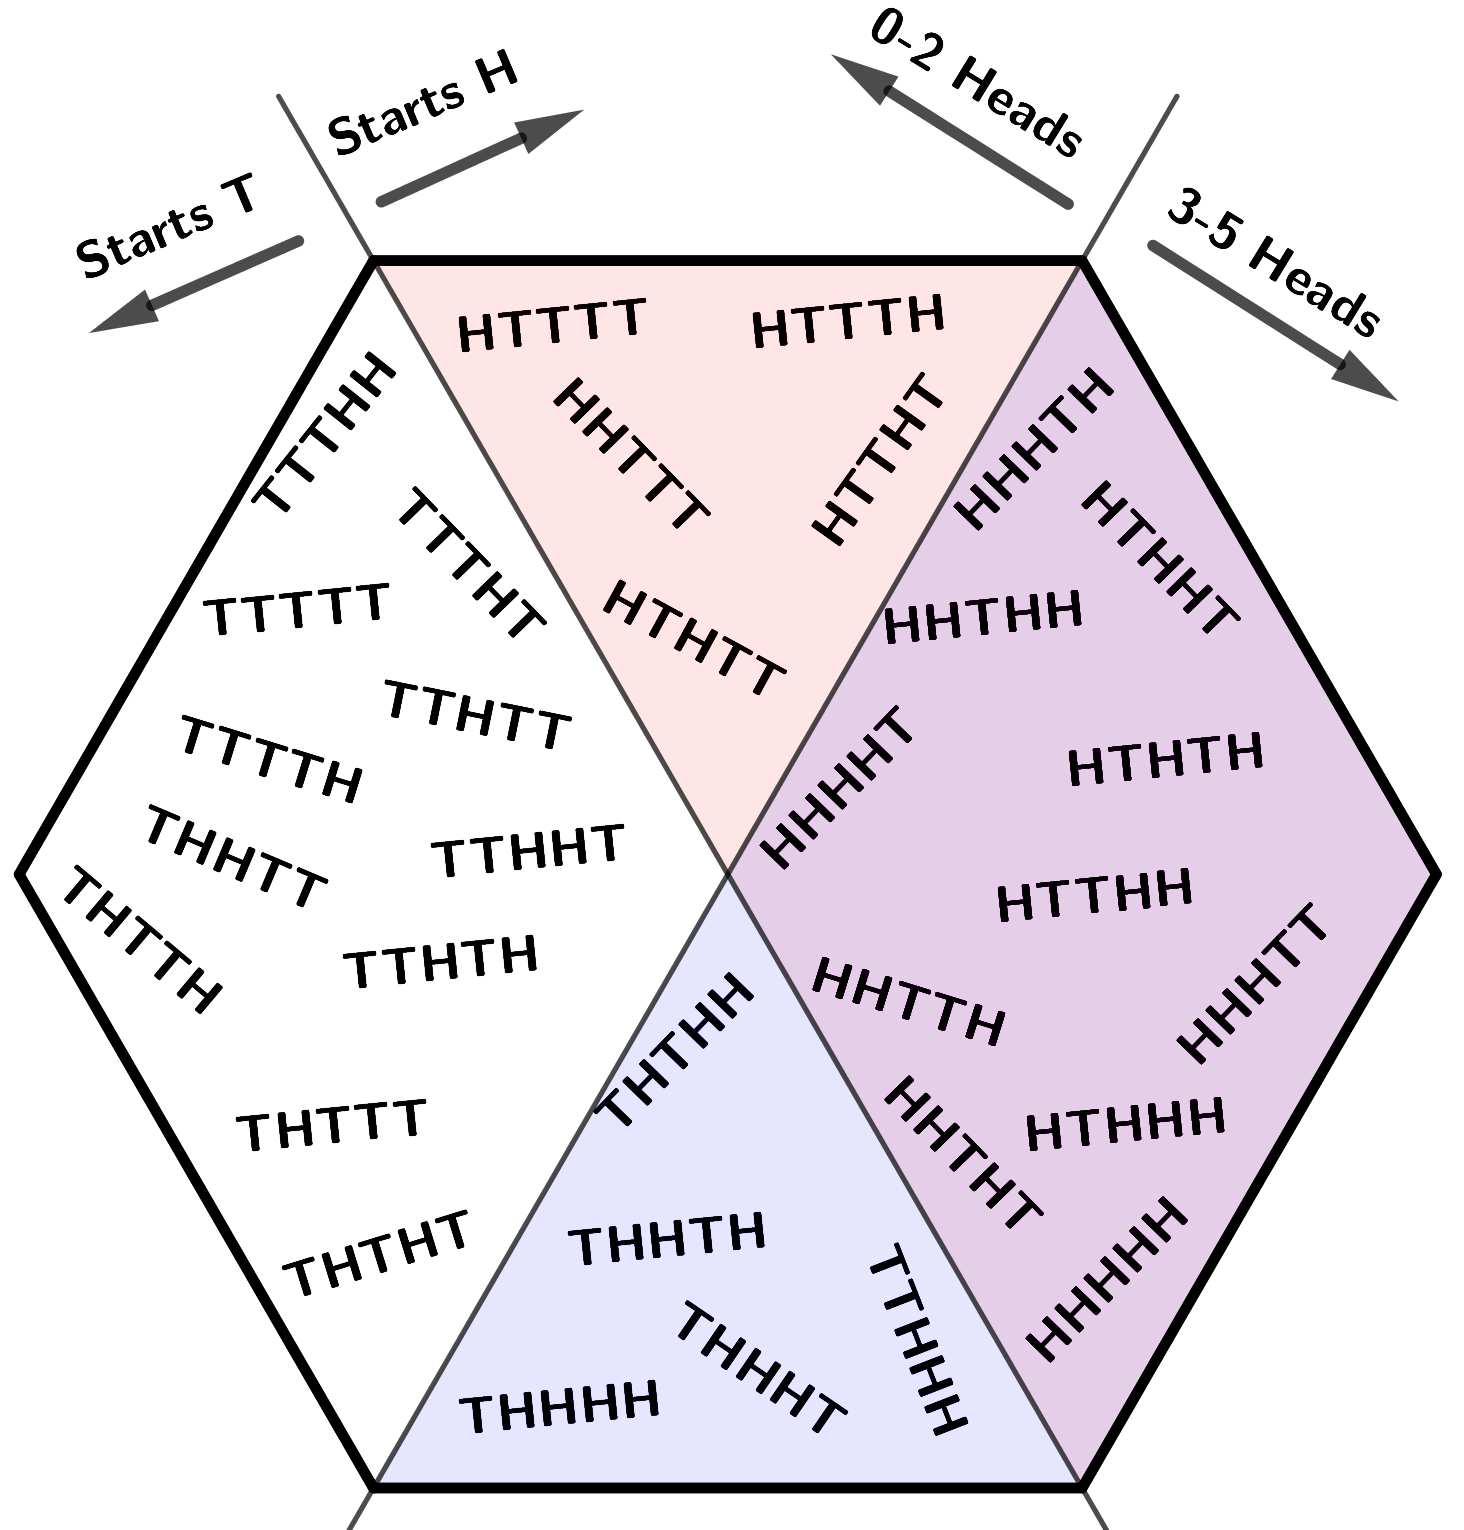
\includegraphics[width=0.52\textwidth]{images/condo0.png}\qquad
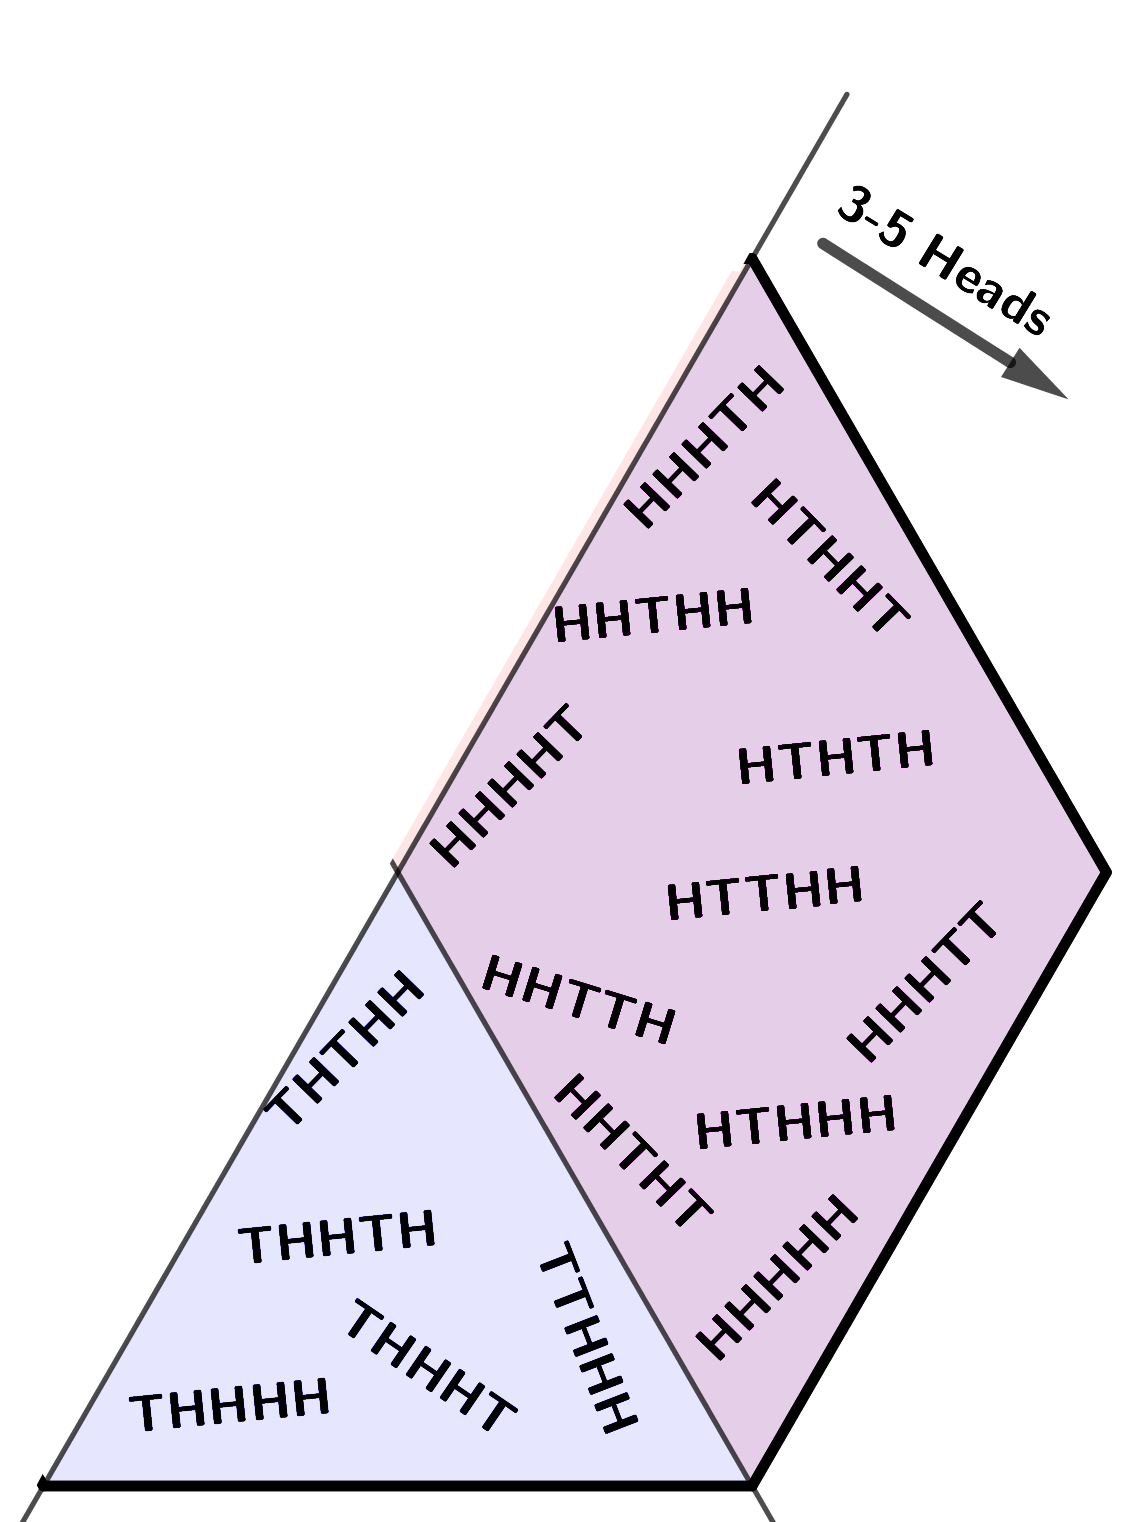
\includegraphics[width=0.4\textwidth]{images/condo1.png}
\caption{\label{condo} The whole sample space for 5 coin tosses (left). ``Zooming in'' on the half with $\geq 3$ heads, we see that $11/16$ start with an `H'. So $\PP(\text{starts with H} \st \text{number of H $\geq 3$ }) = 11/16$.} 
\end{figure}

\ssn{Bayes' Theorem} 
Let $A,B$ be events with $\PP(B)\not= 0$.  Then 
\tcb  
\[
    \PP( A \st B) = \PP( B \st A) \frac{\PP(A)}{\PP(B)}.
 \]
\etcb 
\begin{proof}
We compute $\PP(A \cap B)$ in two different ways: 
 \[ 
 \PP(B \st A) \PP(A) = \PP(A \cap B) = \PP(A \st B) \PP(B). 
 \]
Dividing by $B$ gives the result. 
\end{proof}
We could easily have solved the problem above using Bayes' Theorem; it would be essentially the same calculation. 
\end{n}

\ssn{Bayes' Theorem (``probability of causes'' form) }
Let our sample space $S$ be partitioned into disjoint events $A_k, \, k=1,2,\dots, n$.  Then for $1\leq j \leq n$, 
\tcb
\[
   \PP(A_j \st B)  =   \frac{\PP(B \st A_j)\,\PP(A_j)}{ \sum_{k=1}^n \PP(B \st A_k) \,\PP(A_k)}
 \]
 \etcb 
\begin{proof}
Put $A=A_j$ in the previous version of the theorem and then expand $\PP(B)$ using the law of total probability (\S\ref{totprob}).
\end{proof}
\end{n}

\ssn{Example}
The use of the the ``probability of causes'' form is more straightforward than it might appear from the statement. 

Tom and Dick are both liars: independently for everything they say, they tell the truth with probability $1/3$ and lie with probability $2/3$.  Tom says something.  Dick tells me that Tom is telling the truth.  What is the probability that Tom is telling the truth? 


\tikzset{
  treenode/.style = {shape=rectangle, rounded corners,
                     draw, align=center,
                     top color=white, bottom color=blue!30},
  root/.style     = {treenode, font=\Large, bottom color=red!30},
  env/.style      = {treenode},
  branch/.style = {treenode, bottom color=blue!10},  
  dummy/.style    = {circle,draw}
}
\tikzstyle{level 1}=[level distance=4.0cm, sibling distance=3.5cm]
\tikzstyle{level 2}=[level distance=5.0cm, sibling distance=2.0cm]

\begin{tikzpicture}
[
grow=right,
    edge from parent/.style = {draw, -latex},
    every node/.style       = {font=\normalsize}
  ]
\node[root]{Tom speaks}
child { 
    node[branch]{Tom lied}
    child { 
        node[env]{Dick says ``Tom told truth''}  
        edge from parent node[above]{$\frac23$} 
        }       
    child { 
        node[env]{Dick says ``Tom lied''}                 
        edge from parent node[above]{$\frac{1}{3}$} 
        }       
    edge from parent node[above]{$\frac23$}            
    }
child { 
    node[branch]{Tom told truth}
    child { 
        node[env]{Dick says ``Tom lied''}                
        edge from parent node[above]{$\frac{2}{3}$} 
        }       
    child { 
        node[env]{Dick says ``Tom told truth''}               
        edge from parent node[above]{$\frac{1}{3}$} 
        }       
    edge from parent node[above]{$\frac{1}{3}$}            
    }     ;           
\end{tikzpicture}

Here, we let $A_1$ be ``Tom told truth'' and let $A_2$ be ``Tom lied''.    We let $B$ be the event that ``Dick says Tom told truth''. 
We are asked to calculate $\PP( A_1 \st B)$. So, using Bayes' theorem in the ``probability of causes'' version we have 
 \begin{eqnarray*}
   \PP( A_1 \st B) &=& 
     \frac{\PP(B \st A_1) \, \PP(A_1)}
     {  \PP(B \st A_1) \,\PP(A_1) + \PP(B \st A_2)\,
         \PP(A_2)   } \\
    &=& \frac{ (1/3)(1/3)}{(1/3)(1/3)+(2/3)(2/3)}  = \frac15. 
 \end{eqnarray*}
\end{n}

\ssn{Example}
The example we will now study is presented as an ``updating information'' example where we use the original Bayes' theorem.  You might like to convert it to a ``probability of causes'' wording and draw the probability tree to understand the connection.

A suspect X is believed to be guilty of a given crime with probability $\PP(G)=0.6$ on the basis of existing evidence.  The criminal also left a blood stain at the scene. The suspect X has a blood group common to 20\% of the general population.

A test on the blood stain now tells us that it comes from a person with this blood group. How does that affect the probability that the suspect X is guilty? 


Let $B$ be the event that the blood stain has this particular blood group.  We know the blood test will certainly be positive if X is guilty, so $\PP( B \st G) = 1$.  But we want to know the probability of X's guilt, given the new evidence. In other words, we want to find $\PP( G \st B)$. 


First we calculate (law of total probability again) 
 \begin{eqnarray*}
  \PP(B) &=& \PP(\text{X guilty}) \,\PP(B \st \text{X guilty})   + \PP(\text{X not guilty}) \,  \PP(B \st \text{X not guilty} ) \\
  &=& (0.6) (1) + (0.4) (0.2)  = 0.68
 \end{eqnarray*}
 because if X is not guilty, the blood test will be positive with the probability of its being so in the general population.
 
Then according to Bayes' Theorem
 \[
    \PP( G \st B) =  \frac{\PP( B \st G)}{\PP(B)} \, \PP(G)
    =  \frac{1}{0.68} \, 0.6 = 0.88 
 \]
is an updated probability of X's guilt. 

Bayes' Theorem has been widely used in court cases. See \url{https://www.theguardian.com/law/2011/oct/02/formula-justice-bayes-theorem-miscarriage} for a controversy a few years ago around this. (Colin Aitken, until recently in the School of Mathematics in Edinburgh is quoted.) 
\end{n}

\sse{}
I toss a coin 6 times and get a total of four heads. What is the probability my first roll was heads?  (Ans: $2/3$.) 
\end{e}



\subsection{Exercises} 


\sse 
A very standard example of this sort of ``probability of causes'' analysis is ``false positives'' in medicine. For example, suppose that in the general population, a certain condition is present in 1\% of people.  

There is a test for the condition. The test always returns positive if the subject has the condition.  If the subject does not have the condition, it returns negative 95\% of the time but gives a positive response 5\% of the time.  

A random person takes the test and it returns positive. What is the probability they have the disease? 
\end{e}

\sss 
You may find drawing the tree helps.   In this case, let $C$ denote the event that the random person has the condition.  Let $T$ denote the event of a positive test result.  From the question 
 \[  
    \PP(C) = 0.01, \quad \PP(C^c) = 0.99, \quad \PP(T \st C) = 1, 
    \quad \PP( T \st C^c)=0.05
 \] 
 where the complement $C^c$ is the event of the person not having the condition. Finally, 
 \[
 \PP(T) = \PP(T \st C) \PP(C) + \PP(T \st C^c) \PP(C^c) = 
   1 (0.01) + 0.05 ( 0.99) = 0.0496.
 \]
We are asked for $\PP( C \st T)$ and so by Bayes,
\[
   \PP(C \st T) = \PP(T \st C) \,\frac{\PP(C)}{\PP(T)} 
   = 1 \; \frac{0.01}{0.0496} = 0.2016. 
\]
(One sees here a basic problem with ``screening'' programmes: unless the test is very reliable, they will throw up many more false alarms than real ones.) 
\end{s}



\sse 
This sort of information updating with Bayes' Theorem is also an essential ingredient in machine learning. It goes something like this. 

Suppose an image identifying algorithm is trying to decide what sort of animal is appearing in a picture on the web.  The word ``cat'' appears in nearby text so the algorithm's initial hypothesis is it's a cat with probability $0.8$. The algorithm decides that there is a ball of string in the picture. It is known that this is the case for 50\% of cat pictures but also for 10\% of non-cat pictures.  What is the updated probability that the picture shows a cat? 
\end{e}

\sss
Here $P(C)0.8$, where $C$ is the event of the picture being of a cat. The probability of a ball of string in the picture is 
 \[
   \PP(S) = \PP(S \st C) \PP(C) + \PP(S \st C^c) \PP(C^c) = 
    0.5 * 0.8 + 0.1 * 0.2 = 0.42,  
 \]
(where $C^c$ is the complement of $C$, i.e.\ the even of the picture not being of a cat).   So, by Bayes: 
 \[
   \PP(C \st S) = \frac{\PP(S \st C)}{\PP(S)} \,\PP(C) =
       \frac{0.5}{0.42} 0.8 = 0.95.
 \]
\end{s}

\ssp 
Tom, Dick and Harry each tell the truth independently with probability $1/3$ and lie with probability $2/3$ every time they speak. Tom says something we don't hear; Dick states whether Tom told the truth or not, but we don't hear that either. Harry says that Dick says that Tom told the truth.  What is the probability that Tom told the truth? 
\end{e}

\sss
From a tree, I compute that Harry says that Dick says that Tom told the truth (``HSDSTTT") with probability $13/27$. Also, the conditional probability that Harry says this given that Tom told the truth (``TTT'') is $5/9$. From Bayes (or just analysing the tree),
 \[
   \PP(TTT \st HSDSTTT ) = \PP( HSDSTTT \st TTT) \frac{\PP(TTT)}{\PP(HSDSTTT)} = \frac59 \, \frac{1/3}{13/27} = \frac5{13}. 
 \]
\end{s}




\subsection{Independence}

\ssn{Definition: independence} \hfill
\tcb
Two events $A,B \subseteq S$ are \ul{independent} if
 \[
   \PP(A \cap B) = \PP(A) \PP(B). 
 \]
\etcb

\noindent
The event $A \cap B$ is the intersection of the two events: it occurs precisely when both $A$ and $B$ occur. 

We say two events are ``dependent'' if they are not independent. 

We will say more about independence next week.  Two events being independent means that knowing that one has occurred does not change the probability that the other occurs.  
\end{n}

\ssn{Examples}
\begin{itemize}
    \item Roll a D6 twice. Let $A$ be the event that the first roll is a `6' and let $B$ be the event that the second roll is a `6'. Then $\PP(A) = \PP(B) = 1/6$. Then $A \cap B$ is rolling `double-6' which has probability $1/36$. So $A$ and $B$ are independent.  We were using this independence in our calculations with the probability trees above. 
    \item Roll a D6 twice. Let $A$ be the event that the sum of the rolls is $5$ and let $B$ be the event that at least one `1' appears.     Then $A=\{ (1,4), (4,1),(2,3),(3,2) \} $ and so $\PP(A) = 4/36$.   Counting we find $11$ possible rolls contain at least one `1' and so $\PP(B) = 11/36$.    The event $A \cap B = \{ (1,4), (4,1)$ and so $\PP(A \cap B) = 2/36$. Checking 
     \[
        \frac2{36} \not = \frac{4}{36} \, \frac{11}{36}
     \]
     and so $A$ and $B$ are \emph{not} independent. 
      \begin{itemize}
          \item Looking at this from another angle, if we know that the sum is 5, then there are only four possibilities and two of them contain a `1':  the probability now of there being a `1' present is $1/2$. 
      \end{itemize}
\end{itemize}
It is worth noting at this stage that the very last item above is usually expressed in the form 
 \[
  \text{The \ul{conditional probability} of $B$ given $A$ is equal to $1/2$} 
 \]
which we write with the notation 
\[
   \PP( B \st A) = \frac12 
\]
where the vertical bar is read as ``given''. 
We will take up conditional probability further next week. 
\end{n}


\subsection{Random Variables}

\ssn{Definition: Random variable}
For a binomial distribution problem, the sample space $S$ might be taken to be all the possible $2^n$ length-$n$ sequences of successes and failures. But all we are interested in is the number of successes, which is a function on the sample space taking numerical values.  Thus we make the definition:

\tcb
A \ul{random variable} is a function on the sample space.
\etcb 
We usually use capital letters from late in the alphabet (very often $X$) as the symbol for a random variable. 

In probability we will often de-emphasise or even ignore the sample space and work with the random variable directly. 

These capital $X$ random variable gadgets are a bit like the $x$ that appears for a variable in algebra, except that we imagine it takes various different values probabilistically. 

We will assume for now that our random variables, like our sample spaces, are \ul{discrete}; this means that they take a finite or countably infinite number of possible values $x_1, x_2, \dots$.  
\end{n}

\ssn{Uniform random variable}
The \emph{standard uniform random variable} on $\{1,2, \dots , n\}$ is a random variable $X$ such that 
 \[
   \PP(X=k) = \frac1n \quad \text{for $k \in \NN, \;  k \leq n$}
 \]
Rolling an $n$-sided die (which we usually denote `Dn') is assumed to be such a random variable.

We use the symbol `$\sim$' to indicate that a random variable is distributed according to a standard law. Thus here we will sometimes write 
 \[
     X \sim \mathop{Unif}(1,\dots, n). 
 \]
\end{n} 

\ssn{Bernoulli random variable}
A \emph{Bernoulli random variable} with parameter $p$ (where $0 \leq p \leq 1$) is a random variable such that $\PP(X=1) = p$ and $\PP(X=0) = q$ where $q=1-p$. 

We will write $X \sim \mathop{Bern}(p)$ to indicate that $X$ is distributed as a Bernoulli random variable with parameter $p$. 

So a Bernoulli random variable is a one-off trial that succeeds with probability $p$.  It is the trivial $n=1$ case of a binomial random variable.
\end{n}

\ssn{Binomial random variable}
A Binomial random variable with parameters $n \in \NN$ and $p$ (where $0 \leq p \leq 1$) is a random variable taking values $\{ 0,1, \dots , n \}$ with 
 \[
   \PP(X=k) =   \binom nk p^k q^{n-k} =  \frac{n!}{k! \, (n-k)!} p^k q^{n-k}
 \]
 We will write $X \sim \mathop{Binom}(n,p)$ to indicate that $X$ is distributed as a binomial random variable with parameters $n$ and $p$.
\end{n}
 
 \ssn{Events}
 When working with a random variable $X$, events can be defined in terms of the values taken.  So for instance $X=3$ and $1 \leq X \leq 4$ define events. Thus we can refer to their probabilities $\PP(X=3)$ and $\PP( 1 \geq X \leq 4)$. 
\end{n}
 
 \ssn{Definition: Independence of random variables} 
 If we have two random variables $X,Y$ defined on the same sample space we say that
 \tcb 
 $X$ and $Y$ are \ul{independent} if for all values $x,y$ we have 
 \[
     \PP( \text{$X=x$ and $Y=y$} ) \quad = \quad \PP( X=x) \, \PP(Y=y).
  \]
 \etcb 
\end{n}
 

\subsection{The Binomial Distribution}

\ssn{An important example} 
What is the probability that on rolling three D6 I get exactly one `6'? 

There are exactly three routes through the tree that give this outcome and each has probability 
 \[
      \left( \frac16 \right) \left( \frac56 \right)^2 = \frac{25}{216}.
 \]
Thus the probability is 
 \[
     3 \frac{25}{216} = \frac{25}{72}. 
 \] 
\end{n}

\ssn{A generalisation}
Let us consider a general version of the problem.  Supposing we have a process that each time it is carried out produces independently a ``success'' (S) with probability $p$ or a failure (F) with probability $q=1-p$. In the examples in \S\ref{mp2}, success is finding a faulty component or correctly guessing the answer to a question.  We are assuming that each execution of the process is ``independent'', meaning that its success or failure  each time is not influenced by what might have happened before.  If we now repeat this process $n$ times, what is the probability that we get exactly $k$ successes? 
\end{n}




\ssn{Example} 
Suppose $n=10$ and $k=7$ and $p=1/4$. One particular sequence of successes and failures is $SSFFSSFSSS$. Thinking of a large probability tree, the probability of this exact sequence is 
 \[
    ppqqppqppp = p^k q^{n-k} = p^7 q^3 = \left( \frac14 \right)^7 \, \left( \frac34 \right)^3   = \frac{3^3}{4^{10}}
\]
This probability is the same for all the different sequences with seven successes. 

How many other sequences  are there with precisely seven S's?  That is the same question as asking how many ways are there of choosing seven things from ten.  It is the Binomial coefficient
 \[
       \binom{10}7 = \frac{10!}{7! \,3!} = 120. 
  \]
Adding all these possibilities, the probability of three successes in eight trials is exactly 
  \[
     \binom{10}7 p^k q^{n-k} = 120 \frac{3^3}{4^{10}} \approx 0.0031. 
  \]
\end{n}

\sse{}
Note that we have just derived the probability of getting exactly 7 out of 10 by guessing in our multiple choice quiz. Work out the probability of getting 8, 9 and 10 out of 10 and hence answer our second motivating problem. 
\end{e}

\sss
\[
    \binom{10}{7} \left( \frac13\right)^7 \left( \frac23 \right)^3 +  
    \binom{10}{8} \left( \frac13\right)^8 \left( \frac23 \right)^2 +  
    \binom{10}{9} \left( \frac13\right)^9 \left( \frac23 \right)^1 +  
    \binom{10}{10} \left( \frac13\right)^{10} \left( \frac23 \right)^0  \approx 0.019661636.
 \]
 (I give many decimal places because leaving out the 1/10 possibility only affects the fifth decimal place!) 
\end{s}


\ssn{} 
For the general problem, the probability of $k$ successes in $n$ trials is as follows.  
\tcb 
\ul{Binomial distribution} 
  \[
       \PP( \text{$k$ successes}) =  \binom nk p^k q^{n-k} =  \frac{n!}{k! \, (n-k)!} p^k q^{n-k}. 
  \]
 \etcb 
\end{n}

\ssn{Example}
I roll a D6 twelve times.  How likely is it that I roll precisely two sixes?   Here, $n=12, k=2$ and $p=1/6$. So the answer is 
 \[
    \binom{12}2 \left(\frac{1}{6}\right)^2  \left(\frac{5}{6}\right)^{10}
     \approx 0.296.
 \]
\end{n}

\sse{Exercise}
I toss a fair coin 6 times.  How likely is it that I roll $k$ heads where $k=0,1,2,3,4,5,6$? 
\end{e}
\sss 
Use the formula with $n=6$ and $p=1/2$.  For instance, $\PP(k=3) = 20/64 = 5/16$. 
\end{s}



\begin{table}[h]  
  \begin{tabular}{cc} 
    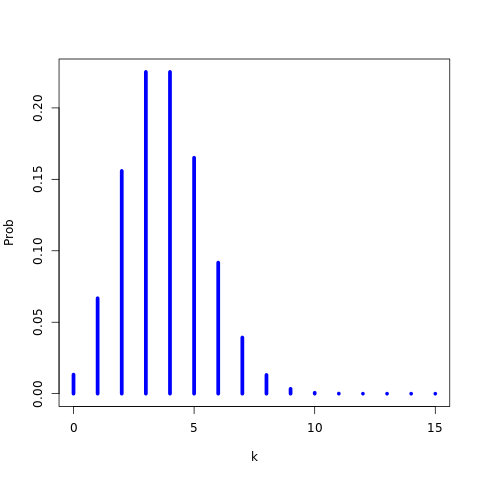
\includegraphics[width=0.45\textwidth]{images/binom15P25.png} & 
    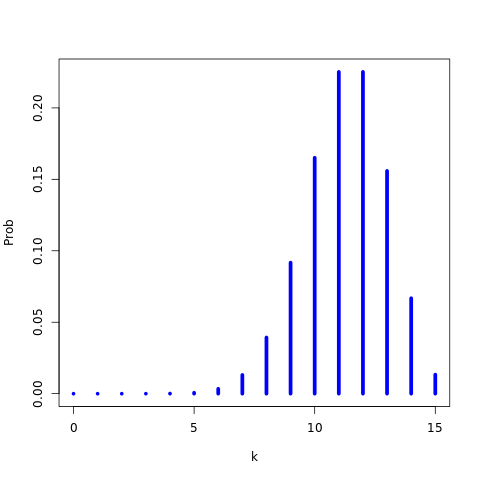
\includegraphics[width=0.45\textwidth]{images/binom15P75.png} \\
     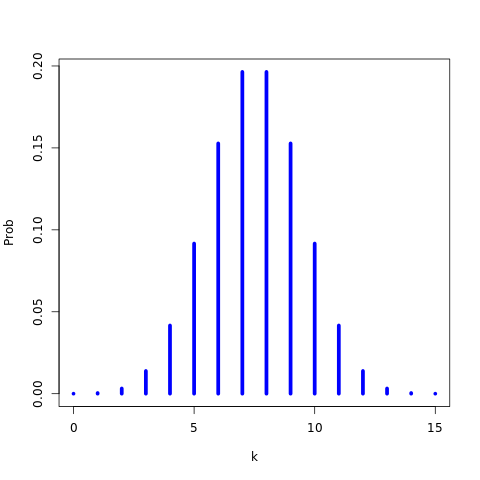
\includegraphics[width=0.45\textwidth]{images/binom15P5.png} & 
    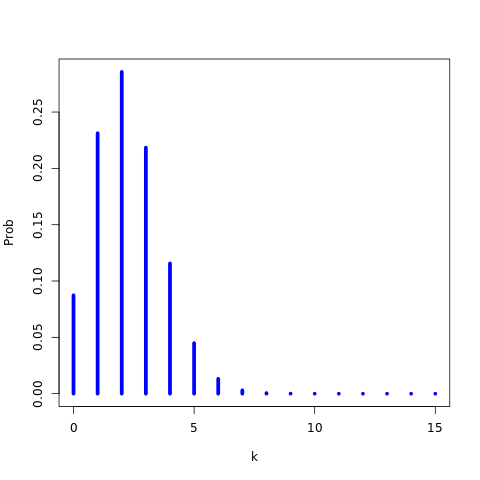
\includegraphics[width=0.45\textwidth]{images/binom15P15.png} \\
  \end{tabular}
 \caption{\label{binpics} Binomial with $n=15$ and $p=0.15, 0.25, 0.5, 0.75$ in some order}
\end{table}


\sse
In table~\ref{binpics} ``probability mass functions'' for Binomial distributions with different probabilities are plotted. The height of each vertical bar is the probability of the corresponding outcome. Which is which?
\end{e}

\sss
The top row has $p=0.25$ and $p=0.75$. Note the symmetry between them. 
The bottom two are $p=0.5$ (note the symmetry about its centre) and $p=0.15$. 
\end{s}

\sse{}
\begin{enumerate}
    \item 
Compute the `Red v Blue' and `Green v Red' probabilities with a tree.
 \item Compute the win probability of Blue versus Green where the game is to roll two blue dice versus two green dice with the higher total winning. 
\end{enumerate}
Answers to these can be found in the Workshop 1 solutions. 
\end{e}



%%Week 03
\section{More discrete and continuous distributions}
%\ssn{Learning Outcomes}
%After studying this week you will be able to:
%\begin{itemize}
%\item use the geometric distribution to calculate probabilities;
%\item explain what is meant by a continuous random variable and how it is represented by a probability density function;
%\item compute probabilities and expectations for continuous random variables;
%\item model appropriate problems using exponential or uniform distributions.
%\end{itemize}
%\end{n}

\subsection{Geometric Distribution}

\ssn{Motivating problem} 
I have a process which, independently I execute it, has a probability $p$ of success. Let $X$ be the number of tries up to and including my first success. What is the probability that $\PP(X=k)$, i.e.\ I succeed for the first time on my $k$-th try. 

Setting $q=1-p$, to succeed on the $k$-th attempt, I have to fail $k-1$ times in a row and then succeed. Since the tries are all independent, we have 
 \[
         \PP(X=k) = q^{k-1} p. 
  \] 
\end{n}

\ssn{Definition: Geometric random variable} 
A random variable $X$ is \ul{geometric} and we write $X \sim \mathop{Geom}(p)$ if \hfill 
 \tcb 
   \[
         \PP(X=k) = q^{k-1} p \quad \text{where $q=1-p$.} 
  \] 
 \etcb
\end{n} 

\ssn{Proposition}  The expected value of $X \sim  \mathop{Geom}(p)$ is $\EE(X) = 1/p$. 
\begin{proof}
From the definition of $\EE(X)$ we have 
 \[
     \EE(X) = p + 2pq + 3pq^2 + 4 pq^3 + \dots .
 \]
Multiplying by $q$ we have 
 \[
      q \EE(X) = pq + 2pq^2 + 3pq^3 +  \dots .
 \]
 Subtracting
  \[
  (1-q) \EE(X) = p \EE(X) =  p + pq + pq^2 + pq^3 + \dots = \frac{p}{1-q} = 1.
  \]
 where we have summed the GP and used $q=1-p$. 
\end{proof}
\end{n}

\ssn{Example} 
 Suppose I roll a pair of D6 repeatedly I and count the number of rolls until I roll a total of `5'.  The probability of rolling a total of five is $4/36 = 1/9$. 
 
 So with $X \sim \mathop{Geom}(1/9)$ we have that the probability of succeeding first on the third roll is 
  \[
       \PP(X = 3) = q^2 p = \left( \frac89 \right)^2   \frac19 = 
       \frac{64}{729}.
  \]
  The expected number of rolls is $\EE(X) = 1/p = 9$. 
\end{n} 

\sse{Exercise} 
One day each week I go fishing in a lake and  I independently have a probability of $1/52$ of catching the big carp that lives there.
Let $X=k$ if I first catch the carp on my $k$-th day fishing. 
\begin{enumerate}
    \item On which day of fishing am I most likely to catch the carp? 
    \item What is the probability that I first catch the carp on my third day fishing? 
    \item What is the expected number of fishing days until I catch the carp? 
\end{enumerate}
\end{e}

\sss
Here $X \sim \mathop{Geom}(1/52)$. The value of $\PP(X=k)$ is greatest when $k=1$ and so the first day is the most probable day that I catch the fish.  The probability of first catching it on day 3 is $(51/52)^2 (1/52)$.  The expected number of days is $1/p$ = $52$. 
\end{s} 


\subsection{Continuous distributions}

\ssn{Exponential distribution: Motivating problem}
Radioactive atoms spontaneously decay after a certain time by emitting a particle.  It works like this. If the atom has not yet decayed at a given moment, then the probability of its decaying in the next short time $\Delta t$ is (in the limit as $\Delta t \map 0$) equal to $\lambda \Delta t$ where $\lambda$ is a constant for the particular type of atom. It does not matter if the atom in question has been around for millennia or if it was created a second ago, the chances of its decaying in the next second are the same.  So if we say we have an intact atom now at time $t=0$ what can we say about the probability of its decaying within a certain time?  
\end{n}

\ssn{The problem} 
We have a random variable $T$ here with sample space $[0,\infty)$, with the point $t$ corresponding to decay at time exactly $t$.  What is the probability of decay at time exactly $t=7.5$?  
Letting $T$ denote the random variable that is the time of decay, 
The answer is that $\PP(T=7.5) = 0$.  This is
because if the probability was equal to some positive number $\epsilon >0$ then you could find uncountably many very nearby values of $t$ which would have to have about the same probability, and then these probabilities would add up to more than $1$. So we proceed as below. 
\end{n}

\ssn{Probability density functions} \hfill 
\tcb 
A \ul{probability density function} (\emph{pdf} for short) for a random variable $X$ on a (possibly infinite) interval $I$ is a piecewise continuous function $f_X:I \map \RR$ satisfying 
\begin{enumerate}
\item $f_X(x) \geq 0$ for all $x \in I$; 
\item $\int_I f_X(x) \dd x = 1$. 
\end{enumerate}
\etcb 
\noindent The interpretation of $f_X$ is that for $a,b \in I$ with $a \leq b$ we have   
\tbc
\[
    \PP ( a \leq X \leq b ) = \int_a^b f_X(x) \dd x. 
\]
\etbc 
We will sometimes think of $f_X$ as being defined on all of $\RR$ but equal to zero outside of our interval $I$. 
\end{n}

\ssn{Example} 
A thin rod of length $L$ breaks at a single point equally likely to be anywhere along the rod. Let the random variable that is the break point be $X$. The sample space can be taken to be $[0,L]$. Since the break is equally likely to be anywhere, the pdf will be constant. For it to have integral $1$ on $[0,L]$ we must have $f_X(x) = 1/L$. 

What is the probability that the break is in the centre third of the rod? Common sense tells us immediately that it should be $1/3$.  Checking with the integral we see that 
 \[
    \PP( L/3 \leq X \leq 2L/3 ) = \int_{L/3}^{2L/3}  \frac{1}{L} \dd x = 
      \left[  \frac{x}{L} \right]_{L/3}^{2L/3} = \frac{1}{3}. 
 \]
\end{n}

\ssn{Definition: Uniform distribution} A continuous random variable $X$ is said to be \ul{uniform} and we write $X \sim \mathop{Unif}(a,b)$ if $X$ has a constant pdf 
 \[
      f_X(x) = \frac1{b-a}  \quad \text{for $a \leq x \leq b$}. 
 \]
\end{n} 

\sse 
\begin{enumerate}[(a)] 
\item For what value of the constant $a$ does $f_X(x)=ax$ define a pdf on $[0,1]$?
\item For what values of $x$ is $f_X(x)>1$? (NOTE: The point of this part is to draw attention to the fact that $f_X(x)$ is NOT a probability and can be greater than $1$.)  
\end{enumerate}
\end{e}

\sss 
Integrating or drawing a picture, $k=2$ is required.   So $f_X(x)>1$ in the right-hand half of the interval.
\end{s}


\ssn{Definition} \hfill 
 \tcb 
  Let $f_X$ be a pdf for a random variable.  The \emph{cumulative distribution function (cdf)} is defined by  
  \[
    F_X( x) = \PP( X \leq x ) = \int_{-\infty}^x  f_X(u) \dd u.  
   \]
 \etcb 
 \noindent 
 We often abbreviate by missing one of the three words from ``cumulative distribution function''. The cdf make sense also for discrete variables, but appears more in continuous problems. 
\end{n}

\ssn{Proposition} \hfill 
\label{PropCdfPdf}
 \tcb 
\begin{itemize}
\item Away from points where $f_X$ is not continuous, $F_X$ is differentiable and $F_X'(x) = f_X(x)$.
\item The cdf $F_X(x)$ is non-decreasing.
 \item If $X$ takes values only in an interval $[a,b]$, so that $f_X(x) = 0$ outside that range, we have $F_X(x)=0$ for $x \leq a$ and $F_X(x)=1$ for $x \geq b$. 
\end{itemize}
 \etcb 
\begin{proof}
The first property is the Fundamental theorem of Calculus.  The second and third come from the definition of $F$. 
\end{proof}
\end{n}

\ssn{Examples}
\begin{itemize}
\item For the rod example $f_X(x) = 1/L$ for $0 \leq x \leq L$ and $f_X = 0$ otherwise. The cdf is 
 \[
        F_X(x) = \int_{-\infty}^x f_X(u)  \dd u = \begin{cases} 0 & \text{for $x < 0$} \\
        x/L  & \text{for $0 \leq x \leq L$} \\
        1 & \text{for $x >  L$}  \end{cases} 
 \]
 The interpretation of $F_X(x)$ is that it is the probability of the break occurring to the left of $x$. 
 \item For the exponential distribution if $f_X(x) = \lambda e^{-\lambda x}$ for $ x \geq 0$ and zero otherwise. So $F_X(x) = 0$ for $x \leq 0$ and otherwise 
  \[
    F_X(x) =   \int_0^x \lambda e^{-\lambda u} \dd u = \left[  e^{-\lambda u}   \right]_0^x = 1-  e^{-\lambda x} . 
  \]
 It is the probability of the atom decaying  before time $t$. The picture shows the pdf and cdf for this distribution with $\lambda=1.5$. 
 \begin{center}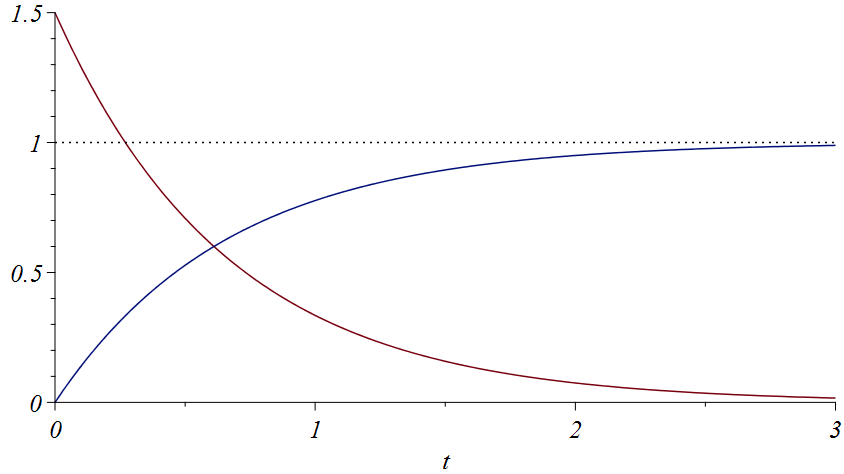
\includegraphics[width=0.7\textwidth]{images/exp-cum.png}
  \end{center}
\end{itemize}
\end{n}


\ssn{Foundations}
We will not present a completely rigorous version of the foundations of continuous probability. The fundamental difficulty is that an event will be a subset of the sample space and it needs to be a subset over which a suitable pdf can be integrated, and we do not study integration rigorously until later in the degree.  We will only consider events that are finite unions of intervals. 

Given that we assume that $f_X(x)$ is piecewise continuous,  $\int_x^x f_X(u) \dd u = 0$ and we are forced to have $\PP(X=x) = 0$ for all points $a$.   Consequently it does not matter if endpoints are included because $\PP(X<x) = \PP(X \leq x)$ and so on. 

We will assume that probabilities for events obey the fundamental properties in \S\ref{prprops} without proof.    
\end{n}


\subsection{Exponential Distribution}

\ssn{Example: back to the radioactive atom} (Do not get bogged down in the following argument if you find parts of it hard. The main point is that at the end we derive a pdf for the situation. The derivation is not examinable.)  

Let us return to the radioactive atom and see if we can find a candidate for a pdf. We will assume there is a constant $\lambda >0$ such that \emph{if the atom is intact at time $t$} then it decays in the interval $[t, t + \Delta t]$ with probability $\lambda \Delta t$ (in the limit as $\Delta t \map 0$).

Now, letting $T$ be the RV which is when the atom decays and letting its pdf be $f_T$ we have the following as $\Delta t\map 0$.
\begin{eqnarray*}
  f_T(t) \Delta t &=& \PP (t \leq T \leq t+\Delta t) \\
   &=& \PP(\text{intact at time $t$}) \;\PP( \text{decays in $[t,t+\Delta t] \st$ intact at time $t$})  \\
   &=& \PP(\text{intact at time $t$}) \lambda \Delta t  \\
   &=& (1- \PP( 0 \leq T \leq t))  \lambda \Delta t.  
\end{eqnarray*}
Dividing be $\Delta t$ and replacing the probability by an integral of the pdf we have
\[
   f_T(t) = \lambda \left( 1 - \int_0^t f_T(u) \dd u \right). 
\]
Differentiating, we have 
 \[
   f_T'(t) = -\lambda f_T(t) \text{ and so } f_T(t) = A e^{-\lambda t} \text{ for some $A>0$}.  
 \]
For $\int_0^\infty f_T(t) \dd t = 1$ we need $A=\lambda$ and so finally we have 
\[
     f_T(t) = \lambda e^{-\lambda t} ,\quad t \geq 0. 
\]
\end{n}

\ssn{Definition} \hfill 
\tcb 
A random variable $X$ on $[0,\infty]$ with pdf of the form 
 \[ 
 f_X(x) = \lambda e^{-\lambda x} \text{ (where } \lambda >0
  \]
  is a constant) is called an \emph{exponential random variable}.  
\etcb 
So the sample space is $S = [a,b]$. It does not matter whether we take an open interval $(a,b)$ instead.  
\end{n}

\sse 
\begin{enumerate}[(a)]
\item Show that the probability of decay occurring between the times $t=0$ and $t=1/\lambda$ is $(e-1)/e \approx 0.632$.
\item The \emph{half life} $\tau$ of a radioactive atom is the time at which there is a 50\% chance that an atom that was intact at $t=0$ will have decayed.   Show that $\tau = \ln 2 / \lambda$. 
\end{enumerate}
\end{e}

\sss
\begin{enumerate}[(a)]
\item  We compute 
  \[
     \int_0^{1/\lambda} \lambda e^{-\lambda t} \dd t = [ 1 - e^{-\lambda t}]_0^{1/\lambda} = \frac{e-1}{e}. 
  \]
 \item To find $\tau$ such that the probability of decay is $1/2$ we solve   
 \[
   [ 1-e^{-\lambda}]_0^\tau = \frac12  
 \]
to get $e^{-\lambda\tau}= 1/2$ or $\lambda\tau = \ln 2$. 
\end{enumerate}
\end{s}



\sse{} In a model of a call centre, at a given moment, the time in seconds until the next call arrives is a random variable $T$ that has a pdf of the form 
 \[
    f_T(t) =  k e^{-t/8}, \qquad \text{where $t \in [0,\infty)$ and $k$ is a constant to be determined.}
 \] 
What is the probability that a call arrives in the first four seconds?   (Answers: $k=1/8$ comparing with the general exponential distribution. The integral for the probability should evaluate to approx 0.3935.) 
 \end{e}

\sse{}
The random variable $X$ defined on the interval $[0,1]$ has pdf given by $f_X(x) = k \sqrt{1-x^2}$.  Find the value for $k$. No explicit integration should be necessary! 
(You should arrive at $k=4/\pi$.) 
\end{e}

\sss
Notice that the graph of $y = \sqrt{1-x^2}$ is a quarter of a unit circle so the area under it is $\pi/4$.  Alternatively, integrate!
\end{s}


\ssn{Convention} 
Henceforth we will assume that for a continuous random variables $X$, the pdf $f_X(x)$ is defined for the whole real line. If $X$ takes values only in an interval $(a,b)$ we simply take $f_X(x) =0$ for all $x$ outside $(a,b)$. 
\end{n}


\subsection{Poisson Distribution}

\ssn{Motivating problem}
\begin{itemize}
\item During busy times, calls arrive at a call centre at an average rate of 10 per minute.  What is the probability of four or more arriving in a period of twelve seconds?
\item Huge numbers of dust particles drift around in a large volume. On average, there are $10^6$ per cubic metre. How probable is it that at a certain moment, a cubic centimetre contains three or more particles. 
\end{itemize}
\end{n}

\ssn{A possible model}
For the call centre, if one expects 10 calls per minute, then one expects 2 calls in 12 seconds. One might imagine that those 2 calls arise because there are $n=1000$ customers, each independently with a probability $p=0.002$ of calling during that minute. Or possibly one has $n=10000$ and $p=0.0002$.   With either assumption, we could calculate probabilities with a binomial random variable. 

The problem is that we do not know the values of $n$ and $p$; we know only that the expected number of calls is $np=2$.  In this sort of situation, we really do not want an unknown large $n$ hanging around. Instead we take a limit as $n \map \infty$ keeping $np$ constant. 
\end{n}

\ssn{Taking the limit}
Suppose we fix $\lambda>0$ (where $\lambda=2$ in the example above). Set $p=\lambda/n$ so that the expected value of a binomial $(n,p)$ random variable $X$ is $np=\lambda$. Then 
 \begin{eqnarray*}
 \PP(X=k) &=& \binom{n}{k} p^k (1-p)^{n-k} = \binom{n}{k} 
      \left( \frac{\lambda}n \right)^k 
       \left( 1-\frac{\lambda}n \right)^{n-k}  \\ 
   &=& \frac{n!}{k! (n-k)!} \frac{\lambda^k}{n^k} 
      \left( 1-\frac{\lambda}n \right)^{-k} \left( 1-\frac{\lambda}n \right)^{n}  \\
      &=& \frac{\lambda^k}{k!} \; \underbrace{\frac{n(n-1)\dots(n-k+1)}{n^k}}_{\text{Limit = 1}} \;\;
      \underbrace{\left( 1-\frac{\lambda}n \right)^{-k}}_{\text{Limit = 1}} \;\;    
      \underbrace{ \left( 1-\frac{\lambda}n \right)^{n}}_{\text{Limit = $e^{-\lambda}$}}\\ 
   &\map& e^{-\lambda} \frac{\lambda^k}{k!} \qquad \text{as $n$ tends to infinity.}
 \end{eqnarray*}
 Of the three limits, the first can be seen by dividing top and bottom by $n^k$; the second is because $(1-\lambda/n) \map 1$ as $n\map\infty$ and $k$ is a fixed number; the last is a standard result. 
\end{n}

\ssn{Definition: Poisson distribution} \hfill 
\tcb 
A random variable $X$ on $\{0,1,2,\dots\}$ such that 
 \[
      \PP(X=k) = e^{-\lambda} \frac{\lambda^k}{k!}
  \]
is called a \emph{Poisson random variable with parameter $\lambda$}. 
\etcb 

\noindent 
We should check that this really does define a random variable, i.e.\ that the sum of all the probabilities is equal to one.  That is the case since 
\[
 \sum_0^\infty \PP(X=k) = e^{-\lambda} \sum_0^\infty \frac{\lambda^k}{k!} = e^{-\lambda}  e^\lambda = 1. 
\]
\end{n}

\ssn{Mean and variance}
Let's calculate the probability generating function of a Poisson RV with parameter $\lambda$.  
\[
  G_X(s) = \EE(s^X) = \sum_{k=0}^\infty e^{-\lambda} \frac{\lambda^k}{k!} s^k = e^{-\lambda} e^{\lambda s} = e^{\lambda(s-1)}. 
\]
Then $G_X'(s) = \lambda e^{\lambda(s-1)}$ and $G_X''(s) = \lambda^2 e^{\lambda(s-1)}$.   So 
 \[
  \EE(X) = G_X'(1) = \lambda, \qquad \var(X) = G_X''(1) + G_X'(1) 
    - \left( G_X'(1) \right)^2 = \lambda. 
 \]
\end{n}

\ssn{Example} 
For the call centre example above, the expected number of calls in 12 seconds is one fifth the number expected in a minute.  So $\lambda = 2$. 
So, from the formula, 
 \begin{gather*} 
  \PP(X=0) = e^{-2} \approx 0.135335, \quad \PP(X=1) = 2 e^{-2} \approx 0.270671 ,  \\ 
   \PP(X=2) = 2 e^{-2} \approx 0.270671 , \quad 
   \PP(X=3) = \frac43 e^{-2} \approx 0.180447
 \end{gather*} 
Then adding these and subtracting from one we get $\PP(X\geq 4) \approx 0.142876$. 
\end{n}


\ssn{Example} 
We could also use the Poisson distribution to approximate the Binomial distribution where $n$ is large and $p$ small.  For example, we could ask what the probability is of 5 treble-6 in 1000 tosses of three D6. The exact binomial answer is 
 \[
    \PP (X=5) = \binom{1000}{5} \left(\frac{215}{216}\right)^{995} \left(\frac1{216} \right)^5 \approx 0.17337.
 \]
The expected value here is ``$np$'' is $1000/216$ and number of occurrences is $5$.  So the Poisson approximation gives 
 \[
    e^{-1000/216}  \left(\frac{1000}{216} \right)^5 \frac 1{5!} \approx 0.17295.
 \]
\end{n}

\sse{}
Assume that dust particles drift around at random within some large volume.  The density of dust particles is $10^7$ per cubic metre.  I take a sample of 1cc volume.  What is the probability of their being $k$ dust particles in my sample? 
\end{e}

\sss
To start, $1cc$ is $10^{-6}$ cubic metres.  So the expected number of particles is $\lambda=10$.  Thus from Poisson:
\[
    \PP(X=k) = e^{-10} \frac{10^k}{k!}.
\]
So, for instance, the probability of exactly 10 particles is about 0.125 and the probability of none at all is about 0.0000454. 
\end{s}

\sse 
Studies in the 1990s concluded that computer memory suffered corruption because of a cosmic ray at a rate of one incident per 256Mb per month. On that basis, what is the approximate probability 2Gb of memory being corrupted by a cosmic ray twice in a day?  (Make the possibly unrealistic assumption that the probability is proportional to memory size.) 
\end{e}

\sss 
  Assuming 30 days per month, the expected number per day is $8/30$. We compute 1 minus the probability of zero and one strikes:
  \[
    1 - e^{-8/30} - e^{-8/30} \frac{8}{30} \approx 0.03. 
  \]
\end{s}

\sse 
In a situation where occurrences are modelled by a Poisson random variable, what is the expected time until the next occurrence? 
\end{e}

\sss 
Time to next occurrence is exponential with parameter $\lambda$ and so the expected time is $1/\lambda$. 
\end{s}

\sse 
Buses arrive at a bus stop randomly at an average rate of one every five minutes. I arrive at the bus stop. Assuming a Poisson distribution, find the probability that in the first 10 minutes no bus arrives, and then three arrive at once.   (Interpret ``three arrive at once'' to mean that in the next minute exactly three arrive.) 
\end{e}

\sss 
$0.0001477$. 
\end{s}



\ssn{Proposition}
Let $X_1$ and $X_2$ be independent Poisson random variables with parameters $\lambda_1, \lambda_2$ respectively. Then $X = X_1 + X_2$ is a Poisson random variable with parameter$\lambda = \lambda_1 + \lambda_2$. 

\begin{proof}
The pgfs for $X_1,X_2$ are $G_{X_1}(s)=e^{\lambda_1(s-1)}$ and $G_{X_2}(s)=e^{\lambda_2(s-1)}$. The pgf for the sum of independent RVs is the product of the generating functions and so the pgf of $X$ is $G_{X_1}(s)=e^{(\lambda_1+\lambda_2)(s-1)}$ which we recognise as the pgf of a Poisson RV\footnote{In the argument we are using the fact that the pgf determines the distribution. This is clear in the case of discrete RVs taking finitely many values but really needs further justification generally.} with parameter $\lambda_1 + \lambda_2$. 
\end{proof}
\end{n}

\ssn{Comment}
The property in the theorem is essential in the situations we are modelling. Suppose that $X_1$ and $X_2$ are Poisson RVs modelling the number of calls arriving at a call centre in two consecutive minutes. Then $X_1+X_2$ needs to model the number of calls arriving in the complete two minute period.  
\end{n}

\ssn{Relation with exponential distribution}
Consider a process like the arrival of calls at a call centre which we are modelling using a Poisson random variable assuming an average rate of $\mu$ per unit time. 

Starting at time $t=0$, the next call will arrive at some time $T$ which itself is a continuous random variable on $[0,\infty)$.   We can compute the pdf of $T$.   At time $t$ the expected number of calls to have occurred since $t=0$ is $\lambda = \mu t$. Thus we can use the Poisson distribution to compute 
 \[
   \PP( \text{No calls in [0,t]}) = e^{-\lambda} = e^{-\mu t}.
 \]
So the cdf of $T$ (i.e. the probability of a call having arrived during $[0,t)$ is $F_T(t) = 1 - e^{-\mu t}$ so 
 \[
 f_T(t) = F_T'(t) = \mu e^{-\mu t}.
  \]
 So from any base time, ``time to next occurrence'' is an exponential RV with parameter $\mu$. 
\end{n}



\subsection{Exercises and problems}

\sse 
Invent a random variable $X$ that is sufficiently simple that you can compute its expected value $\EE(X)$, the value of $\EE(x^2)$ and its cdf $F_X(x)$.   
\end{e}

\sse{}
Let $X \sim \gamm(z,\lambda)$.  Compute $\EE(X^2)$.   (Ans: $z(z+1)/\lambda^2$) 
\end{e}

\sse{}
Let $X \sim \geom(\lambda)$.  Compute $\EE(X^2)$.   (Ans: $2/\lambda^2$) 
\end{e}

\ssp{}
A room has two new light bulbs fitted and left permanently on at time $t=0$. They are the only illumination in the room. Each one independently has a failure time described by an exponential random variable $T$ with parameter $\lambda = 1$. 
\begin{enumerate}
    \item Write down the pdf, cdf and expected value of $T$.
    \item Consider a time $t=x$. What is the probability that both bulbs have failed (and so the room is dark) at the time $t=x$? 
    \item Let $X$ be the random variable which is the time that the room goes dark.  Compute the pdf of $X$ and its expected value. 
\end{enumerate}
(Hint: the second part is asking you to calculate the cdf of $X$.) 
\end{e}



\sse 
Evaluate
\begin{enumerate}
\item Let $X$ be the result of rolling a D6. What is the probability of $X=6$ given that $X$ is even?  What is the expected value of $X$ given that $X$ is even? 
\item Rolling a D6, let $Y$ be the number of rolls it takes until I roll a `6'. What is the probability that $Y=5$ given that $Y>3$? 
\item Rolling a D6 again, what is the expected total number of `6's I roll in 8 attempts, given that my first two rolls are 6,2?  
\end{enumerate}
Answers: (1) $1/3$, $4$; (2) $5/36$; (3) $2$.  
\end{e}

\ssp{} This (optional) problem solves the question about ``stopping at the largest number'' from the first lecture in the limit as $n\map \infty$.  We will play fast and loose with limits, and so this derivation is not entirely rigorous. The problem is equivalent to the following. 

Consider numbers $x_0,x_1,x_2,\dots,x_{n-1}$ where the numbers are in \emph{decreasing} order.  Now arrange the $n$ numbers in a list in a random order.  Choose a number $0 < \alpha < 1 $.  Consider the ``initial segment'' consisting of the first $\alpha N$ numbers in the list (of course, $\alpha n$ is not necessarily an integer, but choose the integer that's closest). 

Let the RV $K$ be defined by $K=k$ if $x_k$ is the largest number in the initial segment.    Now find the first number in the list that is larger than $x_K$: what is the probability $\PP(W)$ where $W$ is the event that this is $x_0$, the largest of all the numbers?  

We will answer this in the limit as $n \map \infty$. We calculate $p$ by conditioning on the value of $k$ where $k$ is the smallest value such that $x_k$ is in the initial segment. 
\begin{enumerate}
    \item Explain why $\PP(W \st k=0) = 0$.
    \item Explain why in the limit $n \map \infty$ we have $\PP(K=k) = \alpha (1-\alpha)^k$ for $k < n-k$. 
    \item Explain why $\PP(W \st K=k) = \frac1k$ for $k \geq 1$.
    \item Justify (as far as you can) the claim that  as $n \map \infty$ we have 
     \[
        \PP(W) \approx \alpha \sum_{k=1}^\infty (1-\alpha)^k \frac1k.  
     \]
     \item Comparing with the Taylor series for $\log(1-x)$, deduce that \[
           \PP(W) \approx - \alpha \log(\alpha).
     \]
     \item Use calculus to deduce that $\PP(W)$ is maximised by taking $\alpha = 1/e$ and the maximum value is also $1/e$. 
\end{enumerate}
\end{e}


%%Week 04
\section{Expectation}

\subsection{Idea and definition}

\ssn{The idea of expected value}
Roll a 4-sided die 1000 times and add together your scores. You would expect to roll about 250 each of 1,2,3 and 4 and if you did that exactly you would score 
\[
   (250 \times 1) +  (250 \times 2) + (250 \times 3) + (250 \times 4 ) = 2500.  
\]
You could rewrite that as 
\[
  1000 \left( \left( \frac{1}{4}  \times 1\right) 
   + \left( \frac{1}{4}  \times 2\right) 
   +\left( \frac{1}{4}  \times 3\right) +\left( \frac{1}{4}  \times 4\right) \right) = 1000 \times \frac{5}{2}    
\]
and we see that each roll of the die contributes an ``expected value'' of $\frac{5}{2}$ to the total. 
\end{n}

\ssn{Definition: Expected value}
Suppose that the random variable $X$ takes a finite or countable number of different numerical values $x_i$. Let the probability that $X$ takes the value $x_i$ be denoted $p_i$ so that 
 \[
     \PP (X=x_i) = p_i \qquad \text{where} \sum_i p_i = 1. 
 \]
\tcb
The \ul{expected value} $\EE(X)$ of $X$ is defined to be 
 \[
  \EE(X)  = \sum_i p_i x_i
 \]
 where the sum is taken over all relevant values of $i$.
 \etcb
 (If there are countably infinite outcomes the sum may turn out infinite and so $\EE(X)$ may not exist.) 
\end{n}
 
\ssn{Examples}   \label{exex} 
\begin{enumerate}
\item In the 4-sided die example above the possible values of $X$ are 1,2,3,4 and so $x_1=1, x_2=2, x_3 = 3, x_4=4$. Correspondingly, $p_1=p_2=p_3=p_4 = \frac{1}{4}$. Calculating, we find that 
 \[
    \EE(X) = \frac14 \times 1 + 
       \frac14 \times 2 + 
     \frac14 \times 3 + 
     \frac14 \times 4   
    = \frac{5}{2}. 
  \]
\item I toss a coin three times and let $X$ denote the number of times that I get H.  Then from earlier, 
\[
  \PP(X=0)=\frac{1}{8}, \quad  \PP(X=1)=\frac{3}{8}, \quad  \PP(X=2)=\frac{3}{8}, \quad  \PP(X=3)=\frac{1}{8}
\]
and so 
\[
 \EE(X) = \frac{1}{8} \times 0 + \frac{3}{8} \times 1 + \frac{3}{8} \times 2 + \frac{1}{8} \times 3  = \frac{3}{2}.  
\]
\item Let $X \sim \mathop{Bern}(p)$ be a Bernoulli random variable.   Then $X$ takes the values $0,1$ with probabilities $(1-p), p$ respectively. Thus 
 \[
    \EE(X) = (1-p) 0 + p 1 = p. 
 \]
\end{enumerate}
\end{n}

\ssn{The betting metaphor}
It may help to think in terms of betting. For instance, in the last example one might imagine a game where somebody tosses three coins of equal worth and has to give you all those that come down ``heads''.  Then a ``fair'' price to pay for playing each game would be $2.5$ coins in the sense that if you played many times you would expect to come out even in the long run. 
\end{n}


 \ssn{Definition: linear combinations of random variables}
 Let $X,Y$ be random variables on the same sample space. Let $k \in \RR$. Then we can define a random variable $kX$ whose value is $k$ times whatever the value of $X$ is. 
 
 We can also consider a random variable $X + Y$. What this means is that we perform our experiment which generates a value for both $X$ and $Y$ and we take the sum to get the value of $X+Y$. 
\end{n}
 
 \ssn{Theorem: additivity of expected value}
 Let $X,Y$ be discrete random variables.  Then 
  \begin{itemize}
      \item $\EE(k X) = k \EE(X)$
      \item $\EE(X+Y) = \EE(X) + \EE(Y)$
  \end{itemize}
  \begin{proof}
The first claim is easier.  Suppose $X$ takes values $x_1,x_2,\dots$ with probabilities $p_1, p_2, \dots$.  Then $kX$ takes values $k x_1, k x_2 , \dots$ with those same probabilities.  So
 \[
   \EE(kX) = \sum_i p_i k x_i = k \sum_i p_i  x_i = k \EE(X).
 \]
 
 For the second statement, suppose $Y$ takes values $y_1, y_2, \dots$ with probabilities $q_1, q_2, \dots$.   Now, thinking in terms of events, 
  \[
      \{ X=x_i \} = \bigcup_j  \{ \text{$X = x_i$ and $Y=y_j$} \} 
  \]
  which is a disjoint union.  So taking probabilities,
 \[
    \PP(X=x_i) =  \sum_{j} \PP(\text{$X=x_i$ and $Y=y_j$}). 
 \]
 
 Now consider 
\begin{eqnarray*}
 \EE(X+Y) &=& \sum_{\text{all pairs $(i,j)$}}  \PP(\text{$X=x_i$ and $Y=j_j$}) (x_i+y_j)  \\
 &=& \sum_{i} \sum_j   \PP(\text{$X=x_i$ and $Y=x_j$}) x_i +
        \sum_{j} \sum_i   \PP(\text{$X=x_i$ and $Y=j_j$}) y_j \\
  &=&  \sum_{i}    \PP(\text{$X=x_i$}) x_i +
        \sum_{j}   \PP(\text{$Y=j_j$}) y_j \\
  &=& \EE(X) + \EE(Y).
\end{eqnarray*}
Going from the first to the second line, we are splitting $x_i + y_j$ into two terms and we are also using the fact that a sum over all combinations of values of $i$ and $j$ can be done by taking the sum over $j$ and then the sum over $i$ or \emph{vice versa}. 
 \end{proof}
 This result extends easily to sums of more random variables by e.g.\ treating $X+Y+Z$ as  $(X+Y)+Z$. 
\end{n}
 
 \ssn{Slogan} \hfill 
   \tcb 
   \begin{center} 
   {\Large Expectations of random variables add}  \\[1.5ex] 
    This is true even if they are not independent.
   \end{center}
   \etcb
\end{n}
 
 \ssn{Example} 
  Let $X$ be the random variable that is the result of rolling three D6 and taking  the sum.  Then we can write $X = X_1 + X_2 +X_3$ where $X_j$ is the number appearing on the $j$th die.  Each of the $X_j$ has expected value $7/2$. Thus 
   \[
     \EE(X) = \frac72 + \frac 72 + \frac72 = \frac{21}{2}. 
   \]
\end{n}
 
 \ssn{Proposition: Expectation of binomial random variable}
 Let $X \sim \mathop{Binom}(n,p)$.  Then $\EE(X) = np$. 
 \begin{proof} 
 We can write 
  \[
      X = X_1 + X_2 + \dots + X_n
  \]
 where $X_j$ is the Bernoulli random variable which takes the value $1$ if the $j$th trial is successful and $0$ otherwise. From \S\ref{exex} we know that $\EE(X_j) = p$ and therefore we know that $\EE(X) = np$. 
 \end{proof}
 You might argue that this result is not surprising: if we try $n$ times where each try independently succeeds with probability $p$, we might ``expect'' $np$ successes.  
\end{n}
 
 \ssp{} 
  I toss a coin $n$ times. Let $X$ be the number of consecutive pairs of H that I get. (So a sequence like $T,H,H,H,T$ would count as two such pairs.) What is the expected value of $X$? (Hint: it may help to consider random variables $X_j$ where $X_j=1$ if the $j$th and $(j+1)$th tosses are both H and $X_j=0$ otherwise.) 
  
  You should be able to check your answer be working out the probability explicitly for $n=2,3,4$. 
 \end{e}
 
 \ssp{}
 Imagine a game of tennis where there is no ``deuce / advantage'' and the first player to four points wins.  Suppose player A wins each point independently with probability $p$ and $B$ wins with probability $q=1-p$.  How likely is player A to win? (Hint: imagine that instead of stopping when one player reaches four points, the players play 7 points and then stop. At that point, one but not both players must have scored 4 points.)  It is not easy to simplify the answer but you could ask Wolfram Alpha to, or you could plot the answer against $p$. 
 \end{e}
 
 \ssp{} 
 You and I play the following game. Hidden from you, I put a coin in my hand: with probability $p$ it is a 10 pence coin and otherwise it is a 20 pence coin. 
 You now guess which coin is in my hand: you guess it is 20 pence with probability $q$ and otherwise you guess it is a 10 pence coin.  You win the coin if you guess correctly and otherwise win nothing.  What is your expected gain in pence from playing this game once with me? 
 
 Challenge: suppose we are going to play repeatedly and you want to maximise your gain and I wish to minimise my loss. What value of $p$ should I choose and what value of $q$ should you choose? (This question is somewhat ill-defined, but it does have an interesting possible answer!) 
 \end{e}

\subsection{Linearity of Expectation}
%TODO
%move RV add to this section

\ssn{Motivating problems}
\begin{itemize}
\item I toss a coin 20 times.  What is the expected number of times that I will find pairs of consecutive H? (In this counting, by the way, I count every pair: a sequence THHHT will count as two occurrences of pairs of consecutive heads.) 
\item I draw a smooth curve on some squared paper. How might I estimate the length of the curve from the number of grid lines it crosses? 
\item I toss a D6 10 times.  What is the probability that the sum of the rolls is 30? 
\end{itemize}
\end{n}


\ssn{Fundamental situations}
Reviewing what we have done, there are two fundamental situations. 
\begin{itemize}
\item For a \emph{discrete random variable} $X$, we have a finite or countable set $S=\{ x_1, x_2, x_3, \dots \}$ of numerical outcomes with corresponding probabilities $(p_1, p_2, p_3, \dots )$.
 
\item For a \emph{continuous random variable} $X$ we have a \emph{probability density function (pdf)} $f_X: \RR  \map [0,\infty)$  such that 
 \[
  \PP(u\leq X \leq v) = \int_{u}^{v} f_X(x) \dd x
 \]
In many cases $X$ takes values only in some interval $[a,b]$ and the pdfs are  zero outside the interval. 

We also have the \emph{cumulative distribution function (cdf)}
 \[
    F_X(x) = \PP(X \leq x) = \int_{-\infty}^x f_X(u)\, \dd u
 \]
so that $f_X(x) = F_X'(x)$.  
\end{itemize}
\end{n}

\ssn{Expected value}
As we have seen before, the expected value of $X$ is defined in the discrete case as 
 \[
  \EE(X) \; {=}\;  \sum_j \PP(X=x_j)x_j \; = \; p_1 x_1 +  p_2 x_2 + \dots . 
  \]
The expected value is defined in the continuous case as  
\[
 \EE(X) \stackrel{\text{def}}{=}  \int_{-\infty}^{\infty} x \, f_X(x) \,\dd x.
 \]
In both cases, there are distributions for which the expected value does not exist (i.e.\ it is  ``infinite''). 
\end{n}

\ssn{Expected values of functions of $X$}
Let $g$ be a function of $X$. Then $g(X)$ is itself a random variable and we can take its expected value: 
 \[
  \EE(g(X)) {=}  \PP(X=x_1) g(x_1) +  \PP(X=x_2) g(x_2) + \dots . 
  \]
 in the discrete case and 
\[
 \EE(g(X)) {=}  \int_{-\infty}^{\infty} g(x) f_X(x) \dd x.
 \]
In both cases, it may be that $\EE(g(X))$ does not exist even if $\EE(X)$ does. 
\end{n}

\ssn{Examples}
\begin{itemize}
\item The expected value of a constant is itself:  $\EE(b) = b$. The expected value of $X+b$ where $b$ is a constant is just $\EE(X) + b$. (Here, $X+b$ means the random variable obtained by taking a sample from $X$ and adding the number $b$ to it.)  
\item Let $X$ be the random variable that is the roll of a D5.  Then $\EE(X)=3$.  Suppose we want to compute $\EE(X^2)$.  Then we evaluate
 \[
    \frac15 1^2 + \frac15 2^2 +\frac15 3^2 +\frac15 4^2 +\frac15 5^2= \frac{55}5 = 11.
 \]
 Note by the way that generally $\EE(X^2) \not= (\EE(X))^2$. 
 \item Consider the continuous random variable $X$ on $[0,1]$ with $f_X(x) = 2x$.  Then 
  \[
    \EE(X) = \int_0^1 x (2x) \,\dd x = \frac23, \qquad 
      \EE(e^X) = \int_0^1 e^x (2x) \,\dd x = 2
  \]
 (where the final integral is evaluated ``by parts''). 
\end{itemize}
\end{n}

\ssn{Theorem}
\label{exlin}
Let $X$ and $Y$ be random variables with finite expected values. 
\tcb 
Then 
  \[
      \EE( X+Y) = \EE(X)  + \EE(Y).
  \]
 If also $X$ and $Y$ are independent, then 
  \[
       \EE(XY) = \EE(X) \EE(Y)  
  \]
 and more generally (assuming the expectations exist), 
   \[
       \EE(f(X) g(Y)) = \EE(f(X)) \EE(g(Y)). 
  \]
 \etcb 
\begin{proof} (A bit more challenging than some of our proofs: you may want to come back to it later.) 
We give a proof only for the discrete case now.  Let $X$ taking values $x_i$ with probabilities $p_i$ and $Y$ taking values $y_j$ with probabilities $q_j$ be two random variables.   Then 
 \[
     \sum_{j} \PP(\text{$X=x_i$ and $Y=y_j$}) = \PP(X=x_i)
 \]
because the event $X=x_i$ is the disjoint union of all the events ``$X=x_i$ and $Y=y_j$'' over $j$.   

Now consider 
\begin{eqnarray*}
 \EE(X+Y) &=& \sum_{\text{all $i,j$}}  \PP(\text{$X=x_i$ and $Y=j_j$}) (x_i+y_j)  \\
 &=& \sum_{i} \sum_j   \PP(\text{$X=x_i$ and $Y=x_j$}) x_i +
        \sum_{j} \sum_i   \PP(\text{$X=x_i$ and $Y=j_j$}) y_j \\
  &=&  \sum_{i}    \PP(\text{$X=x_i$}) x_i +
        \sum_{j}   \PP(\text{$Y=j_j$}) y_j \\
  &=& \EE(X) + \EE(Y).
\end{eqnarray*}

Turning to the second claim, recall that $X$ and $Y$ being independent means that 
 \[
   \PP(\text{$X=x_i$ and $Y=y_j$}) = \PP(X=x_i) \, \PP(Y=y_j). 
 \]
Then 
\begin{eqnarray*}
  \EE(XY) &=& \sum_i \sum_j \left(  \PP(\text{$X=x_i$ and $Y=y_j$}) x_iy_j \right) \\
  &=& \sum_i \sum_j \left( \PP(X=x_i) \, \PP(Y=y_j)  x_iy_j \right) \\
  &=& \left( \sum_i \PP(X=x_i)x_i \right) \left( \sum_j \PP(Y=y_j)  y_j \right) \\
  &=& \EE(X) \, \EE(Y). 
\end{eqnarray*}
The third claim follows by an analogous calculation. 
\end{proof}
\end{n}




\ssn{Conditional expectation} 
 If $X$ is a random variable taking values $x_1, x_2, \dots$ and $A$ is an event, we can compute the \ul{conditional} \ul{expectation} $\EE( X \st A)$. The formula is 
  \tcb
  \[ 
   \EE( X \st A) = \sum_k \PP( X=x_k \st A) x_k  
  \]
  \etcb 
\end{n}

\sse{} 
Let $X$ be the result of rolling a D6. Let $A$ denote the event that the roll is even and let $B$ be the event that the roll is odd.  

What do you believe the values of $\EE(X \st A)$ and $\EE(X \st B)$ should be?   Use the definition and check that it agrees. 
\end{e}


\ssn{Proposition: the law of total probability for expectations}
The law of total probability translates immediately also into expectations, for a random variable and a partition of the sample space into disjoint events. 
\tcb
 \[  \EE(X) = \EE(X \st A_1)\, \PP(A_1) + \dots + \EE(X \st A_n) \, \PP(A_n)
 \]
\etcb
\end{n}

\sse{} 
 Continuing with the previous exercise, compute $\EE(X)$ using the law of total probability for expectations and the partition $S = A \cup B$. Check you get the correct answer! 
\end{e}

\ssn{Properties of natural numbers} 
We now change direction to answer questions such as the following:  What is the probability that a randomly selected positive integer is even? 
\end{n}

\ssn{Discussion}
You probably did not hesitate: surely it's one half?  But there is a problem here: you cannot choose a positive integer with every value equally likely to be selected because there are infinitely many of them. The probability of choosing 123456789 has to be zero. And the probability of choosing a number less than $10^{10^{1000000}}$ has to be zero, because there are only a finite number of those.  So what does the question actually mean? 
\end{n}

\ssn{Definition} 
To escape from that impasse, we make a definition:  by saying that \emph{the probability a positive integer has some property is $p$} we mean the following:  if we write $p(N)$ for the probability that a random chosen integer in the range $[1,N]$ has the property, then the limit of $p(N)$ as $N \map \infty$ exists and is equal to $p$. 
\end{n}

\ssn{Example}
Let us check that according to this definition, 
the probability of a random positive integer being divisible by 3 is $1/3$, as we should surely hope. We observe that the number of integers divisible by 3 in the range $[1,N]$ is whichever of the values $N/3, (N-1)/3,(N-2)/3$ is an integer. So letting $p(N)$ denote the probability that such an integer is divisible by 3 we have 
 \[
    \frac{N-2}{3N} = \frac13 - \frac2{3N}\leq \; p(N) \;\leq \;\frac{N}{3N} = \frac13.
   \]
So the limit of $p(N)$ as $N \map \infty$ is $1/3$.    \end{n}

\ssn{Example}
What is the probability that a randomly chosen positive integer is divisible by $3$ or by $5$? We proceed with the understanding that we are talking about limits of choosing from $[1,N]$ as $N \map \infty$. 

Let $B_1, B_2$ be the events that the number is divisible by 3 and 5 respectively.    Then $\PP(B_1) = 1/3$ and $\PP(B_2) = 1/5$. The event $B_1 \cap B_2$ is that the number is divisible by $15$. So,  $\PP(B_1 \cap B_2) = 1/15$.   The event we are interested in is $B_1 \cup B_2$ and by the formula 
 \[
    \PP(B_1 \cup B_2) = \frac13+ \frac15 - \frac{1}{15} = \frac{7}{15}. 
 \]
\end{n}

\ssn{A proposition on divisibility}
Let $A$ be the event that a positive integer $n$ is divisible by $k$ and let $B$ be the event that it is divisible by $l$. Then $A$ and $B$ are independent if and only if $\mathrm{gcd}(k,l) = 1$. 

\begin{proof}
Let $k,l$ have greatest common divisor $d$. Then the least common multiple (lcm) of $k,l$ is $m=kl/d$. 
A number $n$ is a multiple of both $k$ and $l$ if and only if $n$ is a multiple of $m$.

Thus we have 
 \[
  \PP(A) = 1/k, \quad \PP(B) = 1/l, \quad \PP(A \cap B) = \frac1m = \frac{d}{kl}.
  \]
  So $\PP(A \cap B) = \PP(A) \, (B)$ if and only if $d=1$. 
\end{proof}
\end{n}

\sse 
What is the probability that a randomly chosen positive integer is divisible by 4 or by 14?
\end{e}

\sss
Let $A,B$ be the events that $n$ is divisible by 4 and 14 respectively. Then $\PP(A) = 1/4$ and $\PP(B)=1/14$.  The number $n$ is divisible by both if and only if $n$ is a multiple of the lcm of 4 and 14 which is 28. So $\PP(A \cap B) = 1/28$.   Thus 
 \[
  \PP(A \cup B) = \frac14 + \frac1{14} - \frac1{28} = 
     \frac27 . 
 \]
\end{s}

\ssn{Example}
What is the probability that a random natural number has no `5' in its decimal expansion?    Well, there are $10^n$ natural numbers less than or equal to $10^n$. 
There are $9^n$ ways of writing down an $n$-digit number with no `5's.  So for the interval $[1, 10^n]$ the probability of having no `5's is 
 \[
      \frac{9^n}{10^n}  \map 0 \text{ as $n \map \infty$.} 
 \]
 So the probability is zero. 
 \end{n}
 
 \sse{}
 The famed ``prime number theorem'' says that for large $n$ the number of primes less than or equal to  $n$ is approximately $n/\log(n)$.  
 
 Given that, what is the probability that a random natural number is prime? 
 \end{e}
 
 \sss
 So the probability that a natural number in $[1,n]$ is prime is 
  \[
       \frac{n/\log(n)}{n} = \frac1{\log(n)}.
  \]
 This goes to zero as $n \map \infty$ so the probability is zero. 
 \end{s} 
 
 \ssp{} 
 Some natural numbers cannot be expressed as the sum of two squares. Others can be expressed in multiple ways. For example,
  \[
  50 = 5^2 + 5^2 = 7^2 + 1^2. 
  \]
 What (in our usual sense of a large $n$ limit) is the expected number of ways that a random natural number can be written as the sum of two squares of natural numbers?   (You might like to think about the number of points with integer coordinates inside a large circle about the origin in the plane. Also think about what you are counting: are you allowing $25 = (-3)^2 + 4^2$ and does $25 = 3^2 + 4^2 = 4^2 + 3^2$ count as two ways or only one?) 
 \end{e} 
 
 \sss
 A large circle of radius $r$ has equation $x^2 + y^2 = r^2$.  The number of points inside with integer coordinates is approximately the area $\pi r^2$. So the number of sums of squares with sum less than or equal to $r^2$ is about $\pi r^2$. So the expected number is approximately $\pi$.  
 
 This counting of course includes the possibility of either or both of $x$ and $y$ being negative so one should divide by 4 to get an expected number of $\pi/4$ if we restrict to non-negative case. And we are still counting $25 = 3^2 + 4^2 = 4^2 + 3^2$ as two solutions. So $\pi/8$ is the best answer. 
 
 And by the way, I believe the probability that a random natural number is the sum of two squares is zero, which at first sight seems a bit paradoxical. 
 \end{s} 

%%Week 05
\section{More expectations and variance}

\subsection{Conditional Expectation}

\ssn{Definition}
The \emph{expected value} of a random variable $X$ with pdf $f_X(x)$ 
is given by 
\tcb 
 \[
    \EE(X) = \int_{-\infty}^\infty x \, f_X(x) \dd x.
   \]
   \etcb 
   
\noindent    
More generally, we can take the expected value of a function $g(X)$ of our random variable $X$: 
\tcb 
 \[
    \EE(g(X)) = \int_{-\infty}^\infty g(x) \, f_X(x) \dd x.
   \]
  \etcb 
 
 \noindent If the random variable $X$ takes values only in an interval $[a,b]$ then the limits of the integral can be taken to be $a$ and $b$. 
\end{n}

\ssn{Examples} 
\begin{itemize}
\item For the rod example where $f_X(x)=1/L$ on $[0,L]$, the expected value of $X$ is 
 \[
 \EE(X) =  \int_0^L  \frac1L  x \dd x = \left[ \frac{x^2}{2L}\right]_0^L = \frac{L}2, 
  \]
 which surely accords with our intuition. 
 
 Similarly (exercise)  $\EE(X^2) = L^2/3$. 
 \item 
 For the exponential distribution on $[0,\infty]$ where $f_T(t) = \lambda e^{-\lambda t}$ we have 
  \[
 \EE(T)= \int_0^\infty u \, \lambda e^{-\lambda u} \,\dd u = 
   \left[ - u e^{-\lambda u} \right]_0^\infty +
   \int_0^\infty e^{-\lambda t} \dd t = 0 + \frac1\lambda = \frac1\lambda
  \]
 where at the start we integrated by parts. 
\end{itemize}

\end{n}


\subsection{Variance}

\ssn{Definition: variance}
A fundamental thing to ask about a probability distribution is whether samples from it are mainly clustered close to the mean, or whether values are more widely spread.  To provide a measure, we define the \emph{variance} of a random variable by 
\tcb 
 \[
    \var(X) = \EE \left( (X - \EE(X))^2 \right) . 
  \]
\etcb

\noindent 
As for expected values, it is possible that the variance does not exist (i.e.\ that it is ``infinite''). 
\end{n}

\ssn{Examples}
\begin{itemize}
\item Consider again rolling a D5.  Here, $\EE(X)=3$ and so we can compute the variance as follows.
 \[
   \var(X)= \EE( (X-3)^2 ) = 
    \frac15 (1-3)^2 + \frac15 (2-3)^2 +\frac15 (3-3)^2 +\frac15 (4-3)^2 +\frac15 (5-3)^2= \frac{10}5 = 2.
 \]
 \item Let's compute the variance of a uniform distribution $X$ on $[0,1]$. 
 The pdf is $f_X(x)=1$ and $\EE(X)= 1/2$. Thus 
  \[
  \var(X) = \EE((X-\EE(X))^2) = \EE\left( \left( X-\frac12\right)^2 \right) = \int_0^1 \left( x - \frac12\right)^2 1 \, \dd x =\frac1{12}. 
  \]
\end{itemize}

\end{n}

\ssn{Proposition} \label{linev}
Let $X$ be a random variable with expected value $\EE(X)$ and variance $\var(X)$. Let $a,b$ be real numbers.  Then 
\tcb
\[
   \EE(aX+b)= a \EE(X) + b, \qquad \var(aX+b) = a^2 \var(X). 
 \]
 \etcb 
 \begin{proof}
 Exercise. 
 \end{proof}
\end{n}


\ssn{Proposition}
The variance of $X$ (when it exists) is given by 
\tcb
\[
      \var(X) = \EE( X^2) - \left(\EE(X)\right)^2.
 \]
\etcb

\noindent
(This formula is usually an easier way of calculating the variance than using the definition. It can also be useful in theoretical calculations.) 
 \begin{proof}
 \begin{eqnarray*}
   \var(X) &=&  \EE( (X-\EE(X))^2) \\ 
     &=&  \EE( X^2 - 2\EE(X) X + (\EE(X))^2) \\
     &=& \EE(X^2) - 2 \EE(\EE(X)X) + \EE( (\EE(X))^2) \\
     &=& \EE(X^2) - 2 \EE(X) \EE(X) + (\EE(X))^2 \\
     &=&  \EE( X^2) - \left(\EE(X)\right)^2. 
 \end{eqnarray*}
 \end{proof}
\end{n}

\ssn{Definition: Standard deviation}
The \ul{standard deviation} $\sigma$ of a random variable $X$ is defined by $\sigma = \sqrt{\var(X)}$. Thus we have 
 \tcb
      \[
      \var(X)= \sigma^2
   \]
   \etcb
\end{n} 

\ssn{Theorem} \hfill 
\tcb 
If the variances of $X,Y$ exist and $X,Y$ are independent then 
\[
  \var(X+Y) = \var(X) + \var(Y) .
 \]
\etcb 

\noindent 
 (SLOGAN: Expected values always add, but variances only add when the random variables are independent.) 
 \begin{proof}
   \begin{eqnarray*}
     \var(X+Y) &=& \EE((X+Y)^2) - (\EE(X+Y))^2 \\
      &=& \EE( X^2 +2\EE(X) X +(\EE(X))^2) - 
        (\EE(X) + \EE(Y))^2 \\
    &=& \EE(X^2)+2 \EE( \EE(X) X ) + \EE( (\EE(X))^2) - 
    ( (\EE(X))^2 + (\EE(Y))^2 + 2\EE(X)\EE(Y) ) \\
 &=&  ( \EE( X^2) - \left(\EE(X)\right)^2 ) + 
     (\EE( Y^2) - \left(\EE(Y)\right)^2)  \\
    &=& \var(X) + \var(Y) 
   \end{eqnarray*}
 \end{proof}
\noindent  Note in the proof that e.g.\ $\EE(X)$ is a number and so, for instance, $\EE( \EE(X) X ) = \EE(X) \EE(X)$. 
\end{n} 




\ssn{Expectation and variance of Binomial distribution}
Consider a Bernoulli trial: a single experiment where the outcomes are ``success'' with probability $p$ and ``failure'' with probability $q=1-p$.  Define a random variable $X$ which takes the value $X=1$ in the event of success and $X=0$ in the event of failure. Then the expected value of $X$ is just $\EE(X)=p$ and the expected value of $X^2$ is also $p$. Thus we deduce 
 \[
    \EE(X) = p, \qquad \var(X) = p-p^2 = pq.
 \]

Turning to the binomial distribution, we are performing $n$ independent Bernoulli trials;  call the corresponding random variables $X_j$ where $j=1,\dots,n$. The total number of successes precisely the sum $Y= \sum_1^n X_j$ of these $n$ independent random variables, each. So (extending the results about sums of expectations and variances to sums of more than one variable) we have that the expected value and variance of a binomial random variable are $np$ and $npq$ respectively.
\end{n}

\ssn{Proposition}  \label{wlln0}
Let $X_1,X_2, \dots$ be independent, identically distributed random variables with $\EE(X_j)=\mu$ and variance $\var(X_j) = \sigma^2$. 

Let $n\in \mathbb N$ and consider the ``average of the first $n$''
\[
       A_n = \frac1n \left(   X_1 + X_2 + \dots + X_n \right).
 \]
Then (remembering that $\EE(aX)= a\EE(X)$ and $\var(aX) = a^2 \var(X)$) we have 
\tcb 
  \[
     \EE(A_n) = \mu , \qquad  \var(A_n) = \frac{\sigma^2}n. 
  \]
 \etcb
 \noindent 
 So, the larger $n$ is, the smaller the variance of the average.  
\end{n}


\subsection{Exercises and Problems}

\sse{}
What is the variance of a single roll of a D3?  (Try to calculate this in your head first!) 
\end{e}

\sss
In your head: $\EE(X)=2$.   Then $(X- \EE(X))^2$ is zero one third of the time and otherwise equal to one. So $\var(X) = 2/3$. 
\end{s}



\sse{} 
Compute the expected value and variance of the uniform distribution on the interval $[a,b]$ where $a<b$.   
\end{e}

\sss
To have area one the (constant) pdf must be
\[
  f_X(x) = \frac1{b-a} \quad \text{on $[a,b]$}.
\]
The expected value has to be the midpoint: $\EE(X) = (a+b)/2$ but check that with an integral if you like. 

Also 
 \[
    \EE(X^2) =  \frac1{b-a} \int_a^b x^2 \dd x = 
     \frac{b^3 - a^3}{3(b-a)} = \frac{b^2+ab+a^2}{3}.
 \]
 Then after a short calculation, 
 \[
     \var(X) = \EE(X^2) - (\EE(X))^2 = \frac{(b-a)^2}{12}.
 \]
 
\end{s}

\sse 
Show that the variance of an exponential random variable $X$ with parameter $\lambda >0$ is $1/\lambda^2$. (Recall $f_X(s) = \lambda e^{-\lambda x}$ on $[0,\infty)$.  (Use the ``quick'' $\EE(X^2) - (\EE(X))^2$ formula for variance. Integration by parts is your friend. Or use the results we found about Gamma functions.)
\end{e}

\sss
The expected value is 
 \begin{eqnarray*}
   \EE(X) &=& \int_0^\infty \lambda x e^{-\lambda x} \dd x \\ 
    &=& \left[ x e^{-\lambda x}  \right]_0^\infty   + \int_0^\infty e^{-\lambda x} \dd x \\
     &=&   0 + \left[ \frac{-1}\lambda  e^{-\lambda x}\right ]_0^\infty = \frac1\lambda.
 \end{eqnarray*}
 Similarly, integrating by parts twice,  
  \[
      \EE (X^2) = \frac2{\lambda^2}
  \]
 and so $\var(X) = 2/\lambda^2 - (1/\lambda^2) = 1/\lambda^2$. 
\end{s}


\sse{}
I repeatedly roll a Dn.  Let $X=k$ if I first roll a ``1'' on the $k$-th roll.  What is the expected value and variance of $X$? 
\end{e}

\sss
This is geometric with $p=1/n$. So the expected value is $1/p = n$ and the variance is $q/p^2 = n(n-1)$
\end{s}


\sse{}
Consider the RV $X$ defined to be the number of pairs of consecutive H I obtain in 4 tosses of a coin.  (As usual, HHHH counts as 3 such pairs.) 
Calculate the expected value of $X$ directly by listing all 16 outcomes and also indirectly by considering $X$ as the sum of three RVs.
\end{e}

\sss
Listing all outcomes, I get 
 \[
 \PP(X=0) = \frac8{16}, \quad \PP(X=1) = \frac5{16},  \quad
 \PP(X=2) = \frac2{16}, \quad \PP(X=3) = \frac1{16}.
 \]
So 
\[
  \EE(X) = \frac1{16} ( 8 (0) + 5 (1) + 2  (2) + 1 (3) ) = \frac34.
\]

Alternatively (and more simply), let $X_j$ where $j=1,2,3$ denote the number of pairs of heads consisting of the $j$-th and $(j+1)$-th tosses.  Then $\EE(X_j) = 1/4$ and $X = X_1+X_2+X_3$ and so $\EE(X)=3/4$. 
\end{s}

\sse 
Prove Proposition~\ref{linev} as follows.
\begin{itemize}
\item Prove that $\EE(aX+b)= a \EE(X) + b$ from the definition for the discrete case and the continuous case separately. 
\item Use the definition $\var(X) = \EE((X-\EE(X))^2)$ and the first part of this exercise to prove that $\var(aX+b)= a^2 \var(X)$. 
\end{itemize}
\end{e}

\sss
In the discrete case, let $X$ take values $x_1,x_2,\dots$ with probabilities $p_1,p_2,\dots$.  Then 
 \begin{eqnarray*}
 \EE(aX+b) &=& \sum_k p_k (a x_k + b) \\
   &=& a \sum_k p_k  x_k  b \sum_k p_k  \\
   &=& a \EE(X) + b. 
 \end{eqnarray*}
 The steps for the continuous case are completely analogous. 
\end{s}


%%Week 06
\section{Sums are Normal}
\label{s8} 

%\ssn{Learning Outcomes}
%After studying this week you will be able to:
%\begin{itemize}
%\item find probabilities for the normal distribution from tables;
%\item explain why the normal distribution is ubiquitous in practical problems; 
%\item use the normal distribution to provide approximate answers to appropriate problems. 
%\end{itemize}
%\end{n}

\subsection{The Gaussian Distribution}

\ssn{Motivating problems}
\begin{itemize}
\item I toss a coin a million times.  What is the probability that I get between 49.95\% and 50.05\% `heads'?  (Yes, in principal it's just a binomial distribution, but do you want to add up 1,000 terms?) 
\item More generally, can we say something more about the average  $Y = (X_1 + X_2 + \dots + X_n)/n$ of $n$ independent, identically distributed random variables?  Previously we encountered the Weak Law of Large Numbers and Chebychev's inequality which tell us something. But can we say anything about the general shape of the distribution rather than just the mean and variance? 
\end{itemize}
\end{n}

\ssn{Integration fact and some consequences}
Although one cannot specify an indefinite integral of $e^{-x^2}$ in terms of elementary functions, in SVCDE we show that  
\[ 
    \int_{-\infty}^\infty e^{-u^2} \dd u = \sqrt{\pi}.  
\]
(Alternatively, substitute $v = u^2$ to get the integral in terms of the gamma function.) 
Substituting $ u=x/\sqrt{2\sigma^2}$ (where $\sigma>0$ is a constant) we obtain 
 \[
     \int_{-\infty}^\infty e^{-\frac{x^2}{2\sigma^2}} \dd x =
     \sqrt{2\pi} \; \sigma. 
 \]
Differentiating both sides with respect to $\sigma$ we get\footnote{Alternatively integrate the integral below by parts, but the trick of differentiating with respect to a parameter is worth knowing!}
 \[
   \int_{-\infty}^\infty \frac{x^2}{\sigma^3}\, e^{-\frac{x^2}{2\sigma^2}} \, \dd x =
     \sqrt{2\pi}.  
 \]
Dividing by $\sqrt{2\pi}$ and setting $\sigma=1$ we get 
 \[
     \frac{1}{\sqrt{2\pi}}  \int_{-\infty}^\infty e^{-\frac{x^2}{2}} \, \dd x = 1 \qquad \text{and} \qquad  
       \frac{1}{\sqrt{2\pi}}  \int_{-\infty}^\infty x^2 e^{-\frac{x^2}{2}} \, \dd x = 1. 
 \]
\end{n}

\ssn{The standard normal distribution} \hfill 
\tcb 
We say the random variable $X$ has a \emph{standard normal distribution} if 
 \[
       f_X(x) = \frac1{\sqrt{2\pi}} \, e^{-\frac{x^2}{2}}. 
 \]
It has expected value zero and variance one.  
\etcb 

\begin{proof}
The two results at the end of the last item tell us that $f_X(x)$ is a probability density function and $\EE(X^2)=1$. Also, $\EE(X)=0$ because $f_X$ is symmetric about the origin. So $\var(X) = \EE(X^2) - (\EE(X))^2 = 1$. 
\end{proof}
\end{n}

\ssn{Proposition} \label{ltrrv}
Let $X$ be a continuous random variable and let $a,b$ be constants with $a>0$.   Then the pdf of $a X + b$  is given in terms of the pdf of $X$ by 
 \[
      f_{aX+b}(x) = \frac1a f_X
      \left( \frac1a(x-b) \right) .
 \]
The random variable $aX+b$ has $\EE(aX+b) = a \EE(X) + b$ and $\var(aX+b) = a^2 \var(X)$.  

\begin{proof}
We work with cumulative distributions: 
\begin{eqnarray*}
  F_{aX+b}(x) &=& \PP( aX+b \leq x ) \\
      &=&  \PP(aX \leq x-b) \\
      &=&  \PP\left( X \leq \frac1a (x-b)\right) \\ 
      &=&  F_X\left( \frac1a (x-b)\right).
\end{eqnarray*}
Differentiating both sides gives the required result.   The result about the expectation and variance are repeated from \ref{linev}. 
\end{proof}
\end{n}


\ssn{The general normal distribution}
Let $\mu$ and $\sigma>0$ be constants.  A random variable $X$ is said to have a \emph{normal distribution with parameters $\mu, \sigma^2$} and we write $X \sim \norm(\mu,\sigma^2)$ if it has pdf 
\tcb 
 \[
 f_X(x) = \frac1{\sqrt{2\pi\sigma^2}} \;
  e^{-\frac{(x-\mu)^2}{2\sigma^2}}. 
 \]
  Such a random variable has $\EE(X)= \mu$ and variance $\var(X)= \sigma^2$. 
 \etcb 
 
 \noindent 
  The standard normal distribution above is $\norm(0,1)$. 
\begin{proof}
The fact that this defines a pdf and that the expected value and variance are as stated follows from  fact (easily checked from \ref{ltrrv} above) that if $Z$ has standard normal distribution then $\sigma Z + \mu$ has $\norm(\mu,\sigma^2)$ distribution. 
\end{proof}
\end{n}

\ssn{Definition: standard deviation} \hfill 
\tcb 
The square root of the variance of a random variable is called the \emph{standard deviation} and is usually denoted $\sigma$ as above. 
\etcb 

\noindent The variance has good theoretical properties (such as $\var(X+Y) = \var(X) + \var(Y)$ when $X$ and $Y$ are independent), but the standard deviation is a better measure of the extent to which a distribution clusters around its expected value. 
\end{n}

\ssn{Visualising normal distributions}
\begin{figure}[h]
\centering
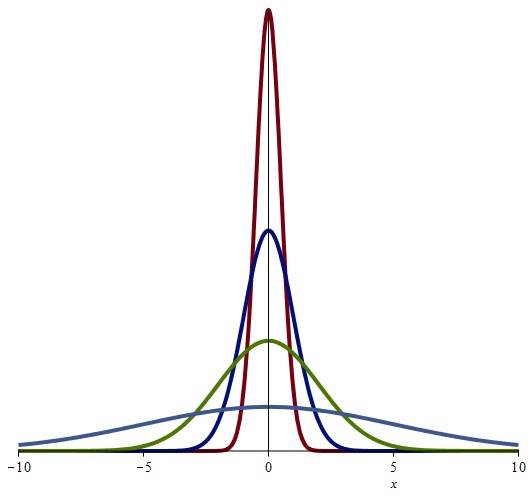
\includegraphics[width=0.4\textwidth]{images/normal_sd.png} 
 \qquad\qquad 
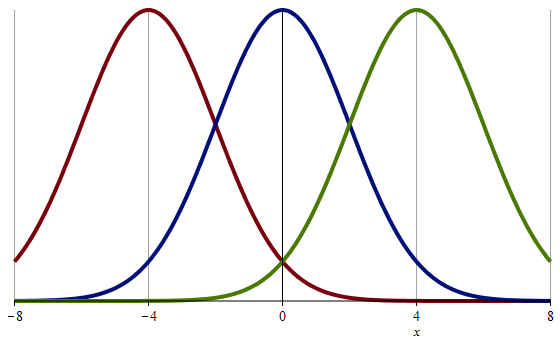
\includegraphics[width=0.4\textwidth]{images/normal_m.png}
\caption{Left: pdf of $\norm(0,\sigma^2)$ for $\sigma= 0.5, 1, 2, 5$. Right: pdf of $\norm(\mu,4)$ for $\mu=-4,0,4$. \label{normp}}
\end{figure}
The normal distribution is a familiar, symmetric ``bell-shaped curve'' centred on $\mu$.  The smaller $\sigma$ is the narrower the peak and therefore the greater likelihood of the random variable having a value close to the mean.  These features are clear in Figure~\ref{normp}. 
\end{n} 

\subsection{The Central Limit Theorem}

\ssn{The Central Limit Theorem}
The central limit theorem is the first big theorem of probability theory and plays a central role in applications. It's proof is beyond the scope of this course, and we will not even make a precise statement.  The idea however is important. 

\tcb
Consider a sequence of independent, identically distributed (i.i.d.) random variables $X_1, X_2, \dots$ each with mean $\mu$ and variance $\sigma^2$.  We know from \ref{wlln0} that the ``average of the first $n$''
 \[
   \bar{X}_n = \frac1n (X_1 + X_2 + \dots + X_n) 
 \]
has $\EE(\bar{X}_n) = \mu$ and variance $\var(\bar{X}_n) = \sigma^2/n$. 

The central limit theorem states that 
$$ \frac{ \bar{X}_n - \EE \bar{X}_n }{ \sqrt{\var(\bar{X}_n)} } \stackrel{\text{approx.}}{\sim} \norm(0,1)$$
for large $n$.
\etcb 

Note that there are many equivalent statements. Denote with $\Phi$ the cdf of the standard normal distribution, i.e.\ of $\norm(0,1)$, then
\begin{itemize}
    \item $\PP (\frac{ \bar{X}_n - \EE \bar{X}_n }{ \sqrt{\var(\bar{X}_n)} } \leq x ) \approx \Phi (x)$,
    \item $\PP \left( \sqrt{n} \frac{\bar{X}_n - \mu}{\sigma}  \leq x \right) \approx \Phi ( x )$,
    \item $\PP \left( \frac{\sum_{i=1}^n X_i - \EE \sum_{i=1}^n X_i}{\sqrt{\var(\sum_{i=1}^n X_i)}} \leq x \right) \approx \Phi ( x )$,
    \item $\PP \left( \frac{\sum_{i=1}^n X_i - n \mu}{\sqrt{n}\sigma} \leq x \right) \approx \Phi ( x )$,
    \item $\PP \left( a \leq \frac{\sum_{i=1}^n X_i - n \mu}{\sqrt{n}\sigma} \leq b \right) \approx \Phi ( b ) - \Phi(a)$.
\end{itemize}
\end{n}


%\ssn{Use of Central Limit Theorem}
%A practical application is that for large enough $n$, we can approximate $\bar{X}_n$ as having distribution $\norm(\mu , \sigma^2/n)$. 
%\end{n}

\ssn{Visualization of Central Limit Theorem}
Figure~\ref{fig:clt_plot} illustrates the application of the CLT for different sample sizes $n$ when applied to iid. Exponential rvs, $X_i\sim\text{Exp}(1)$ for $i=1,\ldots,n$. The expectation for this Exponential rv is $\mu=\EE{X_i}=\frac{1}{\lambda}=1$ and and its variance is $\var{X_i}=\frac{1}{\lambda^2} = 1$. As the sample size increases, we can see that the pdf for the sample mean, $f_{\bar{X}}(x)$ (solid line), becomes more symmetric and bell-like in shape until it is visually indistinguishable from the corresponding Normal approximation (dashed line) for the given sample size, i.e. $\bar{X}_n \stackrel{\text{approx.}}{\sim} \norm(1,\frac{1}{n})$ when $n$ is large.

\begin{figure}[!h]
    \centering
    \resizebox{\textwidth}{!}{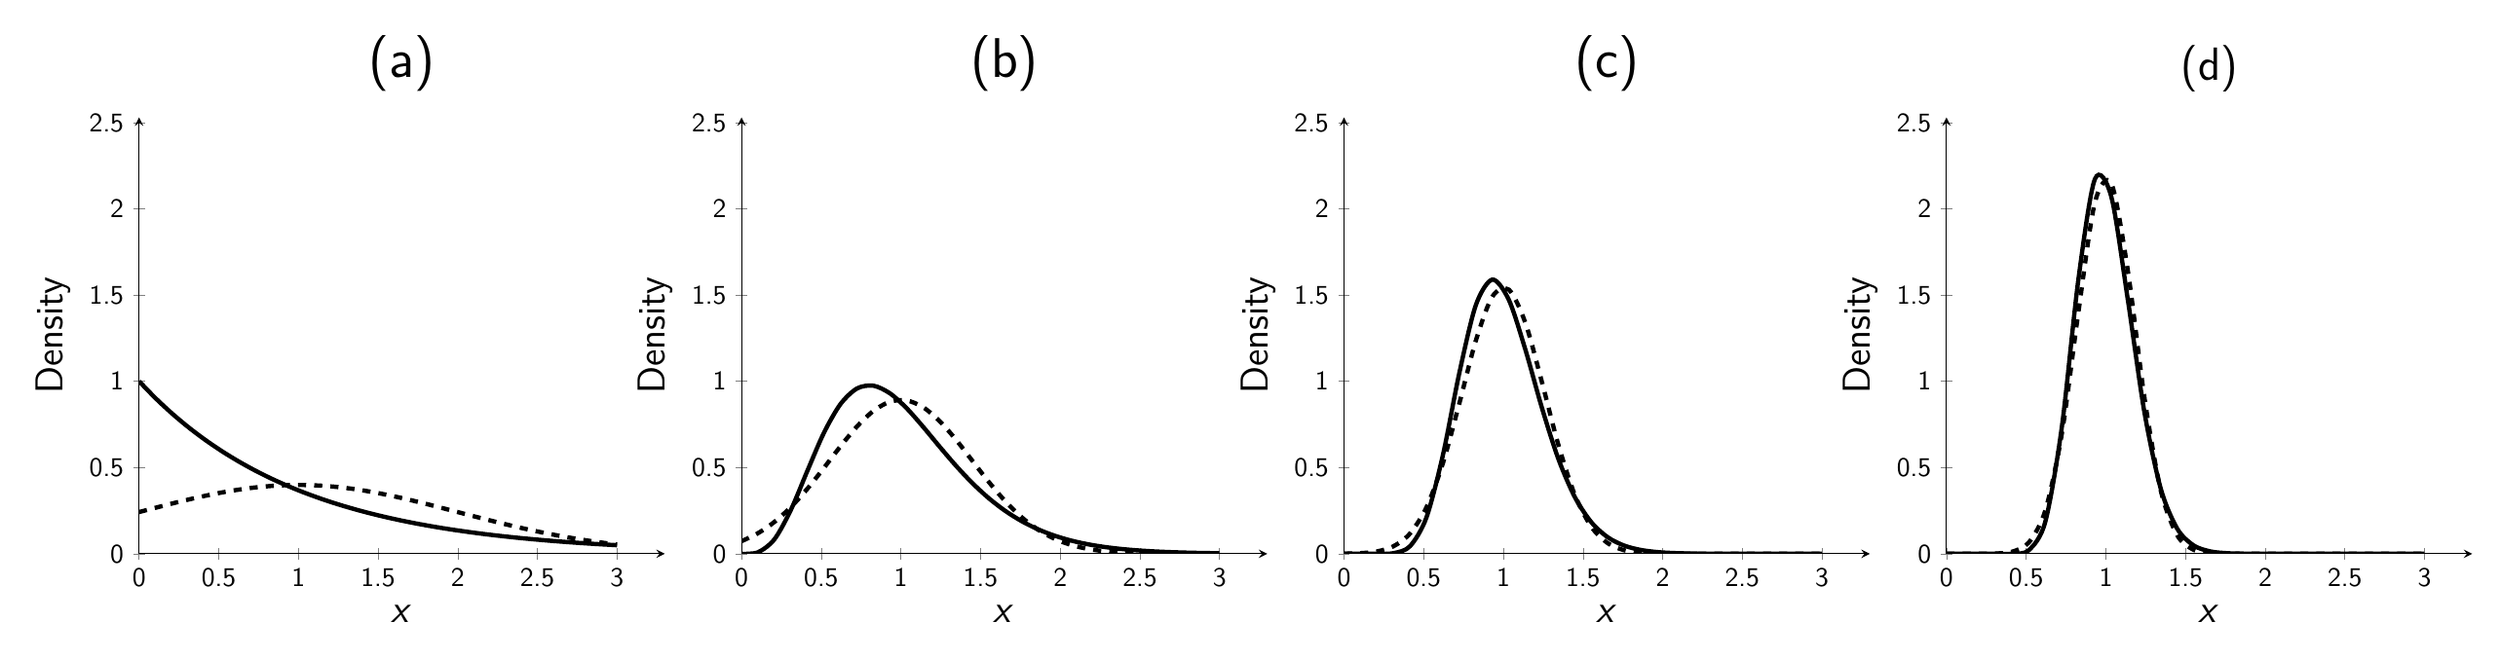
\begin{tikzpicture}[
    declare function={gamma(\z)=
    (2.506628274631*sqrt(1/\z) + 0.20888568*(1/\z)^(1.5) + 0.00870357*(1/\z)^(2.5) - (174.2106599*(1/\z)^(3.5))/25920 - (715.6423511*(1/\z)^(4.5))/1244160)*exp((-ln(1/\z)-1)*\z);},
    declare function={gammapdf(\x,\a,\b) = \b^\a * \x^(\a-1) * exp(-\x*\b) / (gamma(\a));},
    declare function={ExpCLTpdf(\x,\n) = gammapdf(\x*\n,\n,1)*\n;},
    declare function={gauss(\x,\m,\s) = exp(-(\x-\m)^2/(2*\s^2)) / (2.506628*\s);}
]

\begin{groupplot}[
    group style={rows=1,columns=4},
    axis lines=left,
    enlargelimits=upper,
    samples=30,
    xlabel = {\Large $x$},
    ylabel = {\Large Density},
    ymax=2.3,
    ymin=0,
    every axis plot/.append style={ultra thick}
]

\nextgroupplot[title = \huge (a)]
\addplot [smooth, domain=0:3] {ExpCLTpdf(x,1)};
\addplot [smooth, domain=0:3,dashed]
{gauss(\x, 1, sqrt(1/1))};

\nextgroupplot[title = \huge (b)]
\addplot [smooth, domain=0:3] {ExpCLTpdf(x,5)};
\addplot [smooth, domain=0:3,dashed]
{gauss(\x, 1, sqrt(1/5))};

\nextgroupplot[title = \huge (c)]
\addplot [smooth, domain=0:3] {ExpCLTpdf(x,15)};
\addplot [smooth, domain=0:3,dashed]
{gauss(\x, 1, sqrt(1/15))};

\nextgroupplot[title = \LARGE (d)]
\addplot [smooth, domain=0:3] {ExpCLTpdf(x,30)};
\addplot [smooth, domain=0:3,dashed]
{gauss(\x, 1, sqrt(1/30))};

\end{groupplot}
\end{tikzpicture}
} 
    \caption{Application of the Central Limit Theorem to independent Exponential ($\lambda=1$) random variables with sample sizes (a) $n=1$, (b) $n=5$, (c) $n=15$ and (d) $n=30$. Solid line: Probability density function for the sample mean, $f_{\bar{X}}(x)$. Dashed line: approximate Normal distribution.}
    \label{fig:clt_plot}
\end{figure}

\end{n}

\ssn{And now the bad news}
The problem with the normal distribution is that one cannot explicitly integrate the pdf.  We solve this in two stages. 
\begin{enumerate}[(A)] 
\item 
\tcb 
If $X \sim \norm(\mu, \sigma^2)$ then 
 \[
       Z =    \frac1\sigma ( X - \mu) 
 \]
 has $\norm(0,1)$ distribution. 
 \etcb 
 
 \noindent This process of using this transform is often referred to as ``calculating a $Z$ value''.
 \item We use a table of values  (or calculator, etc) to look up values for the cumulative distribution function of $\norm(0,1)$, a function that we normally denote by $\Phi$.  So 
\tcb   \[
     \Phi(z) =  
     \frac1{\sqrt{2\pi}}\int_{-\infty}^z e^{-\frac{x^2}{2}}\dd x.
  \]
 \etcb 
 
 \noindent 
 We then calculate for $a\leq b$: 
   \[ 
   \PP( a \leq Z \leq b) = \Phi(b) - \Phi(a). 
   \]
 For negative values of $z$ we use $\Phi(-z) = 1-\Phi(z)$.  
 A stripped down set of tables that will be enough for us is found in Tables \ref{ntable} and \ref{ntable2}
\end{enumerate}
\end{n}

\begin{table}[h]
\centering
\begin{tabular}{|c|cccccccccc|}
 \hline 
 $\Phi(z)$  & 0.0&0.1&0.2&0.3&0.4&0.5&0.6&0.7&0.8&0.9  \\ 
   \hline 
0+& .5000 & 
.5398 & 
.5793 & 
.6179 &
.6554 &
.6915 &
.7257 &  
.7580 & 
.7881 & 
.8159  \\
1+& .8413 &
.8643 &
.8849 &
.9032 &
.9192 &
.9332 &
.9452 &
.9554 &
.9641 &
.9713 \\
2+& .9772 &
.9821 &
.9861 &
.9893 &
.9918 &
.9938 &
.9953 &
.9965 &
.9974 &
.9981 \\
3+ & .9987 &
.9990 &
.9993 &
.9995 &
.9997 & .9998& .9998 & .9999 & .9999 & .9999 \\
\hline 
\end{tabular}
\caption{\label{ntable} Values of $\Phi(z)$ for $0 \leq z < 4$ in steps of $0.1$. (Use $\Phi(-z)=1-\Phi(z)$ for negative values.)}
\end{table}

\begin{table}[h]
\centering
\begin{tabular}{|c|cccccc|}
 \hline 
 $\Phi(z)=$ & 0.9000 & 0.9500 & 0.9750 & 0.9900 & 0.9950 &0.9990     \\
 $z=$ &   1.283 & 1.645 & 1.960 & 2.326 & 2.576 & 3.090 \\
 \hline 
\end{tabular}
\caption{\label{ntable2} Values of $z$ with particular useful values of $\Phi(z)$.}
\end{table}

\ssn{Example}  
Let $X$ be normally distributed with $\mu = 3$ and $\sigma = 2$.  Evaluate 
$\PP( 1 < X < 2)$.

Here 
 \[
    Z = \frac{X-\mu}{\sigma} = \frac{X-3}{2}.
 \]
So $X=1$ and $X=2$ correspond to $Z=-1$ and $Z=-1/2$ respectively. So we want
 \[
  \PP(-1 < Z < -1/2) = \Phi(-1/2) - \Phi(-1) = 
   ( 1 - \Phi(1/2)) - ( 1- \Phi(1)) \approx 0.1498. 
 \]
\end{n}



\sse
In Fig.\ \ref{normp}, identify which graph corresponds to which values of $\mu$ and $\sigma$. 
\end{e}

\sse 
Let $X$ be normally distributed with $\mu = 3$ and $\sigma = 2$.  Evaluate 
$\PP( 1 < X < 2)$.  
\end{e}



\ssn{Example} 
We are now in a position to answer the first motivating question: I toss a coin a million times; what is the probability that I get between 49.95\% and 50.05\% `heads'?  

The number of heads we get is a random variable $X$ binomial distribution with $n=10^6$ and $p=1/2$.  The binomial distribution is an average of $n$ Bernoulli trials (tossing a single coin and counting how many heads), each of which has expected value $p=1/2$ and variance $p(1-p) = 1/4$.  The expected value and variance of $X$ are thus 
 \[
 \EE(X)= np = 500,000;  \qquad \var(X) = \sigma^2 = np(1-p) = 250,000,   
 \]
(which are facts about the binomial distribution we knew previously). 
Also, $\sigma = 500$.  

Having a look at the Central Limit Theorem, we can rewrite the sought probability as
\begin{align*}
\PP ( 0.4995 \cdot n \leq X \leq 0.5005 \cdot n)
&= \PP ( \frac{ 0.4995 \cdot n - \EE X }{\sqrt{\var (X)}} \leq \frac{ X - \EE X }{\sqrt{\var (X)}} \leq \frac{ 0.5005 \cdot n - \EE X }{\sqrt{\var (X)}}
\\ &
= \PP ( \frac{ -500 \cdot n }{500} \leq \frac{ X - \EE X }{\sqrt{\var (X)}} \leq \frac{ 500 }{500}
\\ &
\approx \Phi(1)- \Phi(-1) 
\\ &
= 2 \Phi(1) - 1 
\\ &
\approx 0.682.
\end{align*}
However, since $X$ takes discrete values, while we are approximating with a continuous distribution, we might want to make a ``continuity correction'' to improve our result. 
  So e.g.\ we associate the discrete value of 499500 heads with the range $[499499.5, 499500.5]$ in the normal distribution. (You will not lose marks in this course if you neglect this and quite often we specifically ask you not to do this.)  
 Then our problem changes form whether $499500 \leq X \leq 5005$ to 
$ 499499.5 \leq X \leq 500500.5 $
 for our calculation, which changes the result to $2 \Phi( 1.001)-1$, which gives the same numerical result.


\noindent 
The transformation from $X$ values to $Z$ values is  
 \[
     Z = \frac1\sigma (X - \mu) = \frac1{500} (X - 500,000)
 \]
 and this takes $X=499499.5$ and $X=500500.5$ to something very close to $Z=-1$ and $Z=1$ respectively. 
 So the corresponding question about $Z$ is to find $\PP(-1 \leq Z \leq 1)$.  Thus our answer is 
  \[
   \Phi(1) - \Phi(-1) = \Phi(1) - (1-\Phi(1)) = 2 \Phi(1) - 1 \approx 0.682.
  \]
 (Useful rule of thumb: approximately 2/3 of a normal distribution is within one standard deviation of the mean.) 
 
I tried to check this answer with Wolfram alpha.   It gave me the following --- not sure how it added up lots of positive numbers and obtained something negative.  I guess this is why we use the normal approximation! 
\begin{figure}[h!] 
\centering
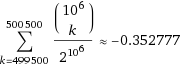
\includegraphics[]{images/wal.png}
\end{figure}
\end{n}

\ssn{Proposition}  \label{affnorm}
Let $X$ be a normal random variable with $\EE(X)=\mu, \var(X) =\sigma^2$.   Then given constants $a\not=0, b$ the random variable $Y=aX+b$ is also normally distributed with $\EE(Y)=a\mu +b$ and $\var(Y) = a^2 \sigma^2$. 
\begin{proof}
The fact that the expectation and variance are as claimed follows from general theory.  The verification that $Y$ is normal is a straightforward application of \S\ref{ltrrv}. (Exercise.) 
\end{proof}
We were implicitly assuming this result in the introductory reading. 
\end{n}

\ssn{Example: distribution of $Z^2$}
It is important in applications to understand the distribution of the square of a normally distributed random variable. Suppose that $Z$ is standard normal.   

Using the cumulative distribution trick again, 
 \[
 \PP( Z^2 \leq x ) = \PP( -\sqrt{x} \leq Z \leq \sqrt{z} ) 
  = 2 \PP( 0 \leq Z \leq \sqrt{z} ).  
 \]
Setting $X$ = $Z^2$ we therefore have 
 \[
   F_X(x) = \PP( X \leq \sqrt{x}) = \frac2{\sqrt{2\pi}} \int_0^{\sqrt{x}} e^{-z^2/2} \dd z
  \]
 and so 
 \[
  f_X(x)  = \frac{\dd}{\dd x} 
  \left(  \frac2{\sqrt{2\pi}} \int_0^{\sqrt{x}} e^{-z^2/2} \dd z  \right) = 
   \frac2{\sqrt{2\pi}} e^{-x/2} \frac{\dd}{\dd x} \sqrt{x} = 
    \frac1{\sqrt{2\pi}} x^{-1/2}  e^{-x/2}.
 \]
The fact that this is a constant times $x^{-1/2} e^{-x/2}$ means this must be the gamma distribution with $\alpha = \lambda = 1/2$. 
\end{n}

\ssn{The $\chi^2$ and other distributions (optional)}
Because of the Central Limit Theorem, a lot of basic statistics rests on normal distributions: data is often assumed to have come from sampling from a normal distribution unless there is evidence otherwise.  The $\chi^2$ distribution with $n$ degrees of freedom is precisely the sum of the squares of $n$ independent standard random variables. (So above we showed that $\chi^2(1) \sim \gamm(1/2,1/2)$.)   Other well-used distributions include the $F$-distribution which is (up to a scale) a quotient of two $\chi^2$ random variables and Student's t-distribution which measures the distribution of the mean of a sample from a normal distribution. 

Returning to $\chi^2$, let us try and understand $\chi^2(2)$.  If we have a unit normal random variable $X$ then for a small increment $\Delta x$ in $x$ we have
 \[
      \PP( x \leq X \leq x+ \Delta x) \approx f_X(x) \Delta x = 
       \frac1{\sqrt{2 \pi}} e^{-x^2/2} \Delta x.
 \]
If we have another independent normal random variable $Y$ then 
 \[
    \PP( x \leq X \leq x+ \Delta x \,\text{ and } \, 
     y \leq Y \leq y + \Delta y) \approx 
      \frac{1}{2 \pi} e^{-(x^2 + y^2)/2} \Delta x \, \Delta y.
 \]
Thus we have what we will soon call ``joint density function'' 
 \[
       f_{X,Y}(x,y)  = \frac1{2\pi}  e^{-(x^2+y^2)/2}
 \]
that can be integrated to calculate the probability of the ``random point'' $(X,Y)$ lying in a given area of the $(x,y)$-plane.

In particular, we can use this to calculate the cumulative distribution of $X^2+Y^2$ by converting to polar coordinates:
\begin{eqnarray*} 
     F_{X^2+Y^2}(t) &=&  \PP( X^2+Y^2 \leq t) \\
       &=& \frac1{2\pi}  \int_{r=0}^{\sqrt{t}} \int_{\theta=0}^{2\pi} 
         e^{-r^2/2} r \dd \theta \dd r \\
      &=&  \int_{r=0}^{\sqrt{t}} 
        r  e^{-r^2/2}  \dd r  = \left[ - e^{-r^2/2}   \right]^{\sqrt{t}}_0  = 1 - e^{-t/2}.
\end{eqnarray*} 
We recognise this (or we differentiate) to obtain the density function 
 \[
     f_{X^2+Y^2}(t) = \frac12 e^{-t/2}
 \]
and so  $\chi^2(2) \sim \expo(-1/2)$ or equivalently $\gamm(1, 1/2)$.

\bpr 
Follow the above reasoning to deduce that $\chi^2(3) \sim \gamm(3/2, 1/2)$. You will need to substitute $u=r^2$ in the final integral to obtain a result in terms of the $\Gamma$-function.   

For a further challenge, consider higher values of $n$. 
\epr %\\end{e}

\end{n} % was above \bpr

\subsection{Exercises and problems} 
 

\sse 
In the ``million tosses'' problem, how likely is it that at least 50.1\% of the tosses come down ``heads''.    (Ans: 0.0228)
\end{e}
 
\sse 
In Problem~\ref{chebex} you were asked to calculate a value of $n$ such that  the probability that the proportion of heads is within $0.01$ of $0.5$ is at least $0.95$. (The result was that it requires $n\geq 200,000$.) 

Use approximation by a normal distribution to estimate the value of $n$ needed for this to be true.  
 \end{e}
 
\sss 
The number $N$ of heads in $n$ tosses is binomial $(n, 1/2)$ and so has expected value $n/2$ and variance $n/4$. The proportion of heads is $X= N/n$ which thus has expected value $1/2$ and variance $1/(4n)$. The $Z$-transformation is thus 
 \[
       Z = \frac{ X - 0.5}{1/(2\sqrt{n})}.
 \]
From tables, $\Phi(2) \approx 0.975$ and so 
 \[
 \PP(-2 \leq Z \leq 2) \approx 0.95.
 \]
For $|X-0.5|\leq 0.01$ to translate into $|Z| \leq 2$ we require 
 \[
         \frac{0.01}{1/(2\sqrt{n})} \geq 2
 \]
or $n \geq 10,000$. 
\end{s}
 
 
 
\sse 
Adapt the statement and proof of \S\ref{ltrrv} to cover the case $a<0$.
\end{e}

\sss 
The correct statement is 
 \[
      f_{aX+b}(x) = \frac1{|a|} 
      f_X\left( \frac1a(x-b) \right) .
 \]
For the proof, remember that when you multiply n inequality by a negative number, the direction reverses. 
\end{s}

\sse 
Complete the proof of \S\ref{affnorm}. 
\end{e}


%%Week 07
\section{Several Random Variables}
\label{s9} 

%\ssn{Learning Outcomes}
%After studying this week you will be able to:
%\begin{itemize}
%\item calculate probabilities and marginal densities from joint densities;  
%\item use joint densities to solve some problems involving more than one random variable. 
%\end{itemize}
%\end{n}

\subsection{Joint densities}



\ssn{Motivating problems}
\begin{itemize}
\item How can we work with several random variables at once? 
\item A unit length, thin rod breaks in two places, each break independently uniformly distributed on $(0,1)$.  What is the probability that the breaks are more than distance $0.5$ apart? 
\item I choose five numbers in $[0,1]$ uniformly randomly. What is the expected position of the second smallest number? 
\end{itemize}
\end{n}



\ssn{Magic coins}
\begin{table}[h] 
\centering  \[  \arraycolsep=6pt\def\arraystretch{2.0} 
\begin{array}{|c|cc|}
 \hline 
   & X=H & X=T \\ 
  \hline
Y=H &  \frac4{12} & 
      \frac1{12}    \\
Y=T &  \frac2{12} & \frac5{12}  \\
\hline
\end{array} \quad 
\begin{array}{|c|cc|}
 \hline 
   & \PP(X=H)=\frac12 & \PP(X=T)=\frac12 \\
  \hline
\PP(Y=H)=\frac5{12} &  \frac4{12} & 
      \frac1{12}    \\ 
\PP(Y=T)=\frac7{12} &  \frac2{12} & \frac5{12}  \\
\hline
\end{array}
\] 
\caption{Pair of magic coins. (The numbers mean that e.g.\ the probability of both being T is $5/12$.) On the left the probability of all the outcomes is given. In the version on the right the ``marginal probabilities'' for $X$ and $Y$ have been added. \label{mc1}}
\end{table}

My two magic coins $X$ and $Y$ come down with probabilities as in the left-hand side of Table~\ref{mc1}; the four probabilities add up to $1$, as they should.   From that data, we can compute the probabilities that each of the coins separately comes down H or T by adding up each row and column; that information has been added to the table on the right.   But $\PP( \text{$X=H$ and $Y=H$}) \not= \PP(X=H)\, \PP(Y=H)$: the first coin and the second are not independent. 
\end{n}

\ssn{The discrete case}  \label{jdisc} 
Consider two discrete random variables $X,Y$ which for simplicity we assume take values in the non-negative integers $0,1,2,\dots$.   (Each may take infinitely many values (e.g.\ geometric or Poisson) or just a finite number of them (e.g.\ binomial).) 

\tcb 
The \emph{joint probability mass function} of $X,Y$ is 
 \[
      p_{X,Y}(x,y) = \PP(\text{$X=x$ and $Y=y$}). 
 \]
 \etcb 
 
 \noindent
To be valid, we need only to know that 
  \[
    0 \leq p_{X,Y}(x,y) \leq 1 \;\text{ for all $x,y$ } \quad \text{ and } \quad \sum_x \sum_y p_{X,Y}(x,y) = 1. 
   \] 
 
\tcb 
The \emph{marginal mass functions} of $X,Y$ are defined by 
 \[
     p_X(x) = \sum_y p_{X,Y}(x,y)  \quad \text{ and } \quad  p_Y(y) = \sum_x p_{X,Y}(x,y). 
 \]
 \etcb 
 
 \noindent
 They tell us the distribution of each variable, ignoring the other one. 
Clearly, one can extend the definitions to three or more random variables. 
\end{n}

\sse{} 
Prove that the joint mass function $p_{X,Y}$ satisfying the two conditions in \S\ref{jdisc} implies that the marginal distributions satisfy the conditions to be probability mass functions.  
\end{e}

\ssn{The continuous case}
For one continuous random variable $X$ we have a density function $f_X(x)$. It is such that in the limit as  $\Delta x \map 0$ we have 
 \[
    \PP( x \leq X \leq x + \Delta x ) = f_X(x) \Delta x. 
 \]

Two continuous random variables $X,Y$ can be thought of as defining a random point $(X,Y)$ in the plane. A continuous random variable is described by a probability density function $f_{X,Y}$ taking non-negative values so that in the limit as $\Delta x \map 0$ and $\Delta y \map 0$ we have 
 \[
    \PP( \text{$x \leq X \leq x + \Delta x$ and 
    $y \leq Y \leq y + \Delta y$}) = f_X(x,y) \Delta x \Delta y. 
 \]

With our usual convention that the density function is taken to be zero outside of the region where $(X,Y)$ takes values, we require that 
 \[
      \int \int_{\mathbb R^2} f_{X,Y}(x,y) \, \dd x \dd y = 1
 \]
One case is where $f_{X,Y}(x,y) = k$ for all points in some region $D$ in the plane and zero outside. 
This corresponds to choosing a point $(X,Y)$ uniformly randomly in the region $D$.  The constant in that case is $k= 1/\mathop{Area}(D)$ and the probability that $(X,Y)$ lies in a particular (sensibly-shaped) region  $A \subseteq D$ is 

\tcb
 \[
  \PP( (X,Y) \in A) = \frac{\mathop{Area}(A)}{\mathop{Area}(D)}.
  \]
\etcb 
\end{n}

\ssn{Example} 
Let $D$ be the disc of radius $R>0$ centred at the origin and suppose $(X,Y)$ is uniformly distributed in $D$.  Then the probability that $(X,Y)$ lies in the region of the disc given by $x>0$ is $1/2$ and the probability that it lies in the disc of radius $R/2$ centred at the origin is 
 \[
       \frac{\pi (R/2)^2}{\pi R^2} = \frac14. 
  \]
\end{n}

\sse 
A standard dartboard has a scoring area which is a disc of radius 170mm. Between radii of 99 and 107 mm there is an annulus where darts score ``treble''.  One twentieth of that region is the sought-after ``treble 20''.  (Google for a picture of a dartboard -- you are looking for the small red area about 100mm above the centre.)   If darts land uniformly distributed on the scoring area, what is the probability of a ``treble 20''? 
(Ans: 0.0028)
\end{e}

\sss
 The annulus between radii of 99 and 107 has area $\pi(107^2 - 99^2)$ sq mm.  Take one twentieth of that and divide through by the area of the whole board ($\pi 170^2$). 
\end{s}

\sse{} 
In the magic coins example, show that $\PP(X=H \st Y=H) = 4/5$ and compute some other conditional probabilities. 
\end{e}

 \sss 
 Substitute in to $\PP( X=H \text{ and } Y=H) = \PP(Y=H) \PP(X=H \st Y=H)$. 
 \end{s} 



\ssn{The beta distribution} 
We turn now to a related problem which introduces the important beta distribution.  This is not core for us (and so identifying occasions for its use, etc, will not be examined), it provides a good example and is worth being aware of. 
\end{n}

\ssn{Mathematical background}   \label{intfact}
Let $a,b$ be non-negative integers.  Then 
 \[
   I_{a,b} \stackrel{\text{def}}{=}  
   \int_0^1 x^{a-1} (1-x)^{b-1} \dd x = \frac{(a-1)! (b-1)!}{(a+b-1)!} = \frac{\Gamma(a) \Gamma(b)}{\Gamma(a+b)}. 
 \]
To establish this, first check with a trivial integration that $I_{a,1}= 1/a$. Then integrate by parts (differentiating the ``$x^{a-1}$'' term) to establish that 
 \[
     I_{a-1,b} = \frac{b-1}{a-1} I_{a,b-1}.
 \]
With this, we can compute $I_{a,2}$ for all $a$ and so on. 
Thus the two facts 
 \[
      I_{a,1}= \frac1a , \quad I_{a-1,b} = \frac{b-1}{a-1} I_{a,b-1}
 \]
determine $I_{a,b}$ for all positive integer values of $a,b$.  It is easy to check that 
 \[
    B(a,b) =  \frac{\Gamma(a) \Gamma(b)}{\Gamma(a+b)}    
 \]
satisfies the same properties and so is the same function.  (The function $B(a,b)$ is often called the ``beta function''.) 
\end{n}




\ssn{The Beta distribution}
Given that fact, we can define a family of random variables on $[0,1]$. We say that $X$ has a \emph{Beta distribution with parameters $\alpha, \beta \in \mathbb N$} if it has pdf
\[
    f_X(x) =   \frac{\Gamma(\alpha+\beta)}{\Gamma(\alpha) \Gamma(\beta)}  x^{\alpha-1}  (1-x)^{\beta -1}, \qquad x \in [0,1]. 
\]
We will concentrate on the case where $\alpha,\beta$ are positive integers but more generally, everything we have said is true if they are arbitrary positive real numbers. 
\end{n}

\ssn{A problem}
We will now consider the following problem. Consider $n$ points independently uniformly distributed on $[0,1]$. What can I say about where the $k$-th largest point is? 
\end{n}

\ssn{The case $n=2$} 
The first non-trivial instance of the problem is to ask for the distribution of 
 \[
  M_1  = \min(X_1,X_2), \quad M_2 = \max(X_1,X_2)
  \]
 where $X_1, X_2$ are independently uniformly distributed on $[0,1]$. 
 
 Let $\Delta x, \, \Delta y$ be small and consider the probability that $(M_1,M_2)$ lies in the small rectangle where $x \leq M_1 \leq x + \Delta x$ and $y \leq M_2 \leq y+\Delta y$.  We have  
  \[
    \PP(  \text{$x \leq M_1 \leq $ and $y \leq M_2 \leq y+\Delta y$}  ) = f_{M_1,M_2}(x,y) \Delta x \, \Delta y
\]
where $f_{M_1,M_2}(x,y)$ is the joint distribution function. 

We know that $M_1 \leq M_2$ always and so $f_{M_1,M_2}(x,y)=0$ if $x > y$.   If $x \leq y$ however there are two ways that we can have $M_1=x$ and $M_2=y$: either $X_1=x$ and $X_2=y$ or $X_1=y$ and $X_2=x$.  So we have
 \begin{multline*} 
 \PP( (M_1,M_2) \in [x, x+\Delta x] \times [ y,y+\Delta y] )\\  = \PP( (X_1,X_2) \in [x, x+\Delta x] \times [ y,y+\Delta y] ) + \PP( (X_1,X_2) \in [y, y+\Delta y] \times [ x,x+\Delta x] ). 
 \end{multline*} 
 Switching to density functions, still maintaining $x\leq y$ we have 
  \[
     f_{M_1,M_2} (x,y) \Delta x \Delta y 
      =  f_{X_1,X_2} (x,y) \Delta x \Delta y  +
       f_{X_1,X_2} (y,x) \Delta x \Delta y 
  \] 
 and so finally
  \[
     f_{M_1,M_2} (x,y) = \begin{cases}  
            2 &   \text{if $x \leq y$ and $0 \leq x,y \leq 1$}\\
            0 & \text{otherwise}
      \end{cases} 
  \]
Thus $(M_1, M_2)$ is uniformly distributed over the triangle $T$ with vertices $(0,0)$, $(0,1)$ and $(1,1)$ in the $(x,y)$ plane. 

We can also compute the marginal density $f_1(x)$ for the position of $M_1$.  The cumulative distribution $F_1(x)$ is
 \[
  F_1(x) =   \PP( \min(X_1,X_2) \leq x) = 
     \PP( \text{ $X_1=x$ or $X_2=x$}) = 1 - (1-x)^2
 \]
as one can see by drawing a picture. So 
 \[
     f_1(x) = F_1'(x) = 2(1-x). 
 \]
\end{n}

\sse{} 
Compute the density $f_2(x)$ for the position of $M_2$.  Find also $\EE(M_1)$ and $\EE(M_2)$.  (Solution: $f_2(x) = 2x$, $\EE(M_1) = 1/3$, $\EE(M_2) = 2/3$.) 
\end{e} 



\ssn{The general problem}
Let us now solve the problem of the probable location of the k-th smallest point of $n$ points $X_1, \dots , X_n$ independently, uniformly distributed on $[0,1]$.  Let $f_{k,n}(x)$ be the pdf of its location and let $M_k$ be the position of the $k$-th smallest particle  We know that to first order in $\Delta x$ we have 
 \[
   f_{k,n}( x) \Delta x = \PP( x \leq M_k \leq x + \Delta x).
 \]
We now calculate the probability on the right, neglecting and terms involving $(\Delta x)^2$ or higher powers. We do this in two stages.
 \begin{itemize}
     \item There needs to be a point in the interval $[x,x+\Delta x]$. Each point is in the interval with probability $\Delta x$ and there are $n$ points. Thus the probability of this is $n \Delta x$.    (Note: corrections involving two or more points in this interval would involve higher powers of $\Delta x$ and so are discounted.) 
     \item There need to be $k-1$ of the other $n-1$ points lying in the interval $[0,x]$.  This is a binomial distribution problem and the required probability is 
      \[
           \binom{n-1}{k-1} x^{k-1} (1-x)^{n-k}. 
      \]
      This is going to be multiplied by $n \Delta x$ and so any terms here involving $\Delta x$ can be neglected.  (For instance, the uncertainty as to whether one of the $n-k$ particles might actually lie in $[x, x+ \Delta x]$ can be neglected. 
 \end{itemize}
 
Combining these and cancelling $\Delta x$ we arrive at 
\[
    f_{k,n}(x) = \frac{n!}{(k-1)! (n-k)!} x^{k-1} (1-x)^{n-k}
 \]
which we recognise as a Beta distribution with parameters $\alpha=k$ and $\beta = n-k+1$. 
\end{n}

\begin{figure}[h] 
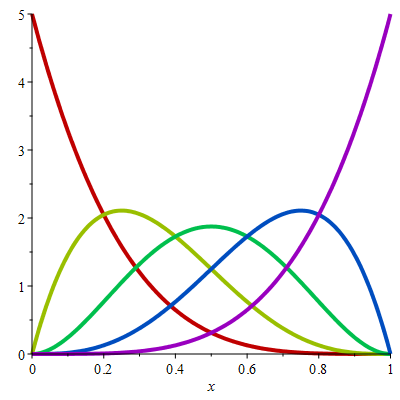
\includegraphics[width=0.45\textwidth]{images/beta5.png}\quad 
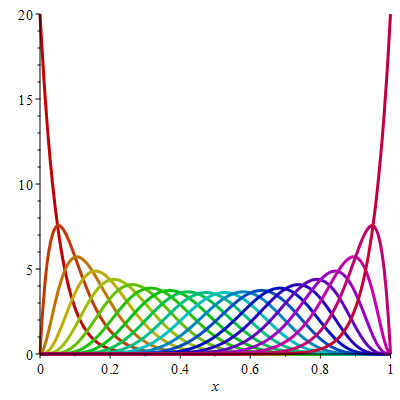
\includegraphics[width=0.45\textwidth]{images/beta20.png}
\caption{Pdf of position of $k$-th smallest of 5 (left) and 20 (right) independent, uniformly distributed numbers in $[0,1]$.  \label{kptpic}}
\end{figure}



\subsection{Exercises} 

\sse 
I toss a fair coin four times. Let $H$ be the number of heads I roll and let $C$ be the number of times (out of the three possible ones) that two consecutive coins tosses give the same result. 

Work out the $5 \times 3$ table of the joint probability mass function. From that compute the marginal distribution of $C$ and check that the marginal distribution of $H$ is binomial as you would expect.   Compute the expected value of $C$.  How could you compute the expected value of $C$ from the initial problem in your head? 
\end{e}

\sse
A unit length, thin rod breaks in two places, each break independently uniformly distributed on $[0,1]$. Let $a$ be a small number. Show that the probability that one of the three pieces into which the rod breaks has length less than $a$ is approximately $6a$ as $a \map 0$. 
\end{e}

\sss 
The relevant regions of the unit square are the four strips of width $a$ along each edge and a strip of width $\sqrt{a}$ around the $X_1 = X_2$ diagonal.  Ignoring overlaps (as $a \map 0$) they have a total area of $6 a$ 
\end{s}

\sse 
Compute the expected position of the $k$-th largest of $n$ independent, uniformly distributed numbers in $[0,1]$.  
\end{e}

\sss 
From the notes the pdf for the $k$th smallest of $n$ is 
\[
    f_{k,n}(x) = \frac{n!}{(k-1)! (n-k)!} x^{k-1} (1-x)^{n-k}. 
 \]
So its expected value is obtained by multiplying by $x$ and integrating: 
 \[
   \EE(X_{k,n}) = \int_0^1  \frac{n!}{(k-1)! (n-k)!} x^{k} (1-x)^{n-k}
   =  \frac{n!}{(k-1)! (n-k)!} \int_0^1   x^{k} (1-x)^{n-k}.
  \]
Using \S\ref{intfact} we evaluate the integral to be 
 \[
 \frac{n!}{(k-1)! (n-k)!} \, \frac{k! (n-k)!}{(n+1)!} = \frac{k}{n+1}.
 \]
\end{s}

\ssp 
Looking at the graphs in Figure~\ref{kptpic}, explain the following features, using mainly words rather than formulas. 
\begin{itemize}
\item Each picture is symmetric about the midpoint of the interval.
\item In the left-hand picture, the central blue-green graph is itself symmetric about the mid-point.
\item In both pictures, two of the graphs have non-zero values at one of the endpoints, but all the rest are zero at both end-points. 
\end{itemize}
\end{e}

\sss
\begin{itemize}
\item This is because the $k$-th smallest particle becomes the $k$-th largest particle if you reflect the interval in the mid-point. 
\item if there are an odd number $2k+1$ of particles, then the $k+1$-th particle reflects to itself under the symmetry just mentioned. 
\item The probability of having one particle in the interval $[0,\Delta t]$ is $n \Delta t$ as $\Delta t \map 0$.  So the corresponding distribution function approaches $n$ at the endpoints. But the probability of two points in such an interval is proportional to $(\Delta t)^2$ and so the distribution function must be zero at the end points. 
\end{itemize}
\end{s}



\subsection{Minimum and Maximum of Random Variables}

\ssn{Motivation}
In a large room are $n$ light bulbs. The owner is a little miserly and only changes them when all have burned out. How long is it till this has happened?
\end{n}

\ssn{Maximum of Random Variables}
Let $X_i$, $i \in \{1,2,\ldots, n \}$ be i.i.d. random variables with cdf $F_X$. 
Then
\begin{align*}
    F_{\max_i X_i} (x)
    &
    = \PP ( \max_i X_i \leq x)
    \\ &
    = \PP ( \text{each } X_i \text{ is } \leq x)
    \\&
    = \PP ( X_1 \leq x, X_2 \leq x, \ldots , X_n \leq x)
    \\ &
    = \Pi_{i=1}^n \PP (X_i \leq x)
    \\ &
    = F_X(x)^n
    .
\end{align*}
Depending on what distribution we assume $X_i$ to have, we get an explicit result. 

In the motivation above a standard choice would be to assume $X_i \sim \expo(\lambda)$, but note that it is not confined to this.
\end{n}

\ssn{Motivation}
In a production hall there are $n$ lamps. Regulations demand that when one of them faults, all have to be exchanged for new ones. How long is it till the next set of lamps gets installed?
\end{n}

\ssn{Minimum of Random variables}
Again, let $X_i$, $i \in \{1,2,\ldots, n \}$ be i.i.d. random variables with cdf $F_X$. 
Then
\begin{align*}
    F_{\min_i X_i} (x)
    &
    = \PP ( \min_i X_i \leq x)
    \\ &
    = 1 - \PP ( \min_i X_i > x)
    \\ &
    = 1 -  \PP ( X_1 > x, X_2 >x, \ldots , X_n > x )
    \\ &
    = 1 - \Pi_{i=1}^n (1- \PP ( X_i \leq x))
    \\ &
    = 1 - (1- F_X(x))^n
    .
\end{align*}
If we once more do our canonical choice of saying that the life of lamps is exponentially distributed to some parameter $\lambda>0$, then this simplifies for $x>0$ to
\begin{align*}
    F_{\min_i X_i} (x)
    &
    = 1 - ( 1 - (1 - e^{-\lambda x}))^n
    %\\&
    = 1- (e^{- \lambda x})^n
    %\\&
    = 1 - e^{-(n\lambda) x}.
\end{align*}
This means that the minimum of i.i.d. exponential random variables is again exponentially distributed with $\min_i X_i \sim \expo(n\lambda)$.
\end{n}


\subsection{Convolution/Sum of Random Variables}

\ssn{Motivation}
A shop has only $2$ items of some product in stock. The time till the next customer wants to buy this product is exponentially distributed to some parameter $\lambda > 0$. What is the distribution of the time when both items got sold?

\

Since the first product gets sold after an exponential random variable and then we again have to wait till the time given by another independent exponential random variable has past, we want to know the distribution of the sum of two exponential random variables.
\end{n}

\ssn{Derivation for discrete random variables}
Let $X$ and $Y$ be two independent discrete random variables. Because they are discrete, we can partition the universal set into the sets $\{ Y=y \}$ for $y$'s being all the values $Y$ can take. Thus we obtain
\begin{align*}
    \PP(X+Y=k)
    &
    = \PP (X=k-Y)
    \\ &
    = \sum_y \PP(\{X=k-Y\} \cap \{ Y = y \} )
    \\ &
    = \sum_y \PP (X=k-y, Y=y )
    \\ &
    = \sum_y \PP (X=k-y) \PP (Y=y),
\end{align*}
which we can rewrite with respect to the mass function as
$$ p_{X+Y}(k) = \sum_y p_X(k-y) p_Y(y).$$
\end{n}

\ssn{Theorem} \label{thm:X+Y}
\
\tcb
Let $X$ and $Y$ be two independent random variables. If they are discrete then
$$ p_{X+Y}(k) = \sum_y p_X(k-y) p_Y(y)$$
and if they are continuous then
$$f_{X+Y}(z) = \int_\RR f_X(z-y) f_Y(y) dy.$$
\etcb
\end{n}

\ssn{Example}
As a first very simple example let us calculate the distribution of the sum of two independent $\bern(p)$ rv's. We already know that the result should be a $\bino(2,p)$, but this is agread way of checking that our calculation is correct. Since both $X$ and $Y$ only take values in $\{0,1\}$, we have
$$ p_{X+Y} (k) 
= \sum_{y=0}^1 p_X(k-y) p_Y(y)
= \PP(X= k) \PP(Y=0) + \PP(X=k-1) \PP (Y=1).
$$
Because it is easy to see that values for $k$ outside of $\{0,1,2\}$ will result in probability of $0$, we only need to concern ourselves with
\begin{align*}
    k=0:& \quad p_{X+Y}(0) = \PP(X=0)\PP(Y=0) + \PP(X=-1)\PP(Y=1) = (1-p)^2
    ,\\
    k=1:& \quad p_{X+Y}(1) = \PP(X=1)\PP(Y=0) + \PP(X=0)\PP(Y=1) = 2p(1-p)
    ,\\
    k=2:& \quad p_{X+Y}(2) = \PP(X=2)\PP(Y=0) + \PP(X=1)\PP(Y=1) = p^2
    .
\end{align*}
This can also be written as $p_{X+Y}(k) = \binom{2}{k} p^k (1-p)^{n-k}$, which is exactly the desired $\bino(2,p)$ distribution.
\end{n}

\ssn{Example}
Assume that $X,Y \sim \norm(0,1)$ and independent. What is the distribution of $X+Y$? Let us start with the calculation:
\begin{align*}
    f_{X+Y}(z)
    &
    = \int_\RR f_X(z-y) f_Y(y) dy
    %\\ &
    =
    \int_\RR \left( \frac{1}{\sqrt{2 \pi}} \right)^2 e^{- \frac{ (z-y)^2}{2}} e^{- \frac{y^2}{2}} dy
    %\\ &
    = \int_\RR \frac{1}{2\pi} e^{- \frac{ z^2 - 2zy + 2 y^2}{2}} dy
    .
\end{align*}
Now we stand in front of the problem of getting rid of this integral. As mentioned before, there is no primitive that we can use. Hence, we have to resort to another tactic. Looking at the integral we notice that it still looks very much like the density of a general normal distribution. If it was a general normal distribution, then the integral over the density function would be equal to $1$ and would therefore disappear. 

So let us try this. Since $y$ is our integration variable, we need the density to look like $\frac{1}{\sqrt{2 \pi}} e^{- \frac{(y-\mu)^2}{2 \sigma^2}}$. Since there is a factor of $2$ in front of $y^2$, we have to choose $\sigma^2 = \frac12$, which means that we now have $\frac{y^2 -yz + \frac12 z^2}{2 \cdot \sigma^2}$ in the exponent. Furthermore choosing $\mu = \frac12 z$ this becomes $\frac{(y- \mu)^2 + \frac14 z^2}{2 \sigma^2}$. This is not exactly a normal density, but everything differing from the density of $\norm(\mu,\sigma^2)$ are just constants in regard to the integration variable $y$ and hence can be put in front of the integral.

Putting that together we obtain
\begin{align*}
    f_{X+Y}(z)
    &
    = \int_\RR \frac{1}{2\pi} e^{- \frac{ z^2 - 2zy + 2 y^2}{2}} dy
    \\ &
    = \int_\RR \frac{1}{\sqrt{2\pi 2}}\frac{1}{\sqrt{2\pi \frac12}} e^{- \frac{(y-\frac12 z)^2 + \frac14 z^2}{2 \frac12}} dy
    \\ &
    = \frac{1}{\sqrt{2\pi 2}} e^{- \frac{z^2}{2 \cdot 2}} \int_\RR \frac{1}{\sqrt{2\pi \sigma^2}} e^{- \frac{(y-\mu)^2 }{2 \sigma^2}} dy
    \\&
    = \frac{1}{\sqrt{2\pi 2}} e^{- \frac{z^2}{2 \cdot 2}} \cdot 1
    .
\end{align*}
As we can see here, this again is the pdf of a normal distribution, namely of $\norm(0,2)$. I.e. $X+Y \sim \norm(0,2)$.
\end{n}

\ssn{Theorem} \ \\
The sum of two independent normal random variables is again normally distributed:
\tcb
Let $X \sim \norm( \mu_X, \sigma_X^2)$ and $Y \sim \norm(\mu_Y, \sigma_Y^2)$ be independent. Then
$$ X+Y \sim \norm ( \mu_X + \mu_Y, \sigma_X^2 + \sigma_Y^2).$$
\etcb
\end{n}

\ssn{Example}
Now we consider the case of $X$ and $Y$ being $\unif (1,5)$ distributed and independent. As always we start by writing down the general formula and inserting the density functions:
$$ f_{X+Y}(z)
= \int_\RR f_X (z-y) f_Y(y) dy
= \int_\RR \frac{1}{5-1} \1_{\{ z-y \in [1,5] \}} \frac{1}{5-1} \1_{\{ y \in [1,5] \}} dy
. $$
Because $y$ is the integration variable we rewrite the first indicator function to $\1_{\{ z-y \in [1,5] \}} = \1_{\{ y \in [z-5,z-1] \}}$. What those indicators mean is that when either of them is $0$ we integrate nothing. If both are $1$, we integrate. Hence, our area of integration is the intersection of the intervals $[z-5,z-1]$ and $[1,5]$ from the indicator functions. Thus, we have to find out how large those intersections are for all values of $z$. To this end, it is a nice approach to first think about the values of $z$ where the behaviour of the length of intersection changes. The first such value is $z=2$, since for smaller $z$ they do not intersect, while for larger $z$ they do. Similarly for $z=10$. Finally for $z=6$ both intervals are equivalent. So, we do a case analysis between those points. We get
\begin{align*}
    f_{X+Y}(z) 
    &
    = \left\{ \begin{array}{ll}
        \frac{1}{16} \int_\RR 0 dy, & z < 2 \\
        \frac{1}{16} \int_\RR \1_{\{ y \in [1,z-1] \} } dy, & 2 \leq z \leq 6 \\
        \frac{1}{16} \int_\RR \1_{\{ y \in [z-5,5] \} } dy, & 6 \leq z \leq 10 \\
        \frac{1}{16} \int_\RR 0 dy, & 10 < z 
    \end{array} \right.
    = \left\{ \begin{array}{ll}
        0, & z < 2 \\
        \frac{1}{16} (z-2), & 2 \leq z \leq 6 \\
        \frac{1}{16} (10-z), & 6 \leq z \leq 10 \\
        0, & 10 < z 
    \end{array} \right.
    .
\end{align*}
As a sanity check, we compute the integral of this pdf and confirm that it yields $1$:
\begin{align*}
    \int_\RR f_{X+Y}(z) dz
    &
    = \int_2^6 \frac{1}{16} (z-2) dz + \int_6^10 \frac{1}{16} (10-z) dz
    \\&
    = \frac{1}{16} \left[ \frac12 z^2 - 2 z \right]_2^6 + \frac{1}{16} \left[ 10 z - \frac12 z^2 \right]_6^10
    \\ &
    = \frac{1}{16}( 18 - 12 - 2 + 4) + \frac{1}{16}( 100 - 50 - 60 + 18)
    \\ &
    = 1.
\end{align*}
\end{n}

\ssn{Some further sums} \label{DistrSumsStandard}
There are even more distributions where, when you sum up multiple random variables, you get another standard distribution. Examples are:
\begin{enumerate}[(i)]
\item
$X\sim \bino(n_X,p)$, $Y \sim \bino(n_Y,p)$ $\Rightarrow$ $X+Y \sim \bino(n_X+n_Y,p)$,
\item
$X\sim Expo(\lambda)$, $Y\sim Expo(\lambda)$ $\Rightarrow$ $X+Y \sim Gamma(2,\lambda)$,
\item
$X\sim Gamma (\alpha, \lambda)$, $Y\sim Gamma (\beta, \lambda)$ $\Rightarrow$ $X+Y \sim Gamma (\alpha + \beta, \lambda)$,
\item
$X\sim \norm (\mu_1, \sigma_1^2)$, $Y\sim \norm (\mu_2, \sigma_2^2)$ $\Rightarrow$ $X+Y \sim \norm (\mu_1 + \mu_2, \sigma_1^2 + \sigma_2^2 )$,
\item
$X\sim Poisson(\lambda_1)$, $Y\sim Poisson (\lambda_2)$ $\Rightarrow$ $X+Y \sim Poisson (\lambda_1 + \lambda_2)$,
\item
$X\sim Expo(\lambda_1)$, $Y\sim Expo(\lambda_2) $ $\Rightarrow$ $\min \{ X,Y \} \sim Expo (\lambda_1 + \lambda_2 )$
.
\end{enumerate}
\end{n}

\sse
Prove the statements $(i),(ii),(iii),(v)$ from the list in \ref{DistrSumsStandard}.
\\
(\textit{Hint}: For distributions that do not take values on $\RR$, or $\ZZ$, first think about which values they and their sums can take.)
\end{e}

\sse
Derive a formula similar to the one in Theorem \ref{thm:X+Y} for the distribution of $X-Y$.
\end{e}

\sss
If $X$ and $Y$ are discrete then
$$ p_{X-Y}(k) = \sum_y p_X(k+y) p_Y(y)$$
and if they are continuous then
$$f_{X-Y}(z) = \int_\RR f_X(z+y) f_Y(y) dy.$$
\end{s}




%%Week 08
\section{Transformations, Chebyshev's inequality and LLN}
\subsection{Transformations}

\ssn{Motivating problem}

You are working in a laboratory and know from experience that the result $X$ of some experiment is uniformly distributed in the range $[1,2]$. For a public presentation you want to do this experiment in a larger scale. You plan to triple the size, i.e.\ the new result $Y$ will be $Y=3 \cdot X$. To implement some safety precautions you need to know the distribution of $Y$. \\
What is the pdf of $Y$ here?

\end{n}

\ssn{Example}

Let $X \sim \unif(1,2)$ and $Y:= 3 \cdot X$. What is the pdf $f_X$?

We know from Proposition \ref{PropCdfPdf} that $f_Y(y) = \partial_y F_Y (y)$, hence we can just concentrate on finding $F_Y$.
First, we have a look at the definition $F_Y(y) = \PP (Y \leq y)$. Here we notice, that since $Y= 3X$, we can simply replace it to obtain $\PP(Y \leq y) = \PP(3X \leq y)$. Doing the equivalent transform of dividing both sides of the inequality by 3 we have $\PP(3X\leq y)= \PP(X \leq y/3)$. Notice that this is the cdf of $X$, which we know to be
$$F_X(x)= \int_{-\infty}^x \1_{\{x \in [1,2]\}} dx
= \left\{ \begin{array}{ll}
0,\quad & x < 1 \\
x-1, \quad & 1 \leq x \leq 2 \\
1, \quad & 2 < x.
\end{array}
\right.$$
Putting this together we have
\begin{align*}
F_Y(y)
&
= \PP(Y\leq y)
%\\ &
= \PP(3X \leq y)
%\\ &
= \PP \Big(X \leq \frac{y}{3} \Big)
%\\ &
= F_X \Big(\frac{y}{3} \Big)
\\ &
= \left\{ \begin{array}{ll}
0,\quad & y/3 < 1 \\
y/3-1, \quad & 1 \leq y/3 \leq 2 \\
1, \quad & 2 < y/3.
\end{array}
\right. \quad
%\\ &
= \left\{ \begin{array}{ll}
0,\quad & y < 3 \\
y/3-1, \quad & 3 \leq y \leq 6 \\
1, \quad & 6 < y.
\end{array}
\right.
\end{align*}
Differentiating, we get $f_Y(y) = \partial_y F_Y(y) = \frac13 \1_{\{ y \in [3,6] \} }$, i.e.\ $Y$ is uniformly distributed on $[3,6]$.

\


\end{n}

\ssn{Theorem}


We did the last example for a quite simple transformation and a quite simple distribution. Can we do this in general?

Let us assume that now we are given the pdf of $X$, denoted by $f_X$ and that $Y:= g(X)$ for some function $g$. We can say the following.

\tcb
Let $X$ be a continuous random variable with given pdf $f_X$ and let $g: \RR \to \RR$ be such that its inverse $g^{-1}$ exists (i.e.\ there exists a function $g^{-1}$ such that $g^{-1}(g(x)) = x$), is differentiable and monotone increasing where $f_X$ is positive. Define $Y$ as $Y:= g(X)$. Then
$$f_Y(y) 
= f_X(g^{-1}(y))  \cdot (g^{-1})'(y).
$$
\etcb

\begin{proof}
We do the exact same calculation as above. In detail it is
\begin{align*}
F_Y(y)
&
= \PP(Y\leq y)
%\\ &
= \PP(g(X) \leq y)
%\\ &
= \PP (g^{-1}(g(X)) \leq g^{-1}(y))
%\\ &
= \PP (X \leq g^{-1}(y))
%\\ &
= F_X (g^{-1}(y)),
\end{align*}
where we used that applying the inverse of $g$ on both sides gives an equivalent statement. Finally, we differentiate to obtain
\begin{align*}
f_Y(y)
&
= \partial_y F_Y(y)
\\&
= \partial_y F_X( g^{-1}(y))
\\ &
= (F_X)'(g^{-1}(y)) \cdot (g^{-1})'(y)
\\ &
= f_X(g^{-1}(y)) \cdot (g^{-1})'(y),
\end{align*}
where the chain rule was applied.
\end{proof}

Now let us have a look at two examples where $g$ does not have an increasing inverse.

\end{n}

\ssn{Example}

Let $X \sim Exp(\lambda)$, $g(x)= -a x$ for some $a > 0$ and $Y:=g(X)$.
\\
We can still use the basic calculation from above. However, the step where we formally applied the inverse of $g$ requires closer attention.
\begin{align*}
F_Y(y)
&
= \PP(Y\leq y)
%\\ &
= \PP(-aX \leq y)
\end{align*}
Here it becomes obvious that the calculation does not go the exact same way. Instead we obtain
$$ \PP(-aX \leq y) = \PP\Big(X \geq -\frac{y}{a}\Big).$$
Continuing our calculation with this slightly changed step and using that single points have probability 0, we get
\begin{align*}
F_Y(y)
&
=\PP\Big(X \geq -\frac{y}{a}\Big)
%\\&
= 1 - \PP\Big(X < -\frac{y}{a}\Big)
= 1 - \PP\Big(X < -\frac{y}{a}\Big)
= 1 - F_X\Big( -\frac{y}{a}\Big)
.
\end{align*}
Now we again can differentiate to obtain that
\begin{align*}
f_Y(y)
&= \partial_y F_Y(y)
= \partial_y \Big(1-F_X\Big(-\frac{y}{a}\Big)\Big)
= \frac1a f_X\Big(-\frac{y}{a}\Big)
= \left\{ \begin{array}{ll}
0, \quad & -\frac{y}{a} < 0 \\
\frac1a \lambda e^{-\lambda (-\frac{y}{a})}, \ & 0 \leq -\frac{y}{a}
\end{array} \right.
\\ &
= \left\{ \begin{array}{ll}
0, \quad & y > 0 \\
\frac{\lambda}{a} e^{\frac{\lambda}{a} y}, \ & 0 > y.
\end{array}
\right.
\end{align*}
Note that this is not an exponential distribution, since its mass is on the negative axes.

\end{n}

\ssn{Example}

As a final example, we have a look at what happens, if $g$ is not invertible. For this, let $g(x)= x^2$, $X \sim \unif([-1,2])$ and $Y:= g(X)$, i.e.\ $Y:= X^2$ and $F_X(x) = \frac13 (1+x) \1_{\{x \in [-1,2]\}} + \1_{\{x > 2\}}$. Starting as usual, we have
$F_Y(y)
= \PP ( X^2 \leq y ).$ Here we see the problem, that we cannot invert, since left from $0$ the inverse is $-\sqrt{\cdot}$, while on the right it is $\sqrt{\cdot}$. Instead, we find the equivalent formulation $\vert X \vert \leq \sqrt{y}$. However, we need to require for this that $y \geq 0$. Because $X^2 \geq 0$, this is no problem and just means that $F_Y(y) =0$ for all $y<0$. Collecting all of that, we progress to
$$ F_Y(y) 
= \PP ( X^2 \leq y ) 
= \PP ( \vert X \vert \leq \sqrt{y}) \1_{\{y \geq 0\}}
= \PP ( -\sqrt{y} \leq X \leq \sqrt{y}) \1_{\{y \geq 0\}}
.
$$
Replacing the probability with the cdf this reads as
$$ F_Y(y)
= \PP ( -\sqrt{y} \leq X \leq \sqrt{y}) \1_{\{y \geq 0\}}
= (F_X(\sqrt{y})-F_X(-\sqrt{y}))\1_{\{y \geq 0\}}
.
$$
Now we can use the explicit expression for $F_X$ from above to get
\begin{align*}
F_Y(y)
&
=
\left[ \frac13 (1+\sqrt{y}) \1_{\{\sqrt{y} \in [-1,2]\}} + \1_{\{\sqrt{y} > 2\}} - \frac13 (1-\sqrt{y}) \1_{\{-\sqrt{y} \in [-1,2]\}} - \1_{\{-\sqrt{y} > 2\}} \right] \1_{\{y \geq 0\}}
,
\end{align*}
which looks quite intimidating. However, in a first step we can simplify it, by removing all cases where $\sqrt{y}$ would have to be negative and as a second step, we split it up into the disjoint cases $\sqrt{y} \in [0,1]$, $\sqrt{y} \in [1,2]$ and $\sqrt{y} > 2$. Thus, we have
\begin{align*}
F_Y(y)
&
=
\left[ \frac13 (1+\sqrt{y}) \1_{\{\sqrt{y} \in [0,2]\}} + \1_{\{\sqrt{y} > 2\}} + \frac13 (\sqrt{y}-1) \1_{\{\sqrt{y} \in [0,1]\}} - 0 \right] \1_{\{y \geq 0\}}
\\ &
=
\left\{ \begin{array}{ll}
0, \quad & y < 0 \\
\frac13 (1+\sqrt{y}) + \frac13 (\sqrt{y}-1), \quad & 0 \leq \sqrt{y} \leq 1\\
\frac13 (1+\sqrt{y}), \quad & 1 < \sqrt{y} \leq 2 \\
1, \quad & 2 < \sqrt{y}
\end{array}
\right.
\\ &
=
\left\{ \begin{array}{ll}
0, \quad & y < 0 \\
\frac23 \sqrt{y}, \quad & 0 \leq y \leq 1\\
\frac13 (1+\sqrt{y}), \quad & 1 < y \leq 4 \\
1, \quad & 4 < y
\end{array}
\right.
.
\end{align*}
A quick sanity check is, whether this is actually a non-decreasing function as it should be. Since every single part is non-decreasing, we only need to have a look at the border cases $y=0,1,4$ which all turn out to be fine.

So finally, we only have to differentiate to obtain $f_Y$. Doing so we get
\begin{align*}
f_Y(y)
= \partial_y F_Y(y)
= \left\{ \begin{array}{ll}
0, \quad & y < 0 \\
\frac{1}{3 \sqrt{y}}, \quad & 0 \leq y \leq 1\\
\frac{1}{6 \sqrt{y}}, \quad & 1 < y \leq 4 \\
0, \quad & 4 < y
\end{array}
\right.
.
\end{align*}

\end{n}


\subsection{Exercises and problems}

\sse 
The random variable $X \sim \gamma(2,\lambda)$ and $Y:= \ln (X)$. Find the pdf $f_Y$. \\ (Ans.: $f_Y(y) = \frac{\lambda^2}{2} e^y e^{-\lambda e^y} \1_{\{y > 0\}}$ )
\end{e}

\sse{}
Show that for any continuous random variable $X$ it is true that $F_X(X) \sim \unif(0,1)$. 
\end{e}

\ssp{}
Let $X$ have any continuous distribution and let $Y \sim \unif(0,1)$. Show that $Z:= F_X^{-1} (Y)$ has the same distribution as $X$, i.e.\ that $F_Z = F_X$.
\end{e}

\sse{}
Let $X \sim \expo(\lambda)$.  Compute $F_Y$ for $Y:= X^2$.   (Ans: $(1-e^{-\lambda \sqrt{y}}) \1_{\{ y \geq 0 \}}$) 
\end{e}



\subsection{Chebyshev's Inequality and the Law of Large Numbers}

\ssn{Theorem (Chebyshev's inequality)}
Let $X$ be a random variable with expected value $\EE(X)=\mu$ and (finite) variance $\var(X)$. Then for every positive number $a$ we have 
\[
    \PP( | X-\mu| \geq a) \leq \frac{\var(X)}{a^2}.
\]
\begin{proof}
Rearrange the inequality in the form 
\[
      \var(X) \geq \PP( | X-\mu| \geq a) a^2. 
 \]
If you think about this, you may come to the conclusion that this is almost ``obvious''.  Let us write down a proof anyway. 

Calculate $\var(X)$ using the law of total probability for expectation'' conditioning on $|x-\mu| \geq a$ we have 
\[
  \var(X) = \EE( (X - \mu)^2 \st |x-\mu| \geq a ) \PP( |x-\mu| \geq a) 
 +  \EE( (X - \mu)^2 \st |x-\mu| <  a ) \PP( |x-\mu| < a).
\]
Both terms on the right-hand side are positive and the first term is greater than or equal to $a^2 \PP( |x-\mu| \geq a)$. 
\end{proof}
\end{n}

\ssn{Theorem (The weak law of large numbers)}
Consider an infinite sequence of independent, identically distributed random variables as in \S\ref{wlln0}.  Then for any $a>0$ we have 
 \[
     \PP( A_n - \mu \geq a ) \map 0 \; \text{as $n \map \infty$.}
 \]
 \begin{proof}
 Chebyshev's inequality applied to $A_n$ tells us that 
  \[
     \PP( | A_n - \mu | \geq a) \leq \frac{\var(A_n)}{a^2} = \frac{\var(X)}{a^2 n}
  \]
  which tends to zero as $n$ tends to infinity. 
 \end{proof}
\end{n}

\ssn{Discussion} 
The weak law of large numbers closes a circle. We defined (not really in the  mathematical sense) what we mean by the probability of a coin coming down heads being $1/2$ by saying that if we tossed it very many times, we would expect to get heads half the time.  The theorem we just proved says something exact about the situation: given a ``tolerance'' $a$, however small it may be, we can make the probability of the proportion of heads differing from $1/2$ by more than $a$ as small as we like by tossing the coin enough times. 
\end{n}

\ssn{Example}
Lets return to one of our motivating examples: what is the expected number of pairs of consecutive heads if you toss a coin $n$ times? 

Let $X_j$ for $1 \leq j \leq n-1$ be the random variable that takes the value 1 if the $j$-th and 
$(j+1)$-th tosses are both heads and 0 otherwise.   
Each of the $X_j$ separately has expected value $1/4$ since that is the probability that two coins both come down heads.   

The number we are interested in is the expected value of $\sum_{j=1}^{n-1} X_j$.  So 
 \[
  \EE\left( \sum_{j=1}^{n-1} X_j \right) = \sum_{j=1}^{n-1} \EE(X_j) = \frac{n-1}4. 
 \]
 
 Here,  $X_j$ and $X_{j+1}$ here are not independent. It is tempting to think that we would need independence to add expectations --- but we don't! 
 \end{n}





\ssp \label{chebex}
Use Chebyshev's inequality to to find a value of $n$ such that if you toss a coin $n$ times the proportion of heads will be within 0.01 of 0.5 with probability at least 0.95. 
\end{e}

\sss 
The number of heads $N$ in $n$ tosses is binomial $(n, 1/2)$.This has expected value $n/2$ and variance $n/4$. The proportion of heads is $X = N/n$ which thus has expected value $0.5$ and variance $1/(4n)$. 

Substituting into Chebyshev's inequality,
 \[
   \PP( |X-\frac12| \geq 0.01 ) \leq \frac{1/(4n)}{(0.01)^2}.
 \]
Solving, we require $n \geq 50,000$. 
\end{s}

\sse{}  Let $X \sim \bino(n,p)$ and $Y \sim \bino(m,p)$ be independent. Then $X+Y \sim \bino(n+m, p)$.   Understand this statement 
\begin{itemize}
    \item by thinking about an example such as tossing a coin or rolling dice; 
    \item by thinking of a binomial rv as a sum of Bernoulli ones
    \item and by thinking about the generating functions.
\end{itemize}
\end{e} 

%%Week 09
\section{Covariance and Correlation}
\label{s10} 

%\ssn{Learning Outcomes}
%After studying this week you will be able to:
%\begin{itemize}
%\item compute covariances and correlations; 
%\item explain what correlation tells us about the relationship between random variables; 
%\item use covariance in problems involving adding variances. 
%\end{itemize}
%\end{n}

\subsection{Definition}

\ssn{Motivating problem}
\begin{itemize}
\item How can we measure the degree to which two random variables fail to be independent? 
\end{itemize}
\end{n}


\ssn{Introduction}
Two discrete random variables $X,Y$ are independent if and only if for all $k,l$ we have 
 \[
    \PP( \text{$X=k$ and $Y=l$} ) = \PP(X=k) \, \PP(Y=l). 
 \]
Also, if two random variables are independent, then 
 \[
           \EE(XY) = \EE(X) \EE(Y). 
 \]
\end{n}

\ssn{Definition}
Let $X,Y$ be random variables.   Then the \emph{covariance} of $X$ and $Y$ is defined (assuming the expected values exist)  by 
\tcb 
 \[
       \cov (X,Y) = \EE(XY) - \EE(X) \EE(Y). 
 \]
 \etcb 
 
 \noindent 
 Therefore if $X$ and $Y$ are independent then $\cov(X,Y)=0$.
 (BUT be aware that the converse is not true.) 
\end{n}

\ssn{Alternative version}
Suppose that $\EE(X) = \mu_X, \, \EE(Y) = \mu_Y$. Then the  covariance can also be expressed as  
\[
     \cov (X,Y) = \EE \left(( X - \mu_X)( Y- \mu_Y)\right). 
  \]
\begin{proof}
 \begin{eqnarray*}
 \EE (( X - \mu_X)( Y- \mu_Y)) &=& 
 \EE( XY - \mu_X Y - \mu_Y X + \mu_X \mu_Y  ) \\
 &=& \EE(XY) - \mu_X \, \EE(Y) - \mu_Y \,\EE(X) + \mu_X \mu_Y\\
 &=& \EE(XY) - \EE(X)\, \EE(Y) 
 \end{eqnarray*}
  \end{proof}
This version helps explain the meaning of covariance. The quantity $( X - \mu_X)( Y- \mu_Y)$ is positive if $X$ and $Y$ are both greater than their expected value or both less. On the other hand it is negative if one of the two is above its expected value and one is below.  So the covariance is positive if $X$ and $Y$ tend to increase and decrease together, and it is negative if one increasing tends to be associated with the other decreasing. 
\end{n}


\subsection{Properties}


\ssn{Properties} \hfill 

  \tcb 
\begin{itemize}
\item $\cov(X,Y) = \cov(Y,X)$
\item $\cov(X,X) = \var(X)$ 
\item $\cov( aX+bY, Z) = a \, \cov(X,Z) + b\, \cov(Y,Z)$ 
\end{itemize}
\etcb 

\noindent
The first two properties are straightforward to check.  The third, which states that covariance is linear in its first variable, also follows directly from the definition and properties of expectation. 

Combining the first and third properties, we can prove that covariance is linear also in its second variable. 
\end{n}

\ssn{Correlation}
 Let $X,Y$ be random variables. Then (assuming the variances and covariance exist) we define the \emph{correlation} of $X,Y$ to be 
 \tcb 
 \[
          \cor(X,Y) = \frac{ \cov(X,Y)}{\sqrt{\var(X) \var(Y)}}. 
  \]
  \etcb 

\noindent 
We will see later that $-1 \leq \cor(X,Y) \leq 1$. 
\end{n}

\sse{Magic coins}
Consider the magic coins from the start of Week 9. Changing notation, we will let $X$ and $Y$ be random variables which are equal to 1 if their coin is H and 0 if it is T. See Table~\ref{mc2}.
\begin{table}[h] 
\centering  \[  \arraycolsep=6pt\def\arraystretch{2.0} 
\begin{array}{|c|cc|}
 \hline 
   & X=1 & X=0 \\ 
  \hline
Y=1 &  \frac4{12} & 
      \frac1{12}    \\
Y=0 &  \frac2{12} & \frac5{12}  \\
\hline
\end{array} 
\] 
\caption{Magic coins.  \label{mc2}}
\end{table}
Compute the covariance and correlation of $X$ and $Y$. 
(Answers:  $\EE(X) = \EE(X^2) = 1/2$, $\var(X)=1/4$, $\EE(Y) = \EE(Y^2) = 5/12$, $\var(Y) = 35/144$, $\EE(XY) = 1/3$, $\cov(X,Y) = 1/8$, $\cor(X,Y) = 3/\sqrt{35} \approx 0.507$. The moderately large, positive correlation is because three quarters of the time, the two coins come down the same.) 
 \end{e}

\sse 
If you did not work through the covariance calculation examples in workshop 5, it is suggested you do so now. 
\end{e}

\sse
Use the properties of covariance to show that if $Y = mX+c$ (where $m\not=0$ and $c$ are constants) then 
 \[
    \cov(Y,X) = m \var(X), \qquad \cor(Y,X)= \pm1 \text{ (negative if $m<0$)}
 \]
\end{e}

\pagebreak 

\subsection{Notes} 

\ssn{Theorem }
Suppose $X,Y$ are random variables. Then 
\tcb 
\[
  \var(X+Y) = \var(X) + \var(Y) + 2 \, \cov(X,Y).
  \]
 \etcb 
 \begin{proof}
  \begin{eqnarray*} 
  \var(X+Y) &=& \EE( (X+Y)^2) - (\EE(X+Y) )^2 \\
    &=& \EE( X^2 + 2XY + Y^2 )  - (\EE(X) + \EE(Y))^2 \\
   &=& \EE(X^2) + \EE(Y^2) + 2\EE(XY) - \EE(X^2) -\EE(Y^2) - 2 \EE(X)\EE(Y) \\
   &=& \var(X) + \var(Y) + 2 \, \cov(X,Y).
 \end{eqnarray*} 
 \end{proof}
 \noindent 
 This result generalises our previous result stating that variances add for \emph{independent} random variables. 
\end{n}



\ssn{A vectors analogy}
It is possible to think of covariance as being a sort of ``scalar product'' for probability distributions.   In that context, $\var(X)$ is the ``squared length'' of the distribution.  There is an analogy too of the Cauchy-Schwarz theorem ($(\mathbf u \cdot \mathbf v)^2 \leq ||\mathbf u||^2 \, ||\mathbf v ||^2$).  
\end{n}

\ssn{Theorem}
For random variables $X,Y$ of finite variance, 
\tcb \[
          \left( \cov(X,Y) \right)^2 \leq \var(X) \, \var(Y).
   \]
  \etcb 
 \begin{proof}
  For a parameter $t$ consider the random variable $tX - Y$. Then 
  \[
     \var(tX-Y) = \var(X) t^2 - 2t \, \cov(X,Y) + \var(Y).
  \]
 For all $t$ we have $\var(tX+Y) \geq 0$ and so thinking of the right-hand side above as a quadratic in $t$, it cannot have two real roots.  But the ``$b^2-4ac \leq 0$'' condition then gives us 
  \[
      \left(  \cov(X,Y)\right)^2 - \var(X) \, \var(Y) \leq 0. 
  \]
 \end{proof}
\noindent 
This has an important corollary: it implies that 
\tcb 
\[
        -1 \leq \cor(X,Y)  \leq 1
 \]
\etcb
and indeed that $| \cor(X,Y) | = 1$ implies that for some $t$ we have $\var(tX-Y) = 0$ and hence $tX-Y$ is constant. In other words, $Y=mX+c$ for some constants $m,c$. 
\end{n}


\ssn{Example/Exercise}
Consider tossing a coins three times. Let $X$ denote the number of heads; let $Y$ denote the number of pairs of consecutive heads (with the usual rules that e.g.\ HHH counts as two such pairs) ad let $Z$ denote the number of consecutive pairs of tails.   Compute $\cov(X,Y)$ and $\cov(X,Z)$.  (Note we would expect the first to be positive and the second to be negative (the more heads, the more pairs of heads but the fewer pars of tails)). Calculate also the associated correlations.   (My calculations: $\EE(X)=3/2, \EE(Y)=\EE(Z) = 1/2$.  Also $\EE(X^2) = 3; \EE(Y^2)= \EE(Z^2) = 3/4$.  Thus $\var(X)=3/4, \var(Y)=\var(Z) = 1/2$. Finally, $\EE(XY)=5/4, \EE(XZ)=1/4$.     So $\cov(X,Y)= 1/2, \cov(X,Z)=-1/2$.  Thus $\cor(X,Y) = -\cor(X,Z) = \sqrt{2/3}$.) 
\end{n}

\sse{} 
Suppose $\var(X) = \var(Y)$ and $\var(X+Y) = k\var(X)$.  Evaluate $\cor(X,Y)$ in each of the cases $k=0,1,2,3,4$. 
\end{e} 

\sss 
Set  $\cor(X,Y)=r$.  Then since $\var(X) = \var(Y)$ we have 
 \[
 \var(X+Y) = 2 \var(X) + 2 \cov(X,Y), \qquad 
    \cor(X,Y) = \frac{\cov(X,Y)}{\var(X)} = r. 
 \]
 So 
 \[
      \var(X+Y) = 2 (1+r) \var(X) .
 \]
 Thus the cases $k=0,1,2,3,4$ correspond to $\cor(X,Y)$ being $-1,-1/2,0,1/2,2$ respectively. 
\end{s} 

%%Week 010
\section{More and more}


\ssn{The Gamma function} \label{guseful} 
The \emph{Gamma function} is a way of defining factorials for all positive real numbers rather than just integers. 
We define 
\tcb 
 \[
    \Gamma(z) = \int_0^\infty x^{z-1} e^{-x} \dd x, \quad \text{where $z>0$}.  
 \]
 \etcb 
\noindent 
Integrating by parts (where we differentiate the term $x^{z-1}$) we get 
 \begin{eqnarray*} 
  \Gamma(z)  &=& \int_0^\infty x^{z-1} e^{-x} \dd x \\
  &=& \left[ - x^{z-1} e^{-x}  \right]_0^\infty + 
    \int_0^\infty (z-1)x^{z-2} e^{-x} \dd x \\
    &=&  (z-1) \int_0^\infty x^{z-2} e^{-x} \dd x = 
     (z-1) \Gamma(z-1) 
 \end{eqnarray*} 
 So we see 
 \tcb
  \[
     \Gamma(z) = (z-1) \Gamma(z-1).
   \]
 \etcb 
 
 \noindent 
 Also, $\Gamma(1) = 1$ by an easy integral. So by the above, $\Gamma(2) = 1 . \Gamma(1) = 1$. And $\Gamma(3) = 2 \Gamma(2)=2$, and $\Gamma(4) = 3 \Gamma(3) = 6$. Carrying on, we see that for non-negative integers 
\tcb 
 \[
      \Gamma (n) = (n-1)! 
 \]
\etcb 
\noindent 
It is annoying that the definition of the gamma function is somehow ``off by one'' compared to the factorials, but we are stuck with it.    
\end{n}

\ssn{A useful formula} \label{guseful2} 
For $x, \lambda >0$ we have 
 \tcb 
 \[
      \int_0^\infty x^{z-1} e^{-\lambda x} \dd x = \frac{1}{\lambda^z}  \Gamma(z). 
 \]
 \etcb 
 \noindent 
This is derived by changing variables, substituting $u=\lambda x$ in the definition of the gamma function. 
\end{n} 

\ssn{Definition: The Gamma distribution}
Let $\alpha$ and $\lambda$ be positive constants. The random variable $X$ taking values in $[0,\infty)$ has a \ul{gamma distribution} and we write  $X \sim \gamm(\alpha, \lambda)$ if its pdf is  
\tcb 
 \[
    f_X(x) = \frac{\lambda^\alpha}{\Gamma(\alpha)} 
     x^{\alpha -1} e^{-\lambda x}. 
 \]
\etcb 
\noindent 
Note that when $\alpha = 1$ we have the exponential distribution that we studied earlier. 

The Gamma distribution is not a ``core'' distribution for us: we will use it for some examples, but familiarity with \emph{when} to use it is not expected. (But it is important: for example, the $\chi^2$ distribution with $v$ degrees of freedom used in statistics is $\gamm(v/2, 1/2)$.)  
\end{n} 

\ssn{Example} 
Compute $\EE(X)$ where $X \sim \gamm(z, \lambda)$.  The pdf for $X$ is thus 
 \[
   f_X(x) = \frac{\lambda^z}{\Gamma(z)} x^{z-1} e^{-\lambda x}. 
  \]
 So 
  \begin{eqnarray*} 
    \EE(X) &=& \int_0^\infty x f_X(x) \dd x \\  
    &=&  \frac{\lambda^z}{\Gamma(z)} \int_0^\infty x^z e^{-\lambda x} \dd x \\
    &=& \frac{\lambda^z}{\Gamma(z)} \frac{\Gamma(z+1)}{\lambda^{z+1}} \quad \text{(using the useful formula \S\ref{guseful2})} \\ 
  &=& \frac{z}{\lambda} \quad \text{(using final formula in \S\ref{guseful})}
  \end{eqnarray*} 

\end{n} 

\ssn{Useful and interesting integrals} 
The function $e^{-x^2}$ is fundamentally important in statistics particularly. Unfortunately there is no way of writing down its integral in terms of familiar functions.  One can however compute its integral over the whole real line by a trick. Let 
\[
    I = \int_{-\infty}^\infty e^{-x^2} \dd x.
\]
Then 
\begin{eqnarray*} 
    I^2 & = & \left(\int_{-\infty}^\infty e^{-x^2} \dd x\right) \, \left(\int_{-\infty}^\infty e^{-y^2} \dd y\right) \\
     &=& \int_{-\infty}^\infty \int_{-\infty}^\infty e^{-x^2}  e^{-y^2} \dd x \dd y  \\
     &=& \int_{r=0}^\infty \int_{\theta=0}^{2 \pi} e^{-r^2} r \dd \theta \dd r  \qquad\text{(converting to polar coordinates)}\\
     &=&   2 \pi \int_{r=0}^\infty e^{-r^2} r \dd r \\
     &=&  2 \pi \frac12 = \pi  
\end{eqnarray*} 
So 
\[
    \int_{-\infty}^\infty e^{-x^2} \dd x = \sqrt{\pi}
\]

Now consider $\Gamma(1/2)$.  It turns out we can do the integral by substituting $x = t^2$ as follows:
 \begin{eqnarray*} 
 \Gamma(1/2) & = & \int_0^\infty x^{-1/2} e^{-x} \dd x \\
  &=& \int_0^\infty t^{-1} e^{-t^2}  2 t \dd t \quad \text{(substituting)} \\
  &=&  \int_{-\infty}^\infty e^{-t^2}  \dd t \quad \text{(the integrand is even)} \\
  & = & \sqrt{\pi}.
\end{eqnarray*} 
And from $\Gamma(1/2) = \sqrt\pi$ we deduce that 
 \[
     \Gamma(3/2) = 1/2 \Gamma(1/2) = \frac{\sqrt\pi}2. 
 \]
So, if it makes sense to talk about factorials of things that are not integers, we arrive at 
 \[
      (-1/2)! \;\text{ ``$=$'' }\;  \sqrt\pi \qquad \text{and} \qquad (1/2)! \;\text{ ``$=$'' }\; \frac{\sqrt\pi}2. 
 \]
\end{n}


\ssp 
Following the analysis for the random variable $T$ which is the time, starting at $t=0$ of the arrival of the first call, show that the time $T_2$ of the arrival of the second call is a Gamma distribution. 
\end{e}



\ssn{Sequences and recursion relations} 
We will need to work with sequences defined by what are known as ``difference equations'' or ``recursion relations''. For example, consider the sequence $x_k$ where 
 \[
      x_0 = 1, \quad x_{k+1} = 2 x_k  \quad\text{(for $k \geq 0$.)}
 \]
The sequence $x_0, x_1, x_2, \dots$ generated is $1,2,4,8,16,\dots$ and by inspecton a direct formula for the sequence is $x_k = 2^k$. 

We could also specify a sequence by a \emph{second order constant-coefficient difference equation} such as  
 \[
      x_{k+1} - 4 x_k + 3 a_{k-1} = 0, \quad x_0 = 0, \; x_1 = 1. 
 \]
Working out a couple of terms we discover $x_2 = 4, x_3 = 13$ and $x_4=30$. Because the equation determines a term from the two preceding ones, it requires us to have two ``initial values'' ($x_0$ and $x_1$) to determine the sequence. 

A way of solving such equations is to look for solutions of the form $x_k = \lambda^k$, where $\lambda$ is a constant to be determined.  Substituting in to the equation and cancelling $\lambda^{k-1}$ we discover $\lambda$ must satisfy the quadratic equation 
 \[
     \lambda^2 - 4 \lambda + 3 = (\lambda -1)(\lambda -3) = 0. 
 \]
(Notice the coefficients are the same as in the original equation.) 
If you substitute $x_k = 3^k$ back into the recurrence relation, you discover that it solves the equation (but not the initial conditions). Similarly $ x_k = 1^k = 1$ satisfies the equation. 

Because these equations are \emph{linear}, any linear combination of solutions is a solution. Thus for any constants $a,b$ we have that 
 \[
      x_k = a \, 1^k + b \, 3^k \; = \; a + b \, 3^k 
 \]
is a solution.  In fact, one can show that it is the general solution. 
We can thus solve our recurrence relation problem by using the initial conditions to fix $a$ and $b$.  

Substituting $k=0$ and $k=1$ in this case, we require 
 \[
       a+b = 0, \quad a + 3b = 1
 \]
which has the solution $a = -1/2$ and $b= 1/2$. Thus the sequence generated by our recursion relation and initial conditions is
 \[
     x_k  = \frac12 3^k - \frac12. 
 \]

This method even works if the quadratic that arises has complex roots (which is not something we are likely to need). The solutions that arise are always of the form $x_k = a \lambda_1^k + b \lambda_2^k$ where $\lambda_1, \lambda_2$ are te roots of the associated quadratic equation. 

There is however one special case.  It may be that the quadratic does not have two roots $\lambda_1, \, \lambda_2$ but has a single real, repeated root $\lambda$.  In that case, the general solution turns out to be 
 \[
        x_k = ( a k + b) \lambda^k. 
 \] 
\end{n} 

\sse{} 
  Solve 
  \[
     x_{k+1} - 5 x_k + 6 x_{k-1} = 0, \quad x_0 = 1, \; x_1 = 0.
  \]
 (You can check your answer by generating the first couple of terms by hand.) 
\end{e} 

\sss{} 
The roots of the quadratic are $2, 3$ and the solution is $x_k = 3 \, 2^k - 2 \, 3^k$.
\end{s} 

\sse{} 
  Solve 
  \[
     x_{k+1} - 4 x_k + 4 x_{k-1} = 0, \quad x_0 = 1, \; x_1 = 3.
  \]
 (This is the ``repeated root'' case. You can check your answer by generating the first couple of terms by hand.) 
\end{e} 

\sss{} 
The repeated root of the quadratic is  $\lambda = 2$ and the solution is $x_k =  ( (1/2) k + 1) 2^k$.
\end{s} 

\sse{} For amusement, solve 
  \[
     x_{k+1} - 2 x_k + 2 x_{k-1} = 0, \quad x_0 = 0, \; x_1 = 1.
  \]
 This is the ``complex roots'' case. The first few terms are 
  \[
    0, 1, 2, 2, 0, -4, -8, -8, 0, 16, 32, 32, 0, -64, -128, \dots
  \]
 Find the formula! 
\end{e} 

\sss{} 
The roots are $1 \pm i$ and the solution with these initial conditions is \[
     x_k = \frac{-i}{2} (1+i)^k + \frac{i}{2} (1-i)^k. 
\]
\end{s} 


\ssn{Random walks on $[0,n]$}
Consider a random walk on the set $[0,1,2,\ldots, n]$, meaning that one starts somewhere and then at each step independently moves one step to the right (i.e.\  from $k$ to $k+1$) with probability $p$ and to the left (i.e.\  from $k$ to $k-1$) with probability $1-p$.   The positions $0$ and $n$ are \ul{absorbing} meaning that when one reaches one of them you stop and the walk is finished.

Our first question is what is the probability starting from $k$ that one ends up being absorbed at $0$ rather than at $n$.  Let $x_k$ be that probability. Then conditioning on the first move we obtain the equation 
 \[
    x_{k} = p x_{k+1} + (1-p) x_{k-1} 
 \] 
or equivalently
  \[
     p x_{k+1} - x_k + (1-p) x_{k-1} = 0, \quad x_0=1, \; x_n=0
 \]  
where we have added boundary conditions saying that if we are at 0 then the probability of being absorbed at 0 is 1 and that if we are at n then the probability of being absorbed at 0 is 0. 

This 2nd order difference equation has associated polynomial 
 \[
      p \lambda^2 - \lambda + (1-p) = (p\lambda - (1-p))(\lambda -1) 
 \]
which provided $p \not=1/2$ has two roots: $\lambda = 1$ and $\lambda = q/p$ where $q=1-p$.   We discussed the case $p=1/2$ in lectures. 

So the general solution for $x_k$ is 
 \[
     x_k = a + b \left(\frac{q}{p}\right)^k 
 \]
Solving the two simultaneous equations (exercise) we get 
 \[
  \displaystyle     x_k = \frac{\left(\frac{q}{p}\right)^k - \left(\frac{q}{p}\right)^n }{1 - \left(\frac{q}{p}\right)^n}. 
 \]
 In the special case $p=1/2$ the result (from lectures) is 
  \[
             x_k = 1 - \frac{k}{n} 
  \]
\end{n}

\ssn{Wandering for ever} 
A question we have been avoiding is whether the random walk might in fact just wander forever in the interior and never reach either boundary.  In fact, clearly it can do that if e.g.\ it starts near the middle and alternates left and right moves.  So we have to ask how likely it is.  

If we reverse the boundary conditions so that we are computing the probability of being absorbed at $n$, we discover in both cases that the probability of absorption at $n$ is $1-x_k$ ans so the probability of wandering forever in the interior is zero. 
\end{n}

\sse
We could ask about the case where there is no right-hand limit (as we did in lectures for the case $p=1/2$ where we found $x_k=1$ for all $k$). 

Show that 
\[
     \lim_{n \map \infty} x_k = \begin{cases} 
         1 & \text{if} \;  p  < 1/2 \\ 
         \left( \frac{q}{p} \right)^k & \text{if} \;  p  > 1/2. 
     \end{cases}
\]
This suggests that this might be the solution of the ``no right endpoint'' case but does not prove it because it is not clear that the solution with no end point is equal to this limit.   But these answers are indeed correct. 
\end{e}


\sse{} 
Consider a random walk (equally likely to move in each direction) on the vertices of a regular $n$-gon. Choose two adjacent vertices.  Starting at one of the chosen vertices, what is the expected number of moves until you reach the other?   Try $n=3,4,5$ for a start.    
\end{e}

%\appendix
%\section{Concept summary}

\subsection*{Week 1}\addtocounter{subsection}{1}

\ssn{Sample Space}  The \emph{sample space} of an experiment is the set of all possible outcomes. For example, the sample space $S$ for choosing a random day in October is $S=\{ 1,2,\dots,31\}$.
\end{n}

\ssn{Conditional probability}  Intuitively, the \emph{conditional probability} $\PP( A \st B)$ is the probability that $A$ happens given that we know $B$ has happened. For instance, if $X$ is the result of rolling a D6 then $\PP( X=4 \st \text{$X$ is even}) = 1/3$. 
\begin{itemize}
    \item We will see later that mathematically we can \emph{define} conditional probability as 
     \[
         \PP( A \st B) = \frac{\PP(\text{$A$ and $B$ occur})}{\PP(B)} = 
           \frac{\PP(A \cap B)}{\PP(B)} \qquad \text{if $\PP(B) \not= 0$.}
     \]
     \item In practice, it is often clear (or possible to calculate) $\PP(A | B)$ and the ``definition'' gets used to calculate $\PP(\text{$A$ and $B$ occur})$ as 
      \[
        \PP(\text{$A$ and $B$ occur})  = \PP(A \cap B) = \PP( A \st B ) \, \PP(B). 
      \]
\end{itemize}
\end{n}

\ssn{Uniformly random}
To say that an experiment or process is \emph{uniformly random} means that each outcome is equally likely.  (This definition requires modification when we talk later about ``continuous random variables''.)  

Thus to chose a day in October uniformly randomly means that each of the 31 possible days is chosen with probability $1/31$. 
\end{n}


\ssn{Random variable} Intuitively, a random variable is an experiment or process whose outcome is a number.  Thus setting $X$ to be the outcome of rolling a D6 is defining a random variable. 

We will see later that the mathematical way to define a random variable is that it is a function on the sample space $X$.  Thus a sample space for the result of tossing two coins is $S = \{ HH, HT, TH, TT\}$.  The number of heads is then a function on $S$ and defines a random variable $Z$ that takes the values $0,1,2$ with certain probabilities. 
\end{n}

\ssn{Expected value}
If $X$ is a random variable taking each of $n$ possible values $\{ x_1, x_2, \dots , x_n\}$ with corresponding probability $\PP(X= x_k) = p_k$ (so that necessarily $\sum_k p_k = 1$) then 
the \emph{expected value} or \emph{expectation} of $X$ is 
 \[
        \EE(X) = \sum_k \left( p_k x_k \right).
 \]

The expected value of $X$ defined to be the result of rolling a D6 is $7/2$.  We ``expect'' that if we roll a D6 a large number $N$ times then the sum of all the rolls will be about $(7/2)N$. 
\end{n} 

\subsection*{Week 2}\addtocounter{subsection}{1}

\ssn{The Binomial distribution} The probability of $k$ successes in $n$ independent trials each having probability $p$ of success and probability $q=1-p$ of failure is 
 \[
    \PP(\text{$k$ successes}) = \binom{n}{k} p^k q^{n-k}.
 \]
We often write ``Let $X \sim \bino(n,p)$'' to mean that the random variable $X$ has this distribution. 

We see later in the notes that the expected number of successes is (as expected?) $np$. \end{n}


\ssn{Independence of random variables}  Random variables $X,Y$ are \emph{independent} if for all $k,l$ it is the case that 
  \[
     \PP( \text{$X=k$ and $Y=l$} ) \quad = \quad \PP( X=k) \, \PP(Y=l).
  \]
The idea is that knowing the value $X$ takes tells us nothing about $Y$. 
\end{n}

\ssn{Probability generating functions} Given a random variable $X$ taking integer values $\{ x_k \}$ with probabilities $\{ p_k \}$, we define
\[
G_X(s) = \sum_{k=0}^n \PP( X = k)\, s^k. 
\]
Important properties:    $G_X(1)=1$ and $G'(1) = \EE(X)$. Also if $X ,Y$ are independent random variables then 
 \[
       G_{X+Y}(s) = G_X(s) G_Y(s).
       \]
       We will define variance later and see that too can be computed from derivatives of $G$.

WARNING: You may find ``Moment generating functions'' in books or other courses. This is a different (although quite closely related) concept. 
\end{n}

\subsection*{Week 3}\addtocounter{subsection}{1}

\ssn{Probability of a random natural number having a property }
It does not make sense to choose a natural number, with each outcome being equally likely.    So we say that a random natural number has property $A$ with probability $p$ if defining $p_n$ to be the probability that a random natural number in the interval $[1,n]$ has property $A$ it is the case that $p_n \map p$ as $n \map \infty$. 

For instance, the probability that a random natural number in $[1,N]$ is a square is approximately $\/\sqrt{n}$.  So with this definition  the probability that a random natural number is a perfect square is $0$. 
\end{n}

\ssn{The axiomatic approach} 
We have a sample space $S$.  We choose certain subsets of $S$ to be \emph{events}. (In the finite / discrete cases, every subset is an event.  In the continuous case it is more complex but we are not worrying about that.)   We have a probability function $\PP$ that defines a probability $\PP(A)$ to every event $A$.   It obeys certain axioms---see the notes.
\end{n}

\ssn{Exclusive and independent} 
Two events $A,B$ are \emph{exclusive} or \emph{disjoint} if
 \[
      A \cap B =  \{ \} 
 \]
 (So the two events cannot both occur.) 
 
 Two events $A,B$ are \emph{independent} if 
  \[
    \PP(  A \cap B )  =  \PP(A) \, \PP(B). 
 \]
 Do NOT confuse these two ideas!  Do note also the definition of more than two events being independent. 
\end{n}

\ssn{Complements}
If $A \subseteq S$ is an event, the complementary event is 
 \[
   A^c = S \setminus A = \{ s \in S \st s \not\in A \}. 
 \]
It is thus the event that occurs precisely when $A$ does not. 
We have $\PP(A^c) = 1 - \PP(A)$. 
\end{n} 

\ssn{Inclusion-exclusion} 
For two events $A,B$ we have 
\[
   \PP( A \cup B) = \PP(A) + \PP(B) - \PP(A \cap B). 
\]
There is an analogous formula for three events. See notes. 
\end{n} 

\subsection*{Week 4}\addtocounter{subsection}{1}

\ssn{Continuous distributions} 
For us, the sample space will usually be an interval $[a,b]$ in $\RR$. The outcome is a random variable $X$. Events are unions of intervals.  We have a \emph{probability density function (pdf)} $f_X(x)$ such that 
\begin{itemize}
    \item $0 \leq f_X(x) \leq 1 $
    \item $\int_a^b f_X(x) \, \dd x = 1$. 
\end{itemize}
The probabilities are defined by 
 \[
   \PP( u \leq X \leq v) = \int_u^v f_X(x) \, \dd x
 \]

We also define the \emph{cumulative distribution function (cdf)} 
 \[
     F_X(x) = \PP( X \leq x). 
 \]
We have 
 \[
      f_X(x) = \frac{\dd}{\dd x}  F_X(x) . 
 \]
\end{n}

\ssn{Examples of continuous distributions}
\begin{itemize}
    \item Uniform distribution on a finite interval $[a,b]$:  
     \[
       f_X(x)  = \frac{1}{b-a}, \quad F_X(x) = \frac{x-a}{b-a}. 
     \]
     \item The exponential distribution with parameter $\lambda>0$:
       \[
       f_X(x)  = \lambda e^{-\lambda x}, \quad 
          F_X(x) = 1 - e^{-\lambda x}.  
     \]
     Both are core distributions for us. 
\end{itemize}
\end{n}

\ssn{Expected values} 
In the continuous case, 
  \[
      \EE(X) = \int_a^b x f_X(x) \, \dd x. 
  \]
\end{n}

\ssn{Gamma function} 
The \emph{gamma function} is defined for $z>0$ by 
 \[
   \Gamma(z) = \int_0^\infty x^{z-1} e^{-x} \dd x. 
 \]
It has the properties: 
 \begin{itemize}
     \item $\Gamma(n) = (n-1)!$ for $n \in \mathbb N$
     \item $\Gamma(z+1) = z \Gamma(z)$.
 \end{itemize}
 This function allows us to evaluate useful integrals because 
  \[
     \int_0^\infty x^{z-1} e^{-\lambda x} \, \dd x = \frac{\Gamma(z)}{\lambda^z}. 
  \]
 It also allows us to define the important (at an advanced level) Gamma distribution, but familiarity with the use of that is not expected. 
\end{n}

\subsection*{Week 5}\addtocounter{subsection}{1}

\ssn{Geometric distribution} 
A random variable is distributed with geometric distribution with parameter $p$ (where $0<p<1$) if 
 \[
    \PP(X=k) = q^{k-1} p \quad \text{where $q=1-p$}. 
  \]
We often write $X \sim \mathrm{Geom}(p)$ for brevity. 

The distribution gives the probability of having ones first success on the $k$-th trial where each trial independently has probability $p$ of success. 
\end{n}


\ssn{Variance}
Variance provides a measure of how much the values of an RV tend to deviate from the expected value.  It is defined by 
 \[
    \var(X) = \EE( ( X - \EE(X) )^2 ) 
 \]
but almost always more easily calculated using 
 \[
  \var(X) = \EE(X^2) - (\EE(X))^2.
  \]
\end{n} 

\ssn{Fundamental properties} 
Where defined, for RVs $X,Y$ and numbers $a,b$: 
  \begin{itemize}
      \item $\EE( aX+b) = a \EE(X) + b$; 
      \item $\var(aX+b) = a^2 \var(X)$; 
      \item $\EE(X+Y) = \EE(X) + \EE(Y)$; 
      \item if $X,Y$ are independent then $\EE(XY) = \EE(X) \, \EE(Y)$;
      \item if $X,Y$ are independent then $\var(X+Y) = \var(X) + \var(Y)$. 
  \end{itemize}
\end{n} 

\ssn{The fundamental confusion of RVs} 
Let $X$ be a RV.  Then $2X$ is the random variable ``take a sample from $X$ and multiply it by $2$''. 

On the other hand, $X_1, X_2$ might be independent identically distributed (``iid'') random variables.  Then $X_1+X_2$ means take a sample from each and add them together. 

Example: rolling a D6 and doubling the answer is NOT equivalent to taking two D6, rolling them and adding the results together. 
\end{n}

\ssn{Averaging} 
We are often interested in the average 
 \[
     A_n = \frac1n (X_1 + \dots + X_n) 
 \]
 of $n$ iid (``independent, identically distributed'') random variables. Assuming that expectations and variance exist, 
 \[
   \EE(A_n) = \EE(X_j) , \qquad \var(A_n) = \frac1n \var(X_j).
 \]
Slogan: averaging reduces variance. 
\end{n} 

\ssn{Theory}
\emph{Chebyshev's inequality} sets a limit in terms of variance for how probable it is that an rv (with defined variance) takes values far from the mean:
\[
     \PP( | X - \EE(X) | \geq a \leq \frac{\var{X}}{a^2}. 
\]

Combining this with the behaviour of variance under averaging in the situation just above, we obtain the famous \emph{weak law of large numbers} that says that given $a>0$ the probability $\PP( | A_n - \EE(X_j) | > a)$ tends to zero as $n \map \infty$.  One might view this as confirming that probability theory makes some sort of sense! 
\end{n} 

\subsection*{Week 6}\addtocounter{subsection}{1}

\ssn{Poisson distribution}
This distribution models situations where events are occurring randomly in time or space and the only thing we know is the rate of occurrence. 

The distribution is given by:
 \[
    \PP(X=k) = e^{-\lambda}  \, \frac{\lambda^k}{k!}, \quad \text{where $k=  0,1,2,\dots$}. 
 \]
Here $\lambda$ is the expected number of occurrences. 
\end{n}

\ssn{Relation with exponential distribution} 
The waiting time $T$ until the first occurrence for a process that is modelled by a Poisson distribution of parameter $\lambda$ is an exponential random variable of parameter $\lambda$. 

So, for instance, if a lump of radioactive material is giving off alpha particles at an average rate of 600 per minute then the probability of $k$ particles being given off in a single second is a Poisson RV $X$ with parameter $\lambda = 10$.   But starting at some fixed time, the time $T$ until the first alpha particle is ejected is an exponential RV with that same parameter. 
\end{n} 

\subsection*{Week 7}\addtocounter{subsection}{1}

\ssn{Conditional probability}
The \emph{conditional probability}  $\PP(A \st B)$ is the probability that $A$ occurs given that $B$ occurs.  (The word ``given'' is a strong indication that we are talking about a conditional probability.)

The definition however is: 
  \[
     \PP(A \st B )  = \frac{\PP( A \cap B)}{\PP(B)}
  \]
where the intersection $A \cap B$ is the event that both $A$ and $B$ occur. 

There is also conditional expectation of a random variable $X$ which has a (finite or infinite) number of possible values $x_1,x_2, \dots$. 
 \[
    \EE(X \st B) = \sum_j \PP(X=x_j \st B ) x_j.
 \]
(The meaning is ``the expected value of $X$ given that we know $B$ has occurred''.) 
\end{n}

\ssn{Zooming in}
When taking conditional probabilities ``given $B$'' we are ``zooming in'' replacing our original sample space by $B$.  Note for instance that $\PP(B \st B ) = 1$. 
\end{n}

\ssn{law of total probability and the ``expectation'' version}
Let our sample space $S$ be partitioned into disjoint events $A_k, \, k=1,2,\dots, n$. Then:
 \[
  \PP(B) = \sum_{k=1}^n \PP(B \st A_k) \,\PP(A_k) \quad
  \text{and} \quad 
   \EE(B) = \sum_{k=1}^n \EE(B \st A_k) \,\PP(A_k). 
 \]
\end{n}

\ssn{Bayes theorem} 
Basic version: 
\[
     \PP(A \st B )  = \PP(B \st A) \, \frac{\PP( A)}{\PP(B)}.
  \]
  
``Probability of causes'' form: Let our sample space $S$ be partitioned into disjoint events $A_k, \, k=1,2,\dots, n$.  Then for $1\leq j \leq n$, 
 \[
   \PP(A_j \st B)  =   \frac{\PP(B \st A_j)\,\PP(A_j)}{ \sum_{k=1}^n \PP(B \st A_k) \,\PP(A_k)}
 \]
Here, we imagine that one of the $A_k$ has been the ``cause'' of $B$ and knowing that $B$ has occurred we want to know the probability of the cause being one of them.  

The denominator in the last formula is just $\PP(B)$ being computed by the law of total probability. 
 \end{n} 
 
\ssn{Conditioning on first step} 
See numerous examples of this important technique in the notes and from lectures. 
\end{n}
 
\subsection*{Week 8}\addtocounter{subsection}{1}

\ssn{Definition}
The \emph{standard deviation} of an RV, usually denoted $\sigma$ is the square root of the variance. 
\end{n}

\ssn{Definition} 
This is the familiar bell-shaped curve. It comes in a general version with expected value $\mu$ and variance $\sigma^2$.

The standard version has $\mu=0$ and $\sigma=1$ and is usually denoted $Z$. 
\end{n}

\ssn{Computing probabilities} 
The cumulative distribution function of $Z$, usually denoted $\Phi$ is tabulated.  We use 
 \[
    \PP( a \leq Z \leq b) = \Phi(b) - \Phi(a).
 \]
In case of a general normal distribution $X$ we transform to a standard one using 
 \[
   Z = \frac{X-\mu}{\sigma}.
 \]
\end{n} 

\ssn{Central limit theorem} 
Let $X_1, X_2, \dots$ be independent, identically distributed random variables, each of expected value $\mu$ and finite variance $\sigma^2$.   We may be interested in the sum $S$ or the average $A$ of $n$ of these:
\[
   S = X_1 + \dots + X_n, \qquad A = \frac{X_1 + \dots + X_n}{n} 
\]
These have mean and variance
 \[
    \mu_S = n \mu, \quad \sigma_S^2 = n \sigma^2; \qquad 
     \mu_A = \mu, \quad \sigma_A^2 = \frac{\sigma^2}{n}.
 \]
(The last of those expressions illustrates the important point that averaging reduces variance.) 

The ``central limit theorem'' says that for large $n$ the distribution of $A_n$ and $S_n$ tend towards normal distributions (with the expected value and variance as in the formulae above). 
\end{n}

\ssn{Application}
The central limit theorem is often used to estimate sums or averages of the above sort. We compute the expected value and variance and then transform the approximating normal distribution to a standard one using $ Z = \frac{X-\mu}{\sigma}$.
\end{n}

\subsection*{Week 9}\addtocounter{subsection}{1}

\ssn{Several random variables} 
We consider two (or in principle more) random variables $X,Y$ on the same sample space.
Our starting point is the ``joint mass function''  $p_{ij} = \PP( X = x_j \text{ and } Y= y_j)$.  

Starting with this, we can recover the mass functions for $X,Y$ separately by summing rows and columns in a table of $p_{ij}$. 

We are mainly interested in the case where $X,Y$ are not independent. 
\end{n}

\ssn{Continuous case}
We consider cases such as a random point $(X,Y)$ in a disk $D$ of radius $r$.  here, the probability of $(X,Y)$ lying in a subset $A \subseteq D$ is proportional to the area of the subset.  So 
 \[
    \PP( (X,Y) \in A) = \frac{ \mathrm{Area}(A)}{\pi r^2}. 
 \]
\end{n} 

\subsection*{Week 10}\addtocounter{subsection}{1}

\ssn{Covariance} 
Let $X,Y$ be two random variables on the same sample space. Then $\cov(X,Y)$ could be defined by any one of the following formulae:
\begin{itemize}
    \item $\cov(X,Y) = \EE(XY) - \EE(X)\, \EE(Y)$
    \item $\cov(X,Y) = \EE\left( ( X - \EE(X)) \, (Y - \EE(Y)) \right)$
    \item $\var(X+Y) = \var(X) + \var(Y) + 2 \, \cov(X,Y)$
\end{itemize}
The algebraic properties of covariance resemble those of a dot product of vectors and are important. 

The covariance is zero if $X$ and $Y$ are independent. 

Covariance measures in some sense whether $X$ and $Y$ tend to be large or small relative to their respective means together (positive covariance) or whether one being small tends to make the other large (negative covariance). 
\end{n}

\ssn{Correlation}
The correlation is a value in the range $[-1,1]$ that is a normalised version of the covariance: 
 \[
       \cor(X,Y) = \frac{\cov(X,Y)}{\sqrt{\var(X) \, \var(Y)}}
  \]
\end{n} 
%\appendix
\section{Summary formulae}

\ssn{}
\begin{table}[h!] 
\centering  
\begin{tabular}{|lcccc|}  
  \hline 
 \multicolumn{5}{|c|}{\textbf{Discrete distributions} \qquad  ``NC'' $=$ Not Core} \\[1ex]  
Name & \begin{minipage}{0.25\textwidth}Probability formula\\ 
($q=1-p$)\end{minipage}  & Exp.\ value & Variance & Pgf  \\[2ex]
\hline   \hline &&&& \\[0ex]
\begin{minipage}{0.20\textwidth} \raggedright
 Uniform on $\{1,2, \dots , n \}$
\end{minipage}    & 
\begin{minipage}{0.32\textwidth} \raggedright 
$\displaystyle \mathbb P(X=k) = \frac1n, \quad 1\leq k \leq n$
  \end{minipage}  & 
     $\displaystyle \frac{n+1}2$   & $\displaystyle \frac{n^2-1}{12}$ 
     & $\displaystyle \frac{s(1-s^{n})}{n(1-s)}$  \\[3.5ex]
\begin{minipage}{0.20\textwidth} \raggedright 
$\text{Bernoulli}(p)$
\end{minipage}   &  
\begin{minipage}{0.32\textwidth} \raggedright
$\displaystyle \PP(X=1) = p, \; \PP(X=0)=q$ \end{minipage}  
&  $p$ & $pq$ & $q+ps$    \\[3.5ex]
\begin{minipage}{0.20\textwidth} \raggedright 
$\text{Binomial}(n,p)$
\end{minipage}   &  
\begin{minipage}{0.32\textwidth} \raggedright
$\displaystyle \PP(X=k) = \binom{n}k p^k q^{n-k}$ \end{minipage}  
&  $np$ & $npq$ & $(q+ps)^n$    \\[3.5ex]
\begin{minipage}{0.20\textwidth} \raggedright 
$\text{Geometric}(p)$
\end{minipage}   &  
\begin{minipage}{0.32\textwidth} \raggedright
$\PP(X=k) = q^{k-1} p$ \end{minipage}  
&  $\displaystyle \frac1p$ & $\displaystyle \frac{q}{p^2}$ & $\displaystyle \frac{ps}{1-qs}$
\\[3.5ex]
\begin{minipage}{0.20\textwidth} \raggedright 
$\text{Poisson}(\lambda)$
\end{minipage}   &  
\begin{minipage}{0.32\textwidth} \raggedright
$\displaystyle \PP(X=k) = e^{-\lambda}\frac{\lambda^k}{k!}$ \end{minipage}  
&  $\lambda$ & $\lambda$ & $\displaystyle e^{\lambda(s-1)}$ \\[3.5ex]
\begin{minipage}{0.17\textwidth} \raggedright 
$\text{Negative binomial}$\\
$(p,r)$ (NC)
\end{minipage}   &  
\begin{minipage}{0.32\textwidth} \raggedright
$\displaystyle \PP(X=k) = \binom{k-1}{r-1}q^{k-r} p^r$ \end{minipage}  
&  $\displaystyle \frac{r}p$ & $\displaystyle \frac{rq}{p^2}$ & $\displaystyle \left(\frac{ps}{1-qs}\right)^r$ 
\\[3.5ex] \hline 
\end{tabular}
\end{table}  

\begin{table}[h!] 
\centering  
\begin{tabular}{|lcccc|}   \hline 
 \multicolumn{5}{|c|}{\textbf{Continuous distributions} \qquad ``NC'' $=$ Not Core} \\[1ex] 
Name & \begin{minipage}{0.25\textwidth}Density $f_X(x)=$\end{minipage}  & Exp.\ value & Variance & Cumulative $F_X(x)=$  \\[2ex]
\hline   \hline &&&& \\[0ex]
\begin{minipage}{0.20\textwidth} \raggedright
Uniform on $[a,b]$
\end{minipage}    & 
\begin{minipage}{0.32\textwidth} \raggedright 
$\displaystyle \displaystyle \frac1{b-a}, \quad a \leq x \leq b$
  \end{minipage}  & 
     $\displaystyle \frac{a+b}2$   & $\displaystyle \frac{(b-a)^2}{12}$ 
     & $\displaystyle \frac{x-a}{b-a}$  \\[3.5ex]
\begin{minipage}{0.20\textwidth} \raggedright 
$\text{Exponential}(\lambda)$\\
$x \geq 0$
\end{minipage}   &  
\begin{minipage}{0.32\textwidth} \raggedright
$\displaystyle \lambda e^{-\lambda x}$\end{minipage}  
&  $\displaystyle \frac1\lambda$ & $\displaystyle \frac1{\lambda^2}$ & $\displaystyle 1-e^{-\lambda x}$    \\[3.5ex]
\begin{minipage}{0.20\textwidth} \raggedright 
$\text{Normal}(\mu,\sigma^2)$\\
$x \in (-\infty, \infty)$ 
\end{minipage}   &  
\begin{minipage}{0.32\textwidth} \raggedright
$\displaystyle \displaystyle \frac1{\sqrt{2\pi \sigma^2}} e^{-\frac{(x-\mu)^2}{2\sigma^2}}$ \end{minipage}  
&  $\mu$ & $\sigma^2$ & $\displaystyle \Phi\left(\frac{x-\mu}{\sigma}\right)$
\\[3.5ex]
\begin{minipage}{0.20\textwidth} \raggedright 
$\text{Standard normal}$\\
$x \in (-\infty, \infty)$ 
\end{minipage}   &  
\begin{minipage}{0.32\textwidth} \raggedright
$\displaystyle \frac1{\sqrt{2\pi}} e^{-\frac{x^2}{2}}$ \end{minipage}  
&  $0$ & $1$ & $\Phi(x)$ \\[3.5ex]
\begin{minipage}{0.17\textwidth} \raggedright 
$\text{Gamma}(\alpha,\lambda)$\\
$x \in (0,\infty)$ (NC)
\end{minipage}   &  
\begin{minipage}{0.32\textwidth} \raggedright
$ \displaystyle \frac{\lambda^\alpha}{\Gamma(\alpha)} x^{\alpha-1}e^{-\lambda x}$ \end{minipage}  
&  $\displaystyle \frac{\alpha}\lambda$ & $\displaystyle \frac{\alpha}{\lambda^2}$ & 
\\[3.5ex] 
\begin{minipage}{0.17\textwidth} \raggedright 
$\text{Beta}(\alpha,\beta)$\\
$x \in (0,1)$ (NC)
\end{minipage}   &  
\begin{minipage}{0.32\textwidth} \raggedright
$\displaystyle \displaystyle  \frac{\Gamma(\alpha+\beta)}{\Gamma(\alpha)\Gamma(\beta)} x^{\alpha-1}(1-x)^{\beta-1}$ \end{minipage}  
&  $\displaystyle \frac{\alpha}{\alpha + \beta}$ & 
     $\frac{\alpha\beta}{(\alpha+\beta)^2(\alpha+\beta+1)}$ & 
\\[3.5ex] \hline 
\end{tabular}
\end{table}
\end{n}


%\subsection{Algebra and calculus background}

\ssn{Combinations}
 \begin{itemize}
 \item The number of ways of choosing $k$ things from $n$ with order taken into consideration is 
  \[       \frac{n!}{(n-k)!}.
   \]
  \item 
    The number of ways of choosing $k$ things from $n$ with order NOT taken into consideration is the \emph{binomial coefficient} 
  \[     \binom{n}{k} =  C^n_r = \frac{n!}{k!(n-k)!}.
   \]
 \end{itemize}
\end{n}

\ssn{Calculus}
  \begin{itemize}
    \item   $\int_{-\infty}^\infty e^{-x^2} \dd x = \sqrt{\pi}$
  \end{itemize}
\end{n}

\ssn{Stirlings formula and Gamma functions}
\begin{itemize}
\item For large $n$ we have Stirling's approximation
 \[
     n! \approx \left( \frac ne \right)^n \sqrt{2\pi n}. 
 \]
\item The gamma function is defined for real $x>0$ by 
 \[
   \Gamma(x) = \int_0^\infty u^{x-1}  e^{-x} \dd x.
 \]
Integration by parts shows that 
 \[
     \Gamma(x+1) = x \Gamma x. 
 \]
For natural numbers $n$, $\Gamma(n) = (n-1)!$. 
\end{itemize}

\end{n}


\section{Extras - to be incorporated} 

\ssn{Sample spaces and events}
The \emph{sample space} $S$ of an experiment is the set of all possible outcomes. An \emph{event} is a subset of the sample space. 

Given two events $A, B$ we can consider the union $A \cup B$ which is the event that at least one of $A$ and $B$ occur. We can also consider the intersection $A \cap B$ which is the event that both $A$ and $B$ occur. If $A \cap B = \{\}$ then $A$ and $B$ have no outcomes in common and so $A$ and $B$ can never occur together. We say that $A$ and $B$ are \emph{exclusive}.   

We write $A^c$ for the \emph{complement} of $A$. The complement of $A$ is the event which occurs precisely when $A$ does not occur.   
\end{n}

\ssn{Probability functions} 
A probability function assigns to each event $A \subseteq S$ a probability $\PP(A)$ in such a way that the following hold.  
\begin{enumerate}
\item $\PP(S) = 1$.
\item If $A$ is an event then $0 \leq \PP(A) \leq 1$. 
\item If $ A \subseteq B$ then $\PP(A) \leq \PP(B)$.
\item If $A \cap B = \{ \}$ then $\PP(A \cup B) = \PP(A) + \PP(B)$. 
\end{enumerate}
Note that because $A \cup A^c = S$ and $A \cap A^c = \{ \}$ the above imply that $\PP(A) + \PP(A^c) = 1$ and hence that $\PP(A^c) = 1-\PP(A)$.  

In the examples we have been considering, an event $A$ has consisted of a finite number of outcomes: $A= \{ a_1, \dots, a_k\}$. In that case, $\PP(A) = \PP(a_1) + \dots + \PP(a_k)$ and the properties above are obvious\footnote{Since probability functions are meant to apply to have arguments that are subsets of $S$ rather than individual elements, we should really write $\PP(\{ a_1\})$. We will however be lax on this point.}.   
\end{n}

\ssn{Geometric random variables} \label{geom_dist}
I roll a 6-sided die and let $X$ be the number of rolls until I roll a 6. What is the expected value of $X$?   Actually let us be more general and ask in general what is the expected number of tries before I have a ``success'', where independently on each roll I succeed with probability $p$ (where $0<p<1$) and fail with probability $1-p$.  So we have a random variable whose possible outcomes are $x_1=1,x_2=2,\dots, x_k = k, \dots$. 

We can compute $p_k$ using a tree: for $X=k$ we have to fail $k-1$ times (probability $1-p$ each time) and then succeed on the $k$-th attempt (probability $p$).   Thus we have 
\[
  p_k = (1-p)^{k-1} p, \quad \EE(X) = \sum_{k=1}^\infty k (1-p)^{k-1} p. 
\]
To evaluate the sum, write out $\EE(X)$ and $(1-p)\EE(X)$ as follows. 
 \begin{eqnarray*}
 \EE(X) & =&  p + 2(1-p)p + 3(1-p)^2p + 4(1-p)^3p + \dots \\
 (1-p)\EE(X) & = &  \phantom{ p + 2}(1-p) p + 2(1-p)^2p + 3(1-p)^3p  + \dots . 
 \end{eqnarray*}
Now subtract and cancel a $p$ from each side to deduce that
 \[
   \EE(X) = 1 + (1-p) + (1-p)^2 + (1-p)^3 + \dots =  \frac{1}{p}, 
 \]
 where for the last equality one sums a geometric series. 
We will see this again, and also other examples of ``standard random variables'' as we proceed. 

So the answer to our original dice question is that the expected number of rolls until we roll a 6 is six.  You might say this is not surprising, but it is not clear that it \emph{has} to be that way. 
\end{n}

\ssn{problem from twitter} 
Roll a D6 repeatedly until one gets a 6.  Suppose the six occurs on the $N$-th roll. Then we know that the expected value of $N$ is 6 by several arguments. 

What is the expected value of $N$, if you condition on there having been no odd numbers rolled before the first 6?   It may be a little unclear what this means.   For clarity then say it like this. Generate a number $x$ as follows. Roll a D6 until until you get a 6 and count the number of rolls, BUT additionally abandon your attempt and start over again if at any point you roll an odd number before you get your 6. What is the expected value of $x$? 

\paragraph{First approach} 
First forget about the odd number condition. Let  
 \[
  S = \{ \text{sequences of die rolls terminating at the first 6} \}
  \]
be the sample space. To a sequence of length $n$ attach the probability $1/6^n$.  Let $X$ be the rv that is the length of a given sequence. Then there are $5^{n-1}$ sequences of length $n$ and so 
 \[
            \EE(X) = \sum_{n=1}^\infty \frac{5^{n-1}}{6^n} = 6. 
  \]
Consider the subset $T\subseteq S$ consisting of al sequences with no odd entries. Then there are $2^{n-1}$ such sequences of length $n$ in $T$ and so 
  \[
     \PP(T) = \sum_{n=1}^\infty \frac{2^{n-1}}{6^n} = \frac{1}{4}. 
   \]
Thus, $\PP(X=n \st T) = 4\, \PP(\text{$X=n$ and $T$})$.   So 
 \[
   \EE(X \st T ) = \sum_{n=1}^\infty n\, \PP(X=n \st T) = 
   \sum_{n=1}^\infty 4n \,\PP(\text{$X=n$ and $T$}) = 
    \sum_{n=1}^\infty 4n \, \frac{2^{n-1}}{6^n} = \frac32. 
 \]

\paragraph{Second approach}
Consider that dice rolling procedure to generate a single sample from $X$ conditioned on $T$.  Let us say that when we start, the probability of getting an odd number before a 6 and having to start counting again is $w$. Conditioning on the first step, if one rolls an odd number then we certainly have to start again, if we roll a 6 we certainly do not, and if we roll a 2 or 4, the probability remains at $w$. So
\[
     w = \frac16 0 + \frac36 1 + \frac26 w 
\]
and solving, $w=3/4$. 

Now compute the expectation $g$ by conditioning on the first step. If we roll a 6 the expectation is 1. If we roll 1,3 or 5 we start again and so the expectation is $g$.   If we roll a 2 or 4 then from above the probability of having to abandon and start again is $3/4$ and otherwise the expected value is $g+1$. So 
 \[
     g = \frac16 1 + \frac36 g + \frac26 \left(  \frac34 g + \frac14 (g+1)       \right) 
 \]
 which is trivially solved to get $g=3/2$. 



\end{n}


\subsection{Grading}
This course will use a form of ``specifications grading'' for hand-ins and exams where individual items are judged against a rubric rather than a conventional mark scheme. 
\begin{table}[p] 
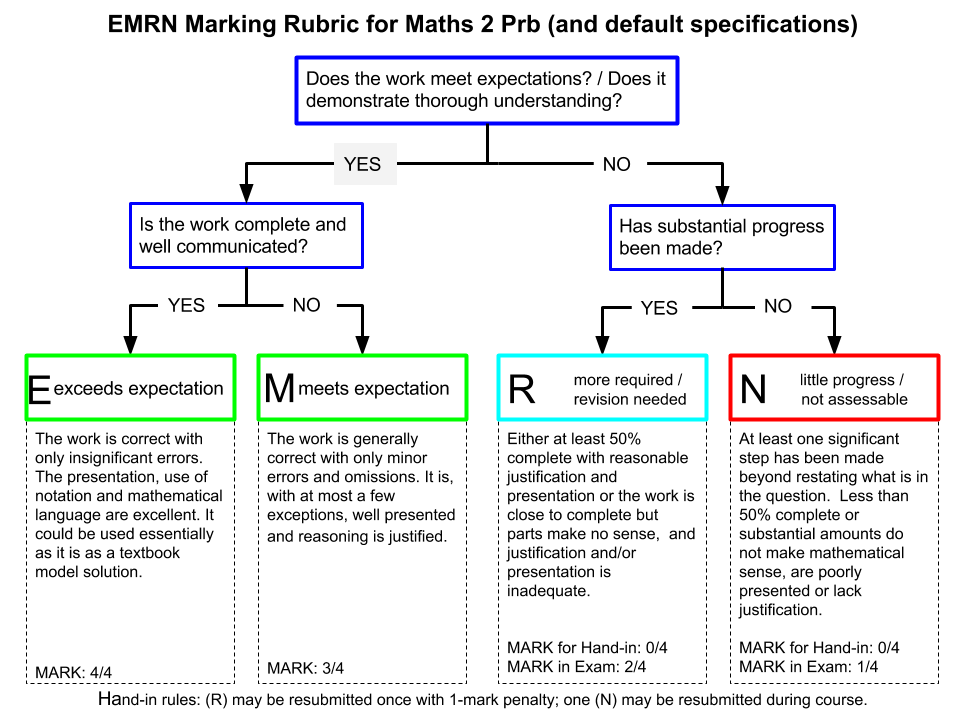
\includegraphics[width=21cm,angle=270]{images/EMRN_Rubric.png}
\end{table}

\section{Problems}

\ssp 
Your friend rolls two D6 and keeps them hidden from you. You ask your friend, ``is there at least one six?'' and he replies ``yes''.  What is the probability that he has rolled a double? 
\end{e} 

\sss
The probability is $1/11$. This is because there are exactly 11 equally likely possible rolls containing at least one six, but only one of them is a double. 
\end{s}

Yah-Tze Same problem and rules, but now the aim is throw five D6 until all are showing the same?  (Challenge --- be careful of an ``edge case''!)


\ssn{Definitions and notation}
An \emph{event} in probability is something that either does or does not happen. The mathematical way this is expressed is that we identify an event with the subspace of the sample space where it happens. 

So, for example, if we toss a coin 3 times a possible event is that we obtain precisely one H.  This event is identified with the subspace 
 \[
 A=\{ TTH, THT, HTT \} \subseteq \{ TTT, TTH, THT, THH, HTT, HTH, HHT, HHH \}. 
 \]
 
If we have another event $B$ defined to be ``the first coin is a T'' then we can consider the event that both $A$ and $B$ happen. This event is denoted $A \cap B$ since it corresponds to the intersection of the two sets. In this case, 
 \[
     A \cap B = \{ TTH, THT \} . 
 \]
\end{n}

\ssn{Definition}
Let $A$ and $B$ be events. We say that $A$ and $B$ are \emph{independent} if  
\[
     \PP( A \cap B ) = \PP(A) \PP(B). 
 \]
\end{n}

\ssn{Examples}
\begin{enumerate}
\item Roll two D6 and let $A$ be the event that the first roll is a `6' and $B$ be the event that the second roll is a `6'.  Then ``$A\cap B$'' is the event of rolling double 6.    We know $\PP(A) = \PP(B) = 1/6$ and also that $\PP(\text{double 6}) = 1/36$.  So $A$ and $B$ are independent.
\item Consider the example of tossing 3 coins as just above. We have $\PP(A) = 3/8$ since it corresponds to 3 of the 8 equally likely outcomes. Also $B = 1/2$.   As we observed, $A \cap B$ corresponds to two outcomes and so $\PP(A \cap B) = 1/4$. We see that $A$ and $B$ are not independent. 
Intuitively, this is because \emph{knowing the first coin is a T changes the probability of there being one H overall (from $3/8$ to $1/2$); one even is affecting the outcome of the other.}
\end{enumerate}
\end{n}

Generalise this formula to the case where $X$ has a Binomial distribution with parameters $n,p$ and $k=np$ is an integer.  Find an approximate formula for $\PP(X=k)$ when $b=n$ is large.  



\ssn{Sample spaces and events}
As we have seen, a \emph{sample space} $S$ is the set of all possible outcomes of an experiment or process. We identify some subsets of $S$ as being \emph{events}, which will be the things that have probabilities associated with them. We require the collection of vents to have the following properties. 
\begin{enumerate}[S1]
\item The whole sample space $S$ and the empty set $\emptyset$ are events. 
\item If $A \subseteq S$ is an event then $A^c = S \setminus A$ is also an event. (It is the event that happens precisely when $A$ does not happen.)
\item Secondly, if $A_1,A_2, \dots$ is a finite or countable collection of events then $\bigcup_i A_i$ is an event. It corresponds to at least one of the $A_i$ happening. 
\end{enumerate}
Events are going to be the occurrences to which we can associate probabilities.  In all the examples we have considered previously, every subset of $S$ is an event. But we will see later that for continuous distributions this is not the case. 
\end{n}

Take three D6 and roll them until you have a triple (i.e.\ all faces show the same number) when you stop. The rules are as follows. On the first round, roll all three. On the second round, you can keep any number of the dice and roll the rest. (So if you have two showing the same, you keep those and roll the third.) Continue for as many rounds as it takes to get the triple.  What are the probabilities of succeeding on (a) the first round; (b) the second round and (c) the third round?  (Give exact answers, and also evaluate these as a decimal.)

\ssn{Sampling with and without replacement}
I roll a D6 twice. What is the probability that I get a `1' followed by a `6'? Answer: $(1/6) \times (1/6) = 1/36$. 

I have a pack of 10 cards numbered 1 to 10. I choose one at random and then \emph{without replacing it} choose another from the pack.  (a) What is the probability that the first card is the `1'?  (b) What is the probability that the second card is the `10'.   (c) What is the probability that I get the `1' followed by the `10'? 

The answers to (a) and to (b) are both $1/10$.  To calculate the answer to (c) consider taking the first card: clearly the probability of its being `1' is $1/10$. Now however there are only 9 cards left and so \emph{knowing that the first card was a `1'} the probability of getting a `10' with the second draw is $1/9$. Therfore the answer (draw a tree if you need to) is $(1/10) \times (1/9) = 1/90$.   

Drawing a `1' first time has made it a little more likely that we draw a `10' next. \emph{The two events are not independent.} 

In terms of conditional probabilities we are reasoning as follows. 
\[
 \PP(\text{`1' then `10'}) = \PP(\text{first is `1'})   
 \, \PP( \text{second is `10'} \st \text{first is `1'}). 
\]

Finally, in more abstract language, let $A$ be the even that the first draw is the `1' and let $B$ denote the event that the second draw is the `10'. Then 
 \[
 \PP( A \cap B ) = \PP(A)\, \PP(A \st B) = \frac{1}{10} \, \frac19 = \frac1{90}. 
 \]
\end{n}

As a first example, suppose we roll two D6.  What is the probability that there is at least one `6' showing?   To solve this, let $A_1$ be the event that the first die shows a `6' and let $A_2$ be the event that the second die shows a `6'.  Clearly $\PP(A_1) = \PP(A_2) = 1/6$. The event $A_1 \cap A_2$ is rolling `double-6' and so $\PP(A_1 \cap A_2) = 1/36$. The event we are interested in is $A_1 \cup A_2$ and by the formula 
 \[
    \PP(A_1 \cup A_2) = \frac16 + \frac16 - \frac1{36} = \frac{11}{36}. 
 \]
 We computed this also by a simple table or tree previously. 
 
 
 \ssn{Definition} 
Let $A,B$ be events with $\PP(B) \not=0$. Then the \emph{conditional probability of $A$ given $B$} is defined by 
 \[
    \PP(A \st B) = \frac{ \PP( A \cap B)}{\PP(B)}. 
 \]
\end{n}

\ssn{Comments}
The conditional probability $\PP (A \st B)$ is the probability of $A$ occurring if we already know that $B$ has occurred.  

We have used conditional probabilities before, particularly in tree calculations.  Generally we were using the alternative form 
\[
    \PP(A\cap B) = \PP(A \st B) \PP(B) . 
\]
\end{n}

\begin{figure}
\begin{minipage}{0.47\textwidth}
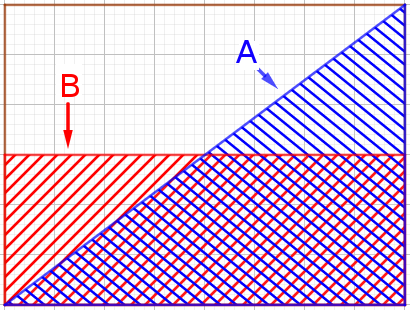
\includegraphics[width=0.95\textwidth]{images/conprob2.png} 
\end{minipage}%
\begin{minipage}{0.47\textwidth}
Imagining probabilities as being proportional to area, $\PP(A)=\PP(B) = 1/2$ and $\PP(A \cap B)=3/8$ (see picture on left). Thus $\PP(A \st B) = 3/4$. 

\hspace*{2ex}
If we ``zoom in on $B$'' as below we see that $A$ occupies three quarters of $B$. 

\vspace*{2ex}
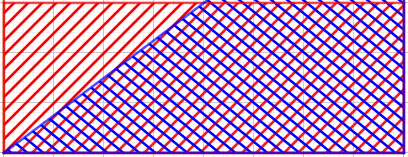
\includegraphics[width=0.95\textwidth]{images/conprob2r.png}
\end{minipage}
\caption{Conditional probabilities, imagining probability proportional to area}
\end{figure}

\ssn{Proposition}
\begin{itemize}
\item If $\PP(B) \not=0$ then $A,B$ are independent if and only if $\PP(A \st B) = \PP(A)$.
\item If $\PP(A) \not=0$ then $A,B$ are independent if and only if $\PP(B \st A) = \PP(B)$.  
(The proof is immediate from the definition.) 
\end{itemize}
\end{n}

\ssp 
We will solve a problem that caused some consternation recently on twitter. We know that the expected number of rolls of a D6 until we get a `6' is $6$. The question asked was this: what is the expected number of rolls until we get a `6', conditioned on the whole sequence consisting of even numbers? 
\begin{enumerate}
\item What do you imagine the answer might be, if you had to guess?
\item Describe how you would do an experiment to try and answer the question numerically. 
\item I give you a D6 and ask you to do some experiments to find this expected value.  What should you do? 
\item Take as sample space $S$ the set of all sequences of rolls of a D6, terminating with the first occurrence of a `6'.  What is the probability of a particular sequence of length $k$?  How many such sequences are there?  (This should fit with the formula for a geometric distribution.) 
\item You roll a D6 until you get a `6'. What is the probability that you have rolled no odd numbers in the process.  (You will need to 
\end{enumerate}

\end{e}



\ssn{Another tree example} 
An ``$n$-sided die'' is a real or imaginary object that chooses an element of $\{ 1,2,\dots, n \}$ uniformly randomly.  We will call such a thing a ``D$n$''. You can buy a D$n$ for many values of $n$ in gaming shops. 

Player A rolls a D3 and player B rolls a D4 and the winner is the person who rolls the higher number. In this rather unfair game, what are the probabilities that player A wins, draws and loses?   We will draw a tree, imagining that A rolls first. We will write $a$ for A's roll. Note how the labels on the arrows emerging from a node add up to $1$.  

\tikzset{
  treenode/.style = {shape=rectangle, rounded corners,
                     draw, align=center,
                     top color=white, bottom color=blue!20},
  root/.style     = {treenode, font=\Large, bottom color=red!30},
  env/.style      = {treenode},
  branch/.style = {treenode, bottom color=blue!10},  
  dummy/.style    = {circle,draw}
}
\tikzstyle{level 1}=[level distance=3.0cm, sibling distance=4.5cm]
\tikzstyle{level 2}=[level distance=8.5cm, sibling distance=1.5cm]
\begin{tikzpicture}
  [
    grow                    = right,
    edge from parent/.style = {draw, -latex},
    every node/.style       = {font=\normalsize}
  ]
\node[root]{Start}
child {
    node[branch]{$a=1$}
    child {
        node[env]{A win $(p=\frac{0}{12})$}
        edge from parent node[above,pos=0.7] {$0$}
        }
        child {
        node[env]{draw~~$(p=\frac{1}{12})$}
        edge from parent 
        node[above,pos=0.7] {$\frac{1}{4}$}
        }
       child {
        node[env]{B win $(p=\frac{3}{12})$}
        edge from parent 
        node[above,pos=0.7] {$\frac{3}{4}$}
        }  
    edge from parent 
    node[above] {$\frac{1}{3}$}
    }
    child {
    node[branch]{$a=2$}
    child {
        node[env]{A win  $(p=\frac{1}{12})$}
        edge from parent 
        node[above,pos=0.7] {$\frac{1}{4}$}
        }
        child {
        node[env]{draw~~$(p=\frac{1}{12})$}
        edge from parent 
        node[above,pos=0.7] {$\frac{1}{4}$}
        }    
        child {
        node[env]{B win $(p=\frac{2}{12})$}
        edge from parent 
        node[above,pos=0.7] {$\frac{2}{4}$}
        }    
    edge from parent 
    node[above] {$\frac{1}{3}$}
    }
    child {
    node[branch]{$a=3$}
    child {
        node[env]{A win $(p=\frac{2}{12})$}
        edge from parent 
        node[above,pos=0.7] {$\frac{2}{4}$}
        }
        child {
        node[env]{draw~~$(p=\frac{1}{12})$}
        edge from parent 
        node[above,pos=0.7] {$\frac{1}{4}$}
        }   
        child {
        node[env]{B win $(p=\frac{1}{12})$}
        edge from parent 
        node[above,pos=0.7] {$\frac{1}{4}$}
        }   
    edge from parent 
    node[above] {$\frac{1}{3}$}
    };           
\end{tikzpicture}


You should check all the calculations. As an example, near the top there is an edge labelled ``$2/4$'' that leads to a win for A.  What that means is that \emph{if we know that A has rolled a 3}, then the probability that A wins is $2/4 = 1/2$. This is true because when $a=3$, A wins if B rolls a 1 or 2 but draws or loses if B rolls 3 or 4. 
\end{n}



\ssn{A diversion (optional)}
I have a floor ruled with parallel lines unit distance apart. I take some stiff, thin wire of length $L$ and bend it into a reasonably smooth curve of some sort that will lie flat on the plane.  I toss the wire in the air so that it lands randomly on the floor.  What is the expected number of times the curved wire meets the ruled lines? 

You could approximate the the wire by a large number $n$ of straight line segments of length $L/n$. Let $X_j$ be the random variable that is $1$ if the $j$-th segment crosses a line and zero otherwise. Then 
 \[
    X = X_1 + X_2 + \dots + X_n 
 \]
 where $X$ is the total number of times the curve meets the lines. 
 
 Then the expected number of crossings of the whole curve in this approximation is given by 
 \[
 \EE(X) =  \EE\left(  \sum_{j=1}^n X_j \right) =  \sum_{j=1}^n \EE(X_j).
  \]
Now, $\EE(X_j)$ must be independent of $j$: it is the expected number of crossings of the lines on the floor by a randomly tossed line segment of length $L/n$.  The conclusion of all this is that the expected number of crossings must be proportional to $L$.  

Now a circular piece of wire of length $\pi$ has diameter $1$ and however it lands, it must meet the lines twice. So that fixes the constant of proportionality:
\[
      \EE(X) = \frac2\pi L 
\]

An interesting special case is to consider a straight line segment of unit length. In that case (neglecting a probability zero possibility of its (just) meeting two lines), $X$ takes only the values $0$ and $1$. Because of that, $\EE(X) = \PP(X=1)$. So the conclusion is that if you drop a unit length line segment randomly onto parallel lines unit distance apart, there is a probability of $2/\pi$ that it will cross a line. 
\end{n}

\end{document} 
